\documentclass[a4paper]{article}

\usepackage{graphicx}
\usepackage[english]{babel}
\usepackage[utf8x]{inputenc}
\usepackage[T1]{fontenc}
\usepackage{sectsty}
\usepackage{pdfpages}
\usepackage[section]{placeins}
\usepackage{float}% If comment this, figure moves to Page 2
\usepackage{listings}
\usepackage{caption}
\usepackage{subcaption}
\usepackage{parskip}

\setlength\parindent{0pt}
%\setlength{\parskip}{\baselineskip}

%\sectionfont{\fontsize{12}{15}\selectfont}

\begin{document}

\title{Software Architecture Process And Management}
\date{}
\author{Computer Science 4th Year, Created By Monkeys}
\maketitle
\newpage

\tableofcontents
\newpage


\section{Introduction}

PRINT MODIFIABILITY GPES CASE STUDY STUFF!\\
WIKIPEDIA AGILE, V-MODEL, SPIRAL, DEVOPS\\
ADD TACTICS!!

\subsection{Learning Outcomes of the course}
\begin{itemize}
\item Integrate knowledge of software architecture to capture \textbf{quality attribute} requirements for a system, \textbf{evaluate proposed architectures} and create options for \textbf{improvement}.

\item Analyse and justify complex \textbf{trade-off decisions} between \textbf{competing software architectures}.

\item Evaluate the \textbf{strengths} and \textbf{weaknesses} of software architecture in support of particular approaches to \textbf{design}, \textbf{process} and \textbf{management} for a particular system and make \textbf{recommendations} on the \textbf{choice of process} for that system.

\item Working in a group to \textbf{critically reflect} on aspects of the \textbf{software architecture literature} and practice to create a resource that support their learning in software architecture.
\end{itemize}

\subsection{What is Success for a Large Project?}
A large project will be considered successful if:
\begin{itemize}
\item The software is delivered on schedule
\item Development costs are within budget
\item The software meets the needs of users
\end{itemize}

\subsection{Software Architecture}

\underline{\textbf{Software Architecture Definitions}}
\begin{enumerate}
\item The software architecture of a system is the \textbf{set of structures} needed to reason about the system, which comprise software elements, relations among them and properties of both. (Bass, Clements, Kazman 2013)
\item A software system's architecture is the set of \textbf{principal design decisions} about the system (R.N Talyor et al)\\
\end{enumerate}

\underline{\textbf{Architecture is a collection of structures}}\\
We observe three frequently types of structure:
\begin{enumerate}
\item \textbf{Modular Structure}: static structure that focuses on how the functionality is divided up, structured, and assigned to development and implementation teams.
\item \textbf{Component and Connector structure}: runtime structures that focus on how components interact.
\item \textbf{Allocation structures}: mapping to organizational, development, installation, execution environments.\\
\end{enumerate}

\underline{\textbf{Architecture is an Abstraction}}\\

Architecture is used to \textbf{suppress} detail that is unimportant for the reasoning we are doing. In particular it \textbf{abstracts away} from the private details of \textbf{implementation details} of specific methods.\\

** All systems have architectures (even if people have forgotten them) **\\

Complicated systems are embedded in organisation and we can often see architecture through practice:
\begin{itemize}
\item \textit{How is the system developed?} -> This will often provide \textbf{clues to structures}.
\item \textit{How is the maintenance, evolution, issue reporting dealt with?} -> This will often help with \textbf{modularity}.
\item \textit{What are the failure characteristics of the system in operation?} -> This will often suggest \textbf{component and connector structure}.
\end{itemize}


\subsection{Case Study: General Practice Extraction System}

"The General Practice Extraction Service (GPES)" is an IT system designed to allow NHS organizations to extract data from \textbf{all} GP practice computers. \textit{This is because different GP's have different contracts and therefore use different software to save patient data.}\\

Basic idea is to create an API to query every system from all different software's created for different GP's. This will allow generic extraction of \textbf{patient data} regardless of their GP.

% IMAGE: GPES Customers
\begin{figure}[H]
\centering
\begin{subfigure}{1\textwidth}
  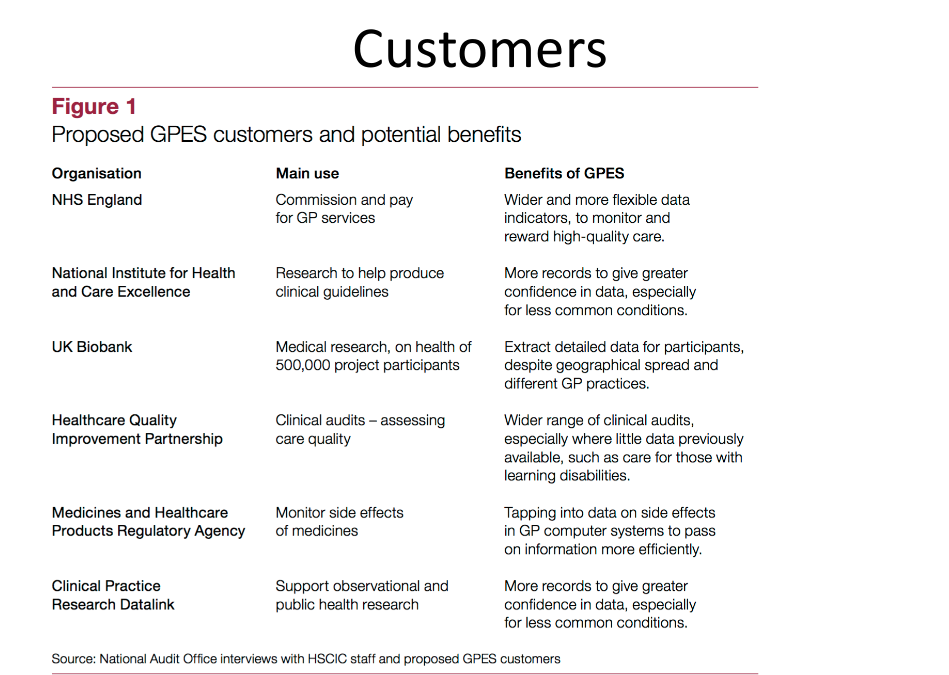
\includegraphics[width=1\linewidth]
  {images/1-customers.png}
\end{subfigure}
%\caption{-}
\end{figure}


% IMAGE: GPES Structure
\begin{figure}[H]
\centering
\begin{subfigure}{1\textwidth}
  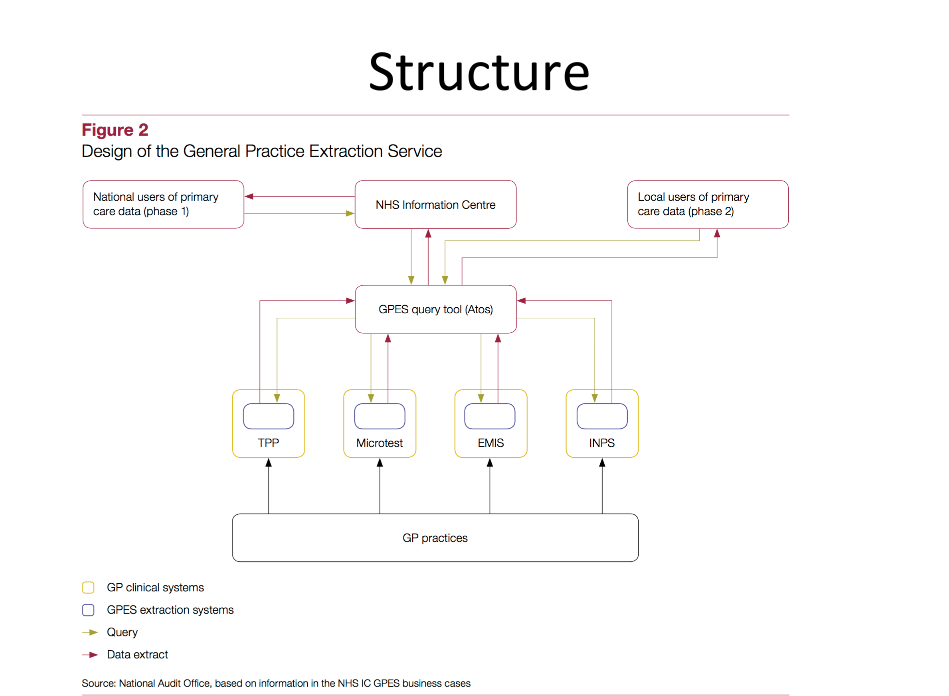
\includegraphics[width=1\linewidth]
  {images/1-structure.png}
\end{subfigure}
%\caption{-}
\end{figure}

% IMAGE: GPES Timeline
\begin{figure}[H]
\centering
\begin{subfigure}{1\textwidth}
  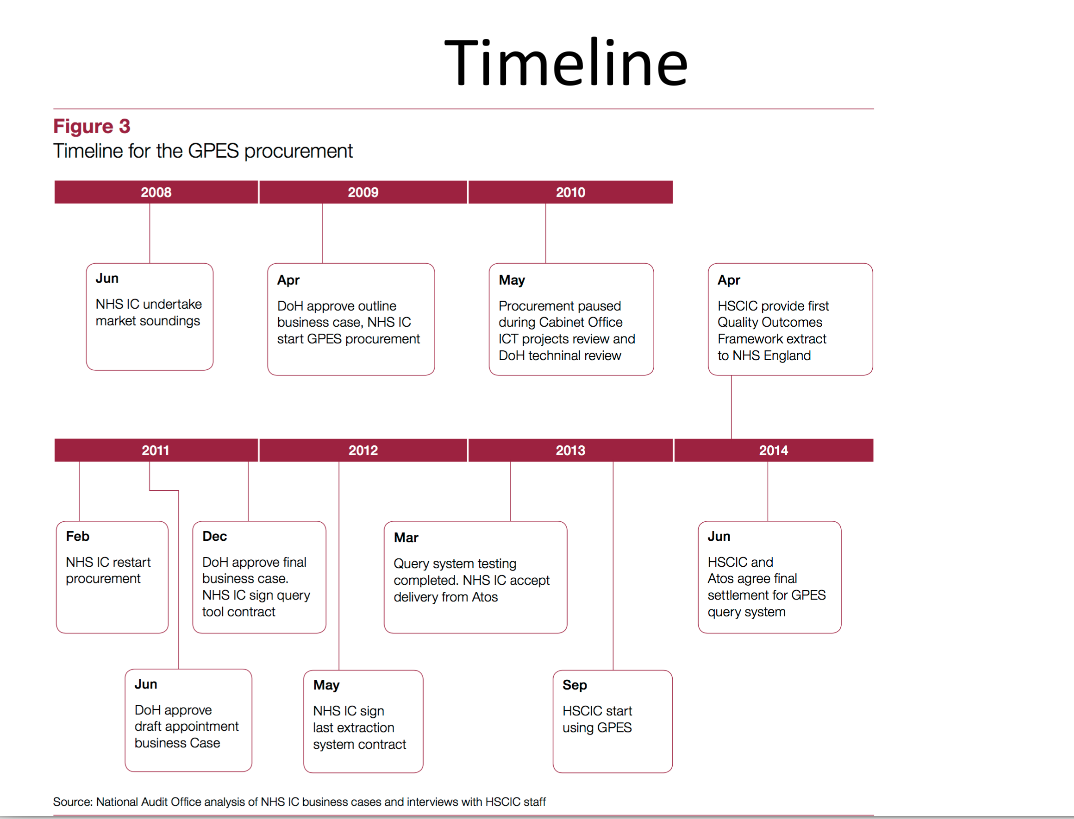
\includegraphics[width=1\linewidth]
  {images/1-timeline.png}
\end{subfigure}
%\caption{-}
\end{figure}


\underline{\textbf{National Audit office Conclusion of the GPES Project}}
\begin{itemize}
\item The project has been significantly delayed and many customers have yet to receive data.
\item Mistakes in the original procurement and contract management contributed to the losses of public funds. This occurred through asset write-off's and settlements with suppliers
\item Only \textbf{one} customer, \textit{NHS England} has so far received data from GPES.\\
\end{itemize}

Originally the business plan for GPES said the service would start in \textbf{2009-2010}. It actually took until \textbf{2014} for the first extraction to take place. The total expected loss for the GPES project rose from \textbf{£14 million} to \textbf{£40 million} during the \textit{planning} and \textit{procurement stage}.\\

\underline{\textbf{Data Extract Issues}}
\begin{itemize}
\item First GP system suppliers were asked to fulfil a common query language for the extraction process (this was not in their interest as it would cost them alot to makes these changes to their current systems and thus pretty much refused to do so).
\item This requirement then changed to each GP system supplier creating their own logical 'business rules' which would be used to extract the data. (Different for each supplier, one API to query each supplier to extract data)
\item NHS IC's using a non-competitive procurement approach, in-addition to the changes in design both contributed to the restrictive process for \textit{extracts}.
\item HSCIC (the successor of the NHS IC) has continued to use the GPSOC framework to require data sharing between NHS systems. \textit{The new framework (2014) states that the principal clinical system suppliers must provide an interface method for third-party system uses.}

\item \textbf{HSCIC cannot do wide range nor scale of data extracts. Due to the design of the GPES system and the restrictions in the supplier contracts. (Over 100 different extracts have been requested) HSCIC estimate that they will only be able to design 24 new extracts in 2015-16}\\
\end{itemize}

% IMAGE: GPES Issues
\begin{figure}[H]
\centering
\begin{subfigure}{1\textwidth}
  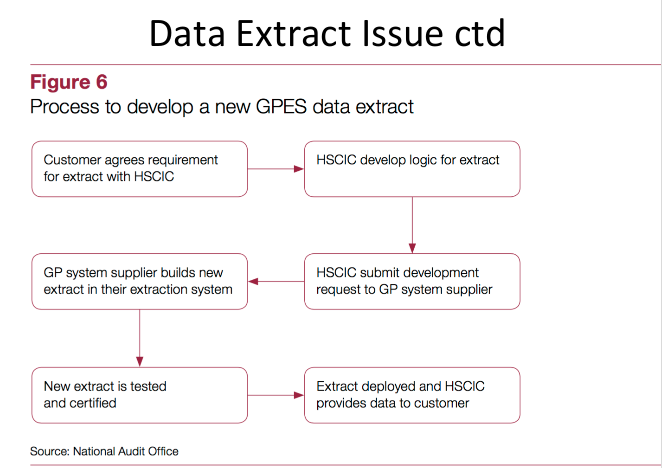
\includegraphics[width=1\linewidth]
  {images/1-issues.png}
\end{subfigure}
%\caption{-}
\end{figure}

% IMAGE: GPES Issues Concluded
\begin{figure}[H]
\centering
\begin{subfigure}{1\textwidth}
  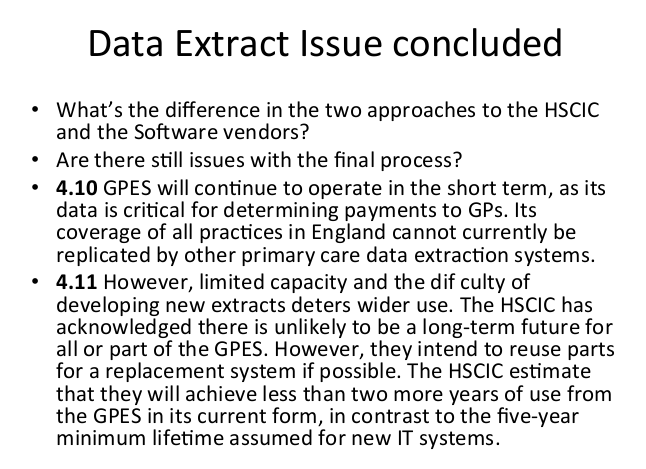
\includegraphics[width=1\linewidth]
  {images/1-issues-concluded.png}
\end{subfigure}
%\caption{-}
\end{figure}
\newpage

\section{Basic Concepts of Architectures}
\subsection{What is good architecture?}
The architecture is appropriate for the \textbf{context of use}. E.g. 3-tier e-commerce architecture is not appropriate for a avionics project.\\

Guidance on 'good architecture' focuses on:
\begin{itemize}
\item \textbf{Process}
\item \textbf{Structure}\\
\end{itemize}



Software architecture should capture the \textbf{principal design} decisions about the system. The \textbf{Blueprint} for software architecture focuses on:
\begin{itemize}
\item Structure
\item Component behaviour
\item Component interaction and how that influences \textbf{Quality Attributes} of the \textit{systems}.\\
\end{itemize}

\subsection{Process}
Architect teams are often small and \textbf{maintains the integrity} of the architecture. The architecture is \textit{justified} in relation to a \textbf{prioritized list of quality attributes} that need to be managed. \textbf{Stakeholders interests} are documented and are used to build the type of architecture that will reflect them.\\

Architecture is often evaluated in terms of \textit{how well it delivers the quality attributes}. Software architectures are often chosen to allow \textbf{incremental implementation}. (I.e Low coupling, high cohesion)

- Definitions for coupling and cohesion!

\subsection{Structure}

The structure of architecture will differ depending on the requirements of the software, often the following are utilised:
\begin{itemize}
\item \textbf{Modularity} $\rightarrow$ Hides information, separates concerns, allows good robust interfaces that are unlikely to change
\item Well known \textbf{patterns and tactics} are often implemented
\item Architecture built to NOT depend on \textbf{particular versions of tools}, or \textbf{special features} \textit{unless its essential!}
\item Modules \textit{producing} data should be \textbf{separate} from those \textit{consuming} data
\item Usually a complex mapping between \textbf{modules} \textit{(static structure)} and \textbf{components} \textit{(dynamic structure)}
\item MINIMISE the number of ways of \textbf{interaction between components}
\item The architecture should clearly \textbf{identify resource contention issues} and deal with them. (E.g. network capacity, minimise network throughput using different techniques [EXC])\\
\end{itemize}

\underline{\textbf{Prescriptive vs Descriptive Structures}}\\
\textbf{Prescriptive} structure is what we use to model the system before it is built. It is the aim the architect has while generating the blueprint \textit{(UMLAsBlueprint, forward engineering)}, however it is often to \textit{tidy} and unrealistic to be able to model the architecture of a system.\\

\textbf{Descriptive} structure is usually made after the system has been created. It is used to describe the entire system, how the \textbf{components} interact, the responsibilities of each \textbf{module} \textit{(usually extremely messy)} etc ...

\subsection{The Importance of Architecture}
Software Architecture has several uses:
\begin{enumerate}
\item Enables us to manage the \textbf{key attributes} of a system
\item Allows reasoning about and managing \textbf{change}
\item Allows predictions of \textbf{key quality attributes}
\item Allows \textbf{improved communication} between stakeholders
\item Defines \textbf{constraints} on the software's implementation
\item Provides the basis for \textbf{evolutionary prototyping}
\item Is the key artefact for reasoning about \textbf{cost} and \textbf{scheduling}
\item Focuses on the assembly of \textbf{components} rather than the \textbf{creation/implementation} of components\\
\end{enumerate}

Other uses are:
\begin{itemize}
\item \textit{Reflects the structure of an organisation}
\item \textit{Can be used as the transferable, reusable model at the heard of a product line}
\item \textit{Restricts design alternative and channels developer effort in a coordinated way}
\item \textit{Provides the basis for training new team members}
\end{itemize}

\subsection{Managing Attributes and Change}
It is a fact that the majority of software projects will undergo requirements change. This may also change \textbf{key quality attributes} of the system. The idea is to use architecture that will minimise the change to the \textit{architecture} and allow the system to be \textbf{modifiable} utilising the same abstract \textbf{architectural} ideas.\\

Managing change can be reasoned about on three levels:
\begin{enumerate}
\item Inside an element \textit{[cheapest]}
\item Between elements maintaining the architecture \textit{[can be costly]}
\item Requiring architecture change (we wish to avoid this as much as possible) \textit{[most expensive change]}
\end{enumerate}

\subsection{Prediction of Attributes}
We can attempt to predict the \textbf{key quality attributes} of the system based on \textit{requirements} and possible (logical) \textit{system extensions} in the future. Planning for these changes will minimise need for architectural change, which in turn will \textbf{reduce the cost} in future work.\\

\textbf{** Models should be able to be built based on the predictions of the attributes and requirements **}


\subsection{Communication Between Stakeholders}
A well documented architecture allows \textbf{improved communication} between stakeholders. Some examples of how the documented architecture can help with communication are the following:
\begin{itemize}
\item User has particular requirements in terms of user experience
\item Customer needs to know about schedule, budget and meeting regulations in their market
\item Project manager needs to know the dependences in terms of the modules and components
\end{itemize}
\underline{\textit{These might be accommodated by different views of the system that are consistent}}

\subsection{Early Design and Constraints}
Early design carries the \textit{most fundamental} design decisions, e.g:
\begin{itemize}
\item What the \textbf{key quality attributes} are
\item The \textbf{architecture form/type} that will give the best control over these attributes
\item The characterisation of the behaviour of the architecture elements\\
\end{itemize}

% IMAGE: Constraints
\begin{figure}[H]
\hskip-1.5cm\begin{subfigure}{1.1\textwidth}
  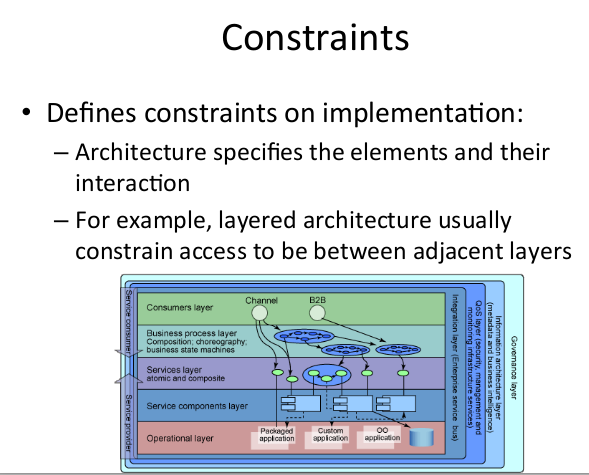
\includegraphics[width=1.2\linewidth]
  {images/2-constraints.png}
\end{subfigure}
%\caption{-}
\end{figure}

\subsection{Evolutionary Prototyping}
\textbf{Evolutionary Prototyping} allows a system to be constantly tested under real conditions as it is being developed. As \textit{bugs} are detected they are fixed and tested in the next prototype. Examples of systems that used \textbf{evolutionary prototyping} are:
\begin{itemize}
\item Plug and Play - early experience of the BASE functionality + extensibility.
\item Real time architectures - early experience with scheduling. \textit{(Worse case execution times guide design and deployment)}
\end{itemize}

\subsection{Cost and Scheduling}
Reasoning about the \textbf{following topics} allows for effect cost and scheduling in a software project:
\begin{itemize}
\item Capturing dependencies
\item Estimation of required efforts for different sections
\item Allocating effort to elements
\item Understanding of how elements influence each other
\item Use architecture to interpret bottom-up estimates from teams working on elements
\end{itemize}

\subsection{Product Line (Model)}
The \textbf{product line} model is a \textit{transferable and reusable} model. \textbf{Elements} are assets that compose to give new \textit{functionality}. The architecture provides the means to \textbf{compose the elements}. A planned approach allows the reuse of architectural elements \textit{(think object inheritance)}.

\subsection{Component Level \& Channelling Development}
At the component level we focus on the \textbf{assembly} of components rather than the \textbf{creation} of them! With well designed elements and architecture we can combine elements from different \textbf{producers} \textit{(provided they conform to a standardized interface)}. This provides the following \textbf{benefits}:
\begin{itemize}
\item Decrease time to market
\item More reliability
\item Lower cost
\item Flexibility \textit{(e.g. using multiple or alternate suppliers for a component)}\\
\end{itemize}

\textbf{Channelling Development} restricts alternatives and channels developer effort in a coordinate way. This provides a defined \textbf{context} for the developer. Well defined \textbf{interfaces} and clear ideas of the \textbf{functionality \& quality attributes} are required!\\

\textbf{** The overall goal is to provide clarity on what is an architectural decision and what is a development decision. **}
\newpage


\section{Context Design}
Software architects and architecture have arisen as systems have grown in: \textit{scale}, \textit{economic importance} and \textit{criticality}. Architecture plays different roles in different contexts. The \textbf{main contexts} are:
\begin{itemize}
\item Technical Context
\item Project Life-cycle Context
\item Business Context
\item Professional Context
\end{itemize}
\subsection{Technical Context}
The \textbf{technical context} is whereby the architecture supports technical activity. For example this could be in \textbf{measuring} a statistic, the \textbf{verification \& validation} process, \textbf{compliance} ...\\

The architecture provides a means for controlling \textbf{quality attributes} of the system. In the \textbf{context of design} activities we try and choose architectures that \textbf{enable the attributes} we care most about. We may find through analysing already \textit{existing systems} that specific architectures inhibit (prevent) particular quality attributes.\\

** Architecture does not often have much to say about the functionality of a system, because they provide containers for functionality. **

\subsubsection{Controlling Quality Attributes}

Usually we care about multiple quality attributes at once. Selecting a type of architecture will allow specific quality attributes to be ensured for when it is deployed to the end user. Examples of \textbf{quality attributes} we might care about for a particular system are:

\begin{table}[H]
\begin{tabular}{|l|p{10cm}|}
\hline
QA & Description\\
\hline
Safety & The safety of a system is whereby we worry about ensuring that the \textbf{system only behaves as is intended} and has no additional behaviour that is unspecified.\\
\hline
Testability & The testability of a system ensures that \textbf{elements are clearly isolated}. That we know the \textbf{expected behaviour of components}. We know the \textbf{relations of modules} to track down faulty code and finally we know how the \textbf{components are intended to integrate together} to give overall behaviour.\\
\hline
Availability & The availability of a system is whereby we worry about ensuring there is a \textbf{system to take over}, in the case the original system fails. \\
\hline
\end{tabular}
\end{table}

Other examples of quality attributes include \textbf{performance}, \textbf{usability}, \textbf{interoperability} ...\\

These examples of quality attributes related to the \textbf{actuator monitoring} system that was described in lectures. As actuators are physical devices they will suffer from \textit{'wear and tear'} and eventually break. In safety critical system (for example cars, aeroplanes) these actuators require monitoring in order to prevent worst-case scenario's when they do break, and have them repaired beforehand.\\

The architecture for the actuator monitoring system will be required to hold at least those three quality attributes:
\begin{enumerate}
\item Availability - To ensure it is always monitoring the actuators
\item Safety - To ensure the monitoring system does not deviate from intended behaviour (no false positives or false negative)
\item Testability - To provide certainty that of the safety and availability is should provide.
\end{enumerate}

% IMAGE: Actuator Monitoring Architecture
\begin{figure}[H]
\centering
\begin{subfigure}{1\textwidth}
  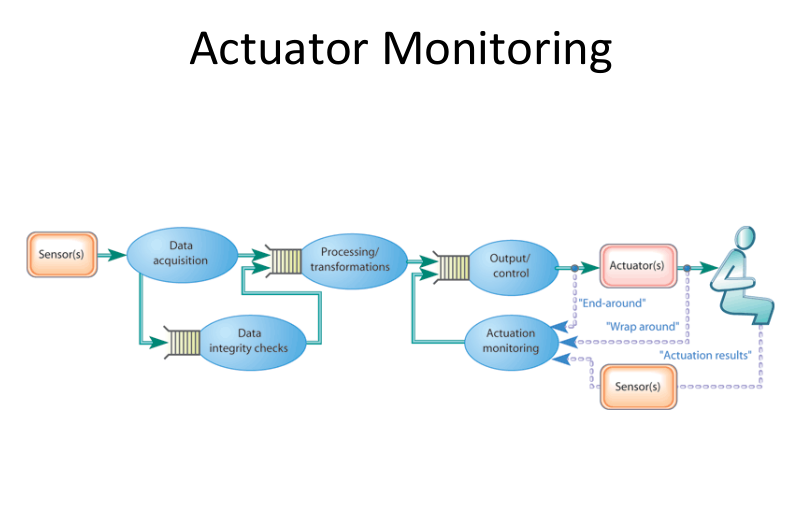
\includegraphics[width=1\linewidth]
  {images/3-actuator-monitoring-architecture.png}
\end{subfigure}
%\caption{-}
\end{figure}


\subsection{Project Life-cycle Context}
The \textbf{project life cycle context} describe how the project will develop over time. The architecture is then created to adopt the life-cycle that is best for a particular project. When creating a project life-cycle the following must be complete \textit{(these are all done best by talking about the architecture)}:
\begin{itemize}
\item Making a business case for the system
\item Understanding the requirements that concern quality attributes
\item Deciding on architecture
\item Documenting architecture
\item Analysing and evaluating architecture
\item Implementing and testing the system based on architecture
\item Ensuring the implementation conforms to the architecture
\end{itemize}

\subsubsection{V-Model}
The \textbf{V-Model} is a development of \textit{waterfall} and explicitly includes architectural design as a stage. It highly focuses on \textbf{requirements based testing} all the way down to the unit level!

% IMAGE: V-Model
\begin{figure}[H]
\hskip-2.5cm\begin{subfigure}{1.2\textwidth}
  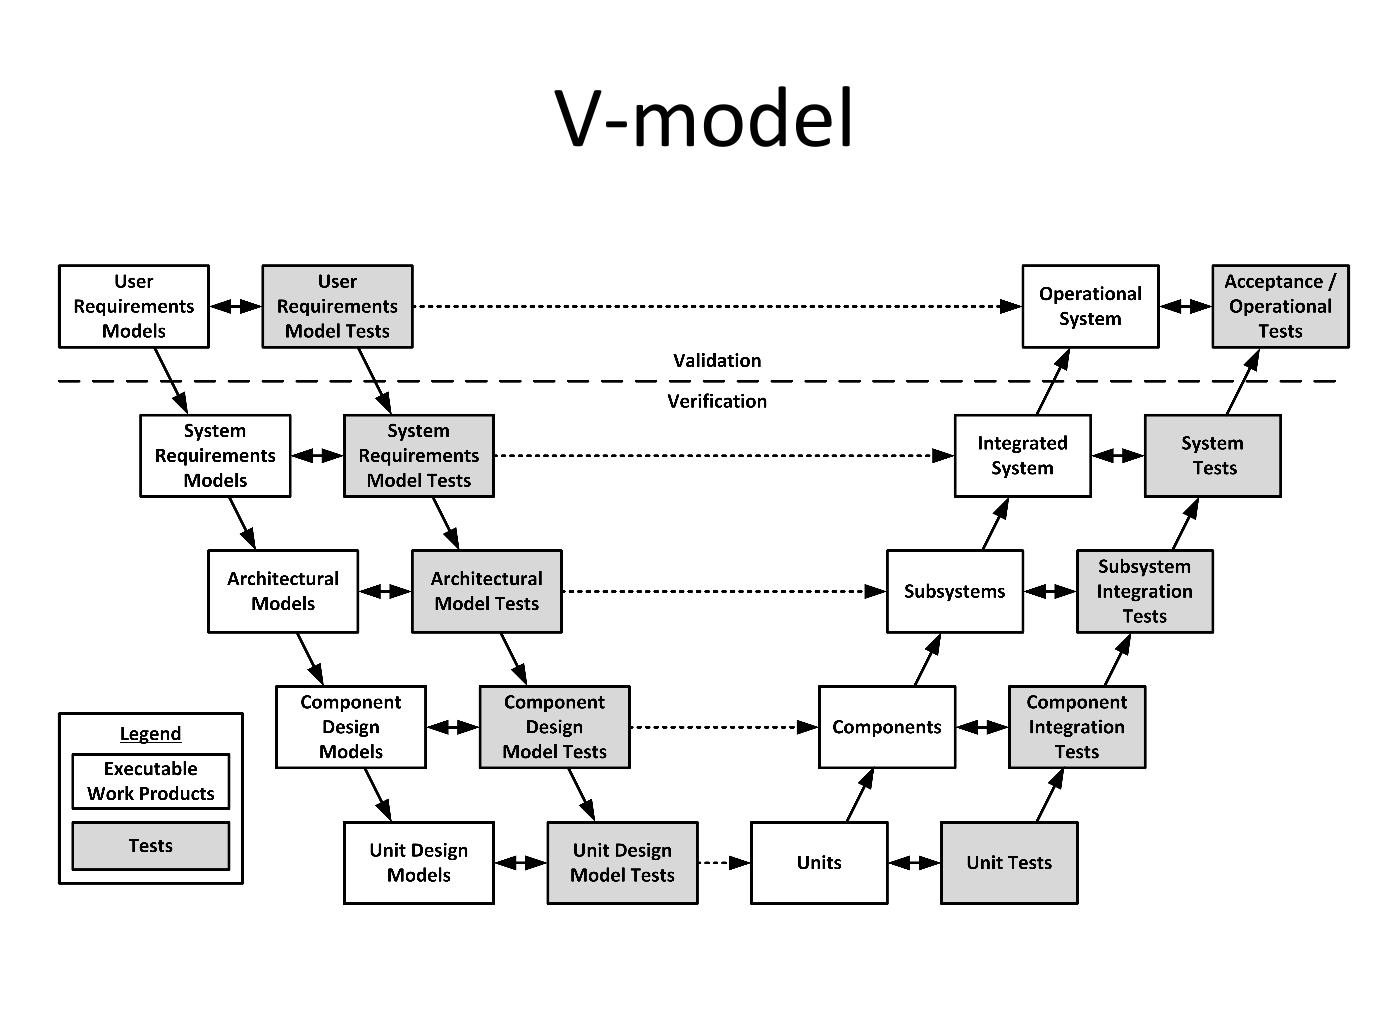
\includegraphics[width=1.2\linewidth]
  {images/3-v-model.png}
\end{subfigure}
%\caption{-}
\end{figure}

\subsubsection{Spiral Model}
The \textbf{(Boehm's spiral model} is a type of \textit{iterative model}. It focuses on project risk management by constantly creating prototypes to be tested all the way through the development life-cycle.

% IMAGE: Spiral
\begin{figure}[H]
\hskip-2.5cm\begin{subfigure}{1.2\textwidth}
  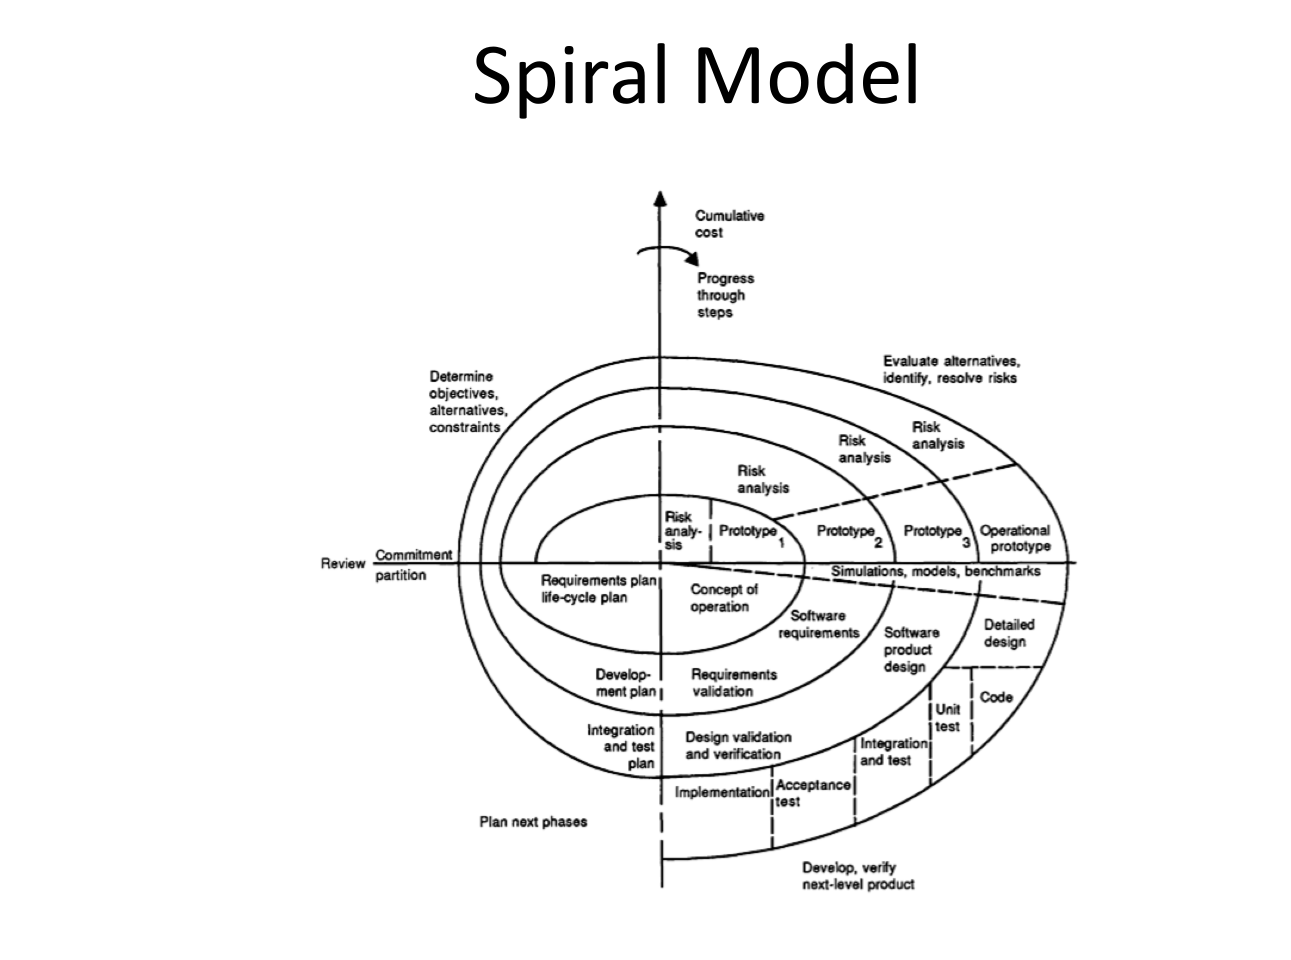
\includegraphics[width=1.2\linewidth]
  {images/3-spiral.png}
\end{subfigure}
%\caption{-}
\end{figure}
\subsubsection{Agile Development}
The \textbf{Agile} development life-cycle is an iterative and incremental method of managing the design and building of a software product. The image below show two different forms of \textbf{agile} development. One with and one without Devops.
% IMAGE: Agile
\begin{figure}[H]
\hskip-2.5cm\begin{subfigure}{1.2\textwidth}
  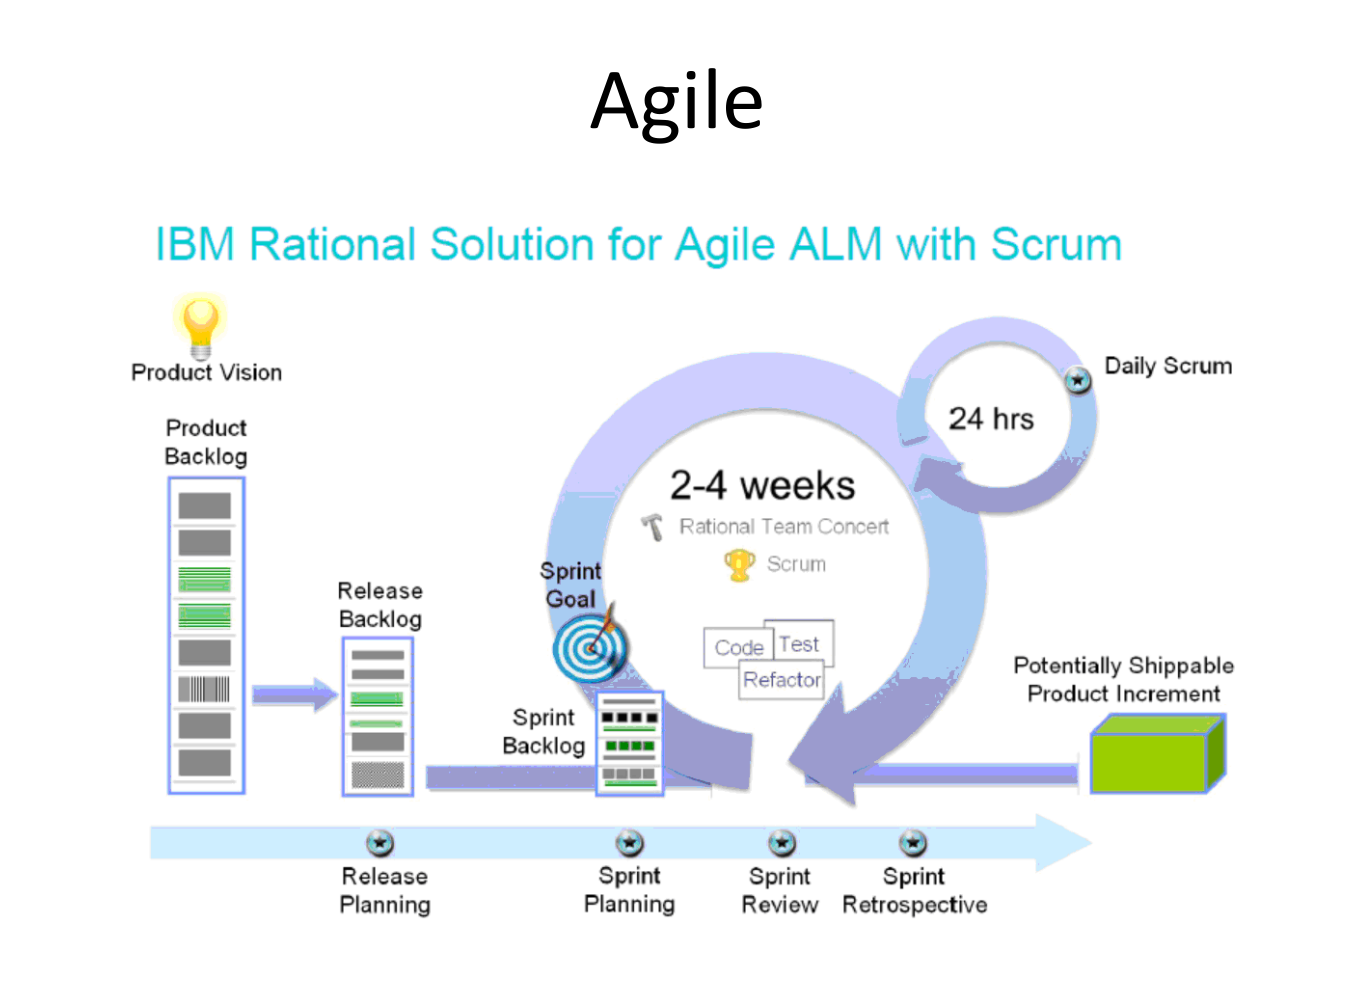
\includegraphics[width=1.2\linewidth]
  {images/3-Agile.png}
\end{subfigure}
%\caption{-}
\end{figure}
\subsubsection{Agile + Devops}
% IMAGE: Agile + Devops
\begin{figure}[H]
\hskip-2.5cm\begin{subfigure}{1.2\textwidth}
  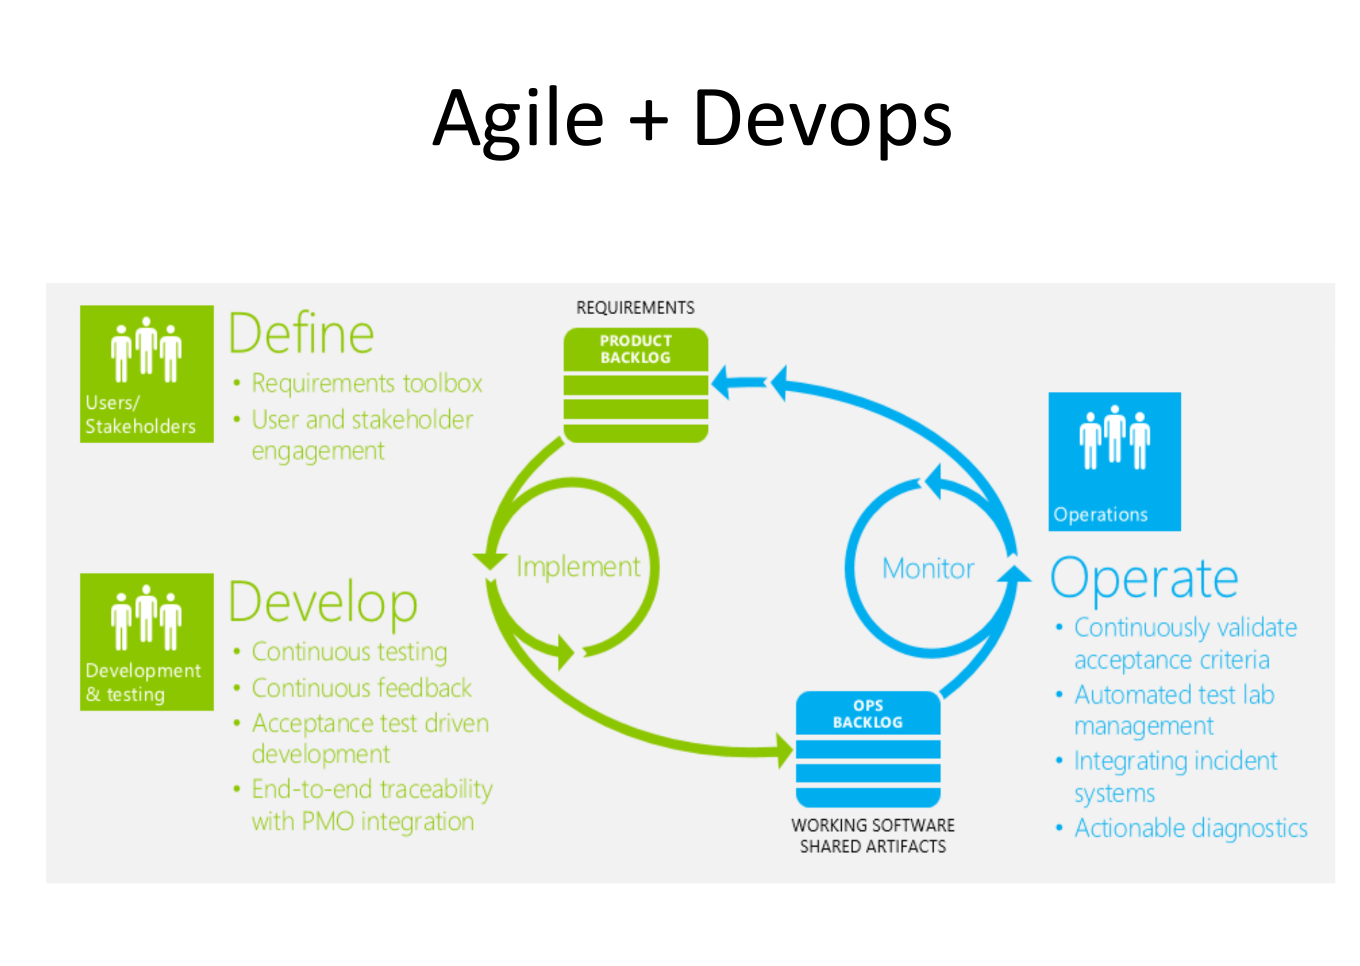
\includegraphics[width=1.2\linewidth]
  {images/3-ADevops.png}
\end{subfigure}
%\caption{-}
\end{figure}
\subsection{Business Context}
The \textbf{business context} is discussed in later lectures. Two aspects we cover are:
\begin{enumerate}
\item How the organisation structure of stakeholders can drive architectural decisions and shapes decisions taking around architecture.
\item How architectural expertise drives the structure of development organisation in terms of their functional units and interrelationships.
\end{enumerate}
\subsection{Professional Context}
The architectural perspective gives you as a professional:
\begin{itemize}
\item A way of describing your expertise
\item Your skills as an architect will be recognised within organisations you work within
\item You can use architecture as a way of describing your past experience
\item You can specialise in particular classes of architecture (e.g. financial architecture)
\end{itemize}
\subsection{Domain-Specific Software Architecture}

\underline{\textbf{Design in the Technical Context}}\\
Design is a mixture of \textbf{creativity} and the use of \textbf{knowledge} that is institutionalised in the context. This takes the form of \textbf{reusable structures}. These reusable structures also influence other aspects of context, helping to shape \textbf{processes, organisations} and \textbf{professions}. We can plot different sorts of \textbf{architectural structures} depending on the degree to which it is \textbf{specific to a domain} and the extent to which it \textbf{influences the system}.\\

% IMAGE:
\begin{figure}[H]
\hskip-2.5cm\begin{subfigure}{1\textwidth}
  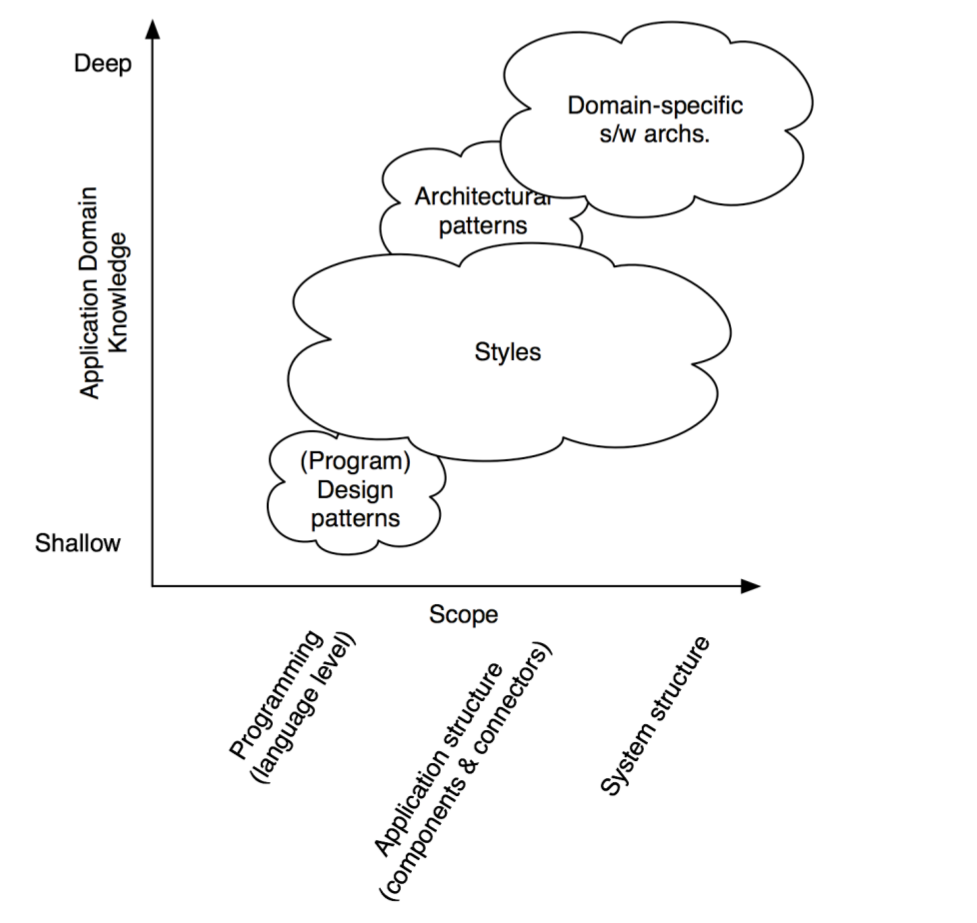
\includegraphics[width=1\linewidth]
  {images/3-graph.png}
\end{subfigure}
%\caption{-}
\end{figure}

\underline{\textbf{Domain Specific Software Architectures}}\\
\textbf{DSSA} is a collection of (pre-decided) \textbf{design decisions}. They capture important aspects of a particular task \textbf{(domain)} They are \textbf{common} across a range of systems in the domain and typically will have some predefined structures depending on the attributes we want to control.\\

These are \textbf{not} general purpose because they incorporate many specific characteristics of the \textbf{domain}. The main benefit is the extent to which \textbf{design knowledge is captured}. There are however problems, over time basic information can be forgotten.\\

** Bridge example given, where key information was forgotten regarding the architecture of suspension bridges (from the 19th century). This results in a bridge collapsing because of wind. **
\subsection{Architectural Patterns}

An architectural pattern is a set of \textbf{architectural design decisions} that are applicable to a \textbf{recurring design problem}, and \textbf{parametrized} to action for different \textbf{software development contexts} in which that problem appears.\\

They are similar to \textbf{DSSA} but capture less of the behaviour and attributes of the system. They are \textbf{more general} because they are intended to abstract a common \textbf{pattern over several domains}.

Three common architectural patterns that are used are listed below:
\begin{enumerate}
\item State Logic Display: Three-Tiered Pattern
\item Model View Controller Pattern
\item Sense Compute Control Pattern\\
\end{enumerate}

\textbf{Contexts shape design.} The \textbf{technical context} identifies features we want to control and \textbf{packages} a range of other properties. Standard architectures (\textit{patterns and domain specific architectures DSSA}) \textbf{package these}. The other context we consider also help to shape the choice of architecture.\\

\textbf{** In design we use pre-decided strcutures and then alter/extend them as and when we need too. **}


% IMAGE:
\begin{figure}[H]
\hskip-2.5cm\begin{subfigure}{1.2\textwidth}
  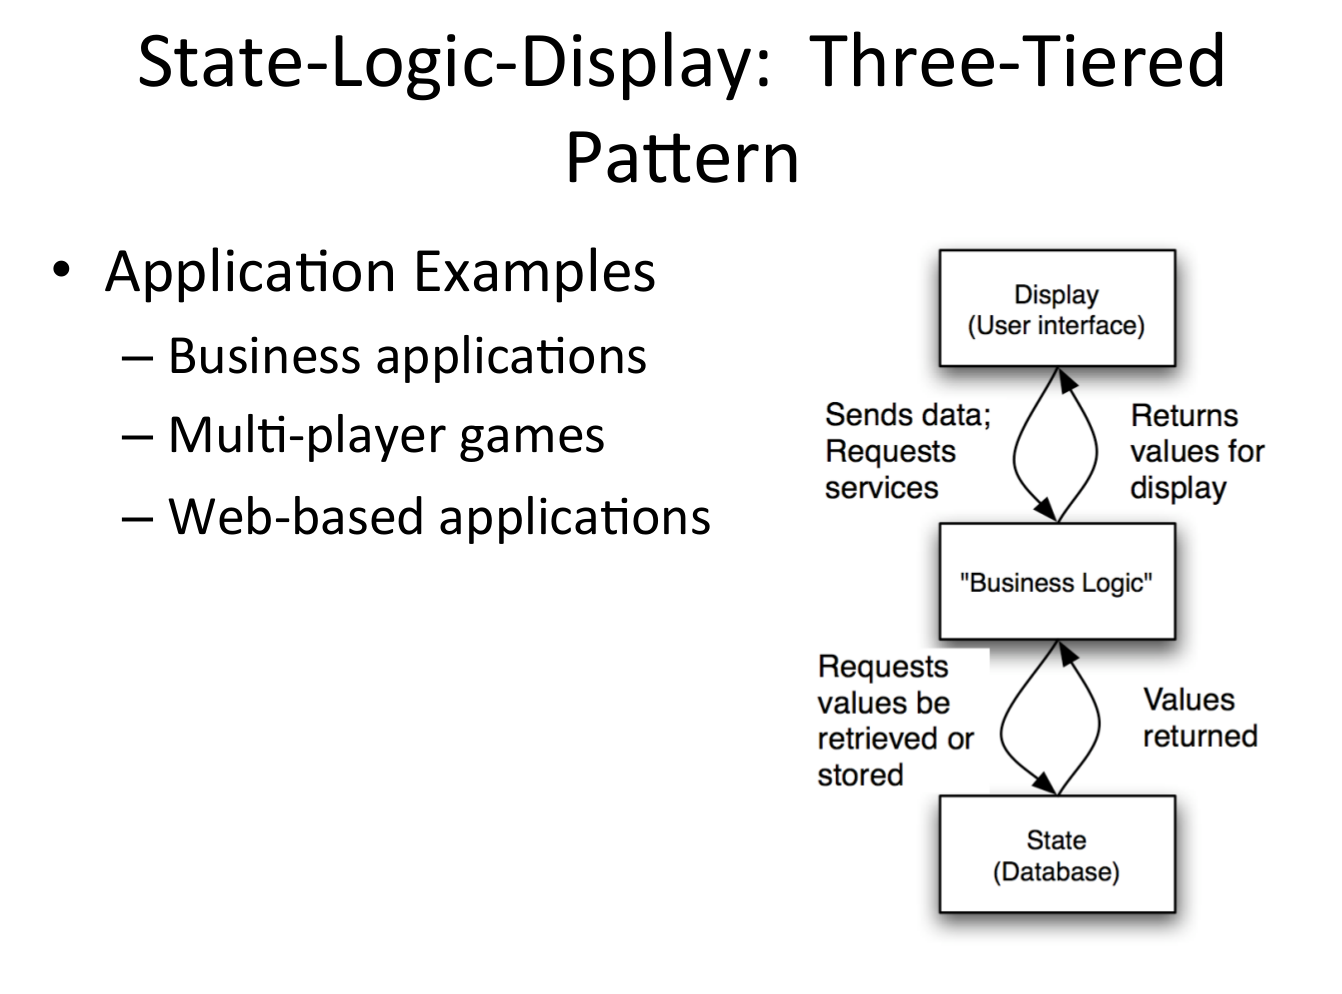
\includegraphics[width=1.2\linewidth]
  {images/3-SLD-pattern}
\end{subfigure}
%\caption{-}
\end{figure}

% IMAGE:
\begin{figure}[H]
\hskip-2.5cm\begin{subfigure}{1.2\textwidth}
  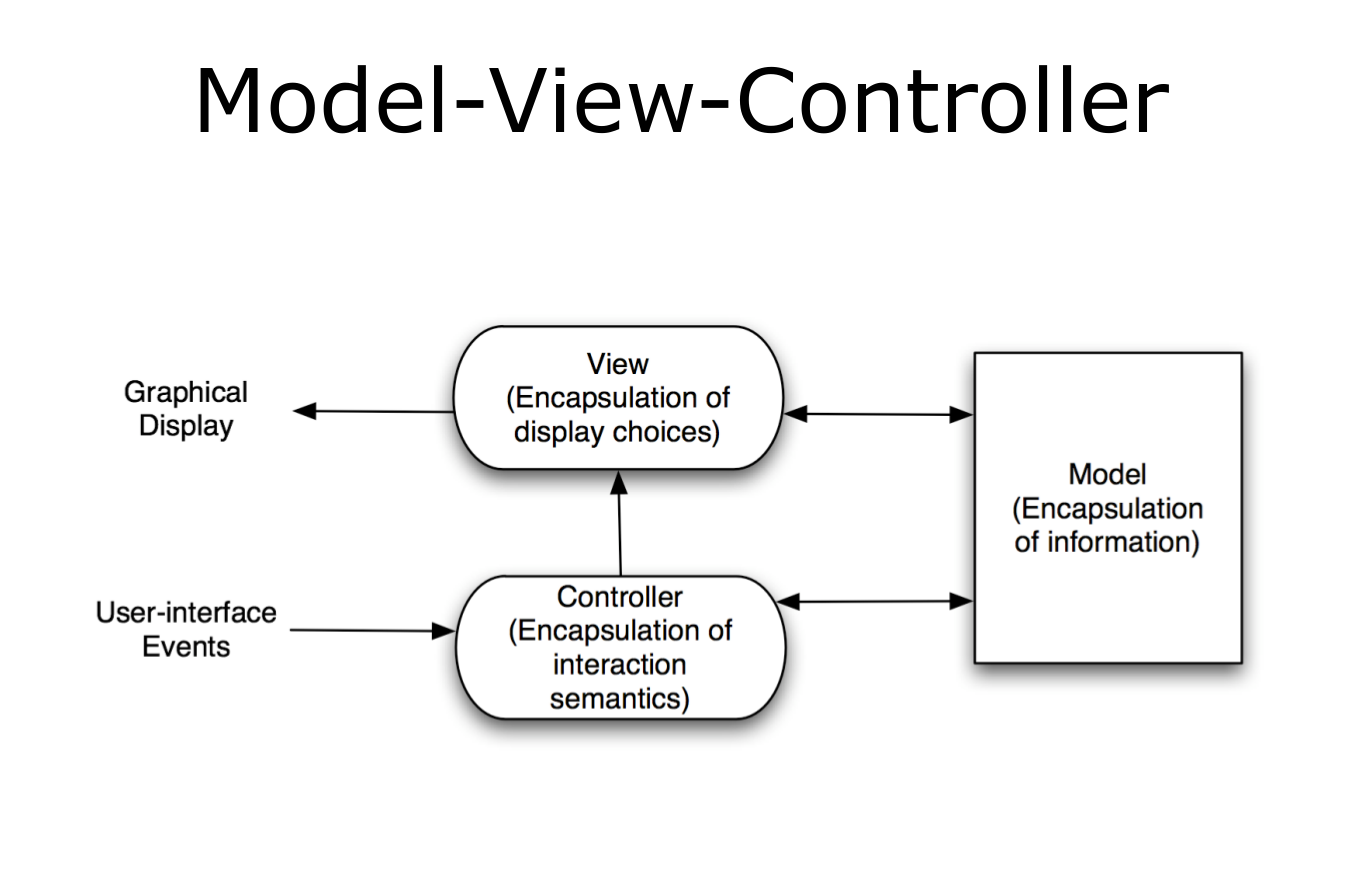
\includegraphics[width=1.2\linewidth]
  {images/3-model-view-controller.png}
\end{subfigure}
%\caption{-}
\end{figure}


% IMAGE:
\begin{figure}[H]
\hskip-2.5cm\begin{subfigure}{1.2\textwidth}
  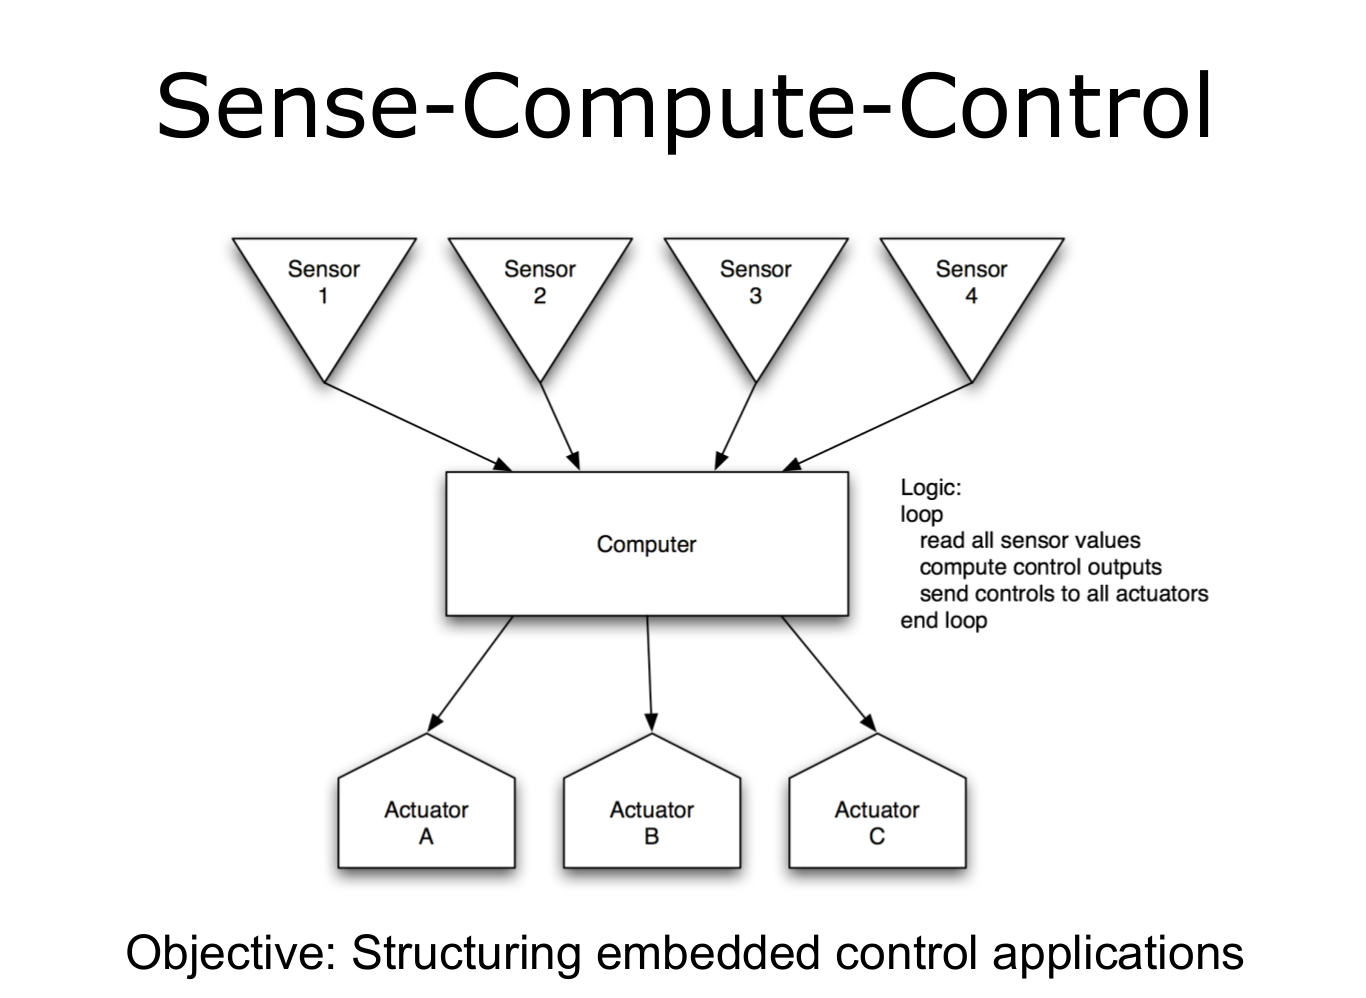
\includegraphics[width=1.2\linewidth]
  {images/3-sense-compute-control.png}
\end{subfigure}
%\caption{-}
\end{figure}
\newpage

\section{Quality Attributes}

Quality Attributes specify, usually quantitatively, the \textbf{requirements} on particular parts of \textbf{functionality} or on the \textbf{whole system}. Software Quality Attributes are the \textbf{benchmarks that describe systems intended behaviour} within the environment for which it was built. The quality attributes provide the means for measuring the fitness and suitability of a product.

\textbf{** Quality Attributes are non-functional requirements **}

\subsection{Stakeholders}
\textbf{Stakeholders represent} different (typically conflicting) \textbf{perspectives on the system} and attempt to influence the architect. The \textbf{architect needs to trade-off the different influences and resolve the conflict.} e.g. - Marketing might want to have a big market but maintenance would prefer system to be simple.

\begin{figure}[h]
\centering 
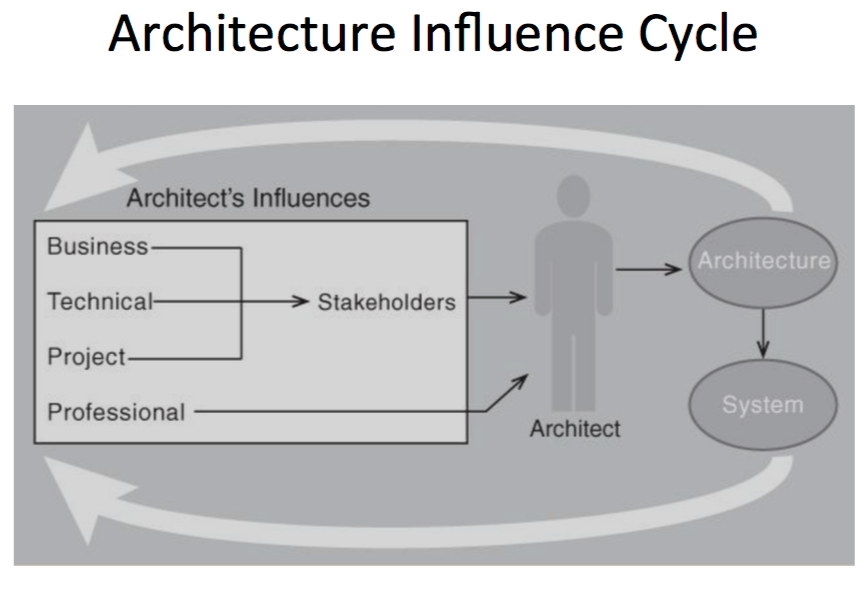
\includegraphics[scale=0.3]{images/influencecycle.png}
\end{figure}

\subsection{Functional Requirements}
These specify what the system does, architecture is important to them as they structure the containers that hold functionality. 

\textbf{** Functional requirements are things the system does. **}

\subsection{Constraints}
These are decisions that have already been taken e.g. we will use the Java programming language (because we have a Java development team available) or the system will only support certain web browsers


\subsection{Problems with Quality Attributes}
\begin{itemize}
\item Often \textbf{quality attributes} are \textbf{not testable}. \textit{(e.g. what does it man to say something is modifiable or usable or dependable or resilient?)}

\item It can be difficult to \textbf{map from a concern about the system} to a quality attribute. \textit{(For example, a high failure rate in some transaction could be a performance issue or it could be an availability issue)}

\item Communities around a \textbf{particular quality attribute have developed their own terminology} \textit{(e.g. security has attacks, performance has events etc)}
\end{itemize}

\textbf{One Solution: } explicitly state the use case of a quality attribute scenario, this aids the avoidance of some issues.

\subsection{Quality Attribute Scenarios}
\textbf{Quality attribute} scenario's have the following components:
\begin{enumerate}
\item \textbf{Source of Stimulus}: Person or another System
\item \textbf{Stimulus}: An action the system responds to. 

\textit{(e.g. using the wrong configuration specification for the system)}
\item \textbf{Environment}: Captures wider aspects of the system
\item \textbf{Artifact}: Part of the system that is stimulated
\item \textbf{Response}: Activity resulting from stimulus
\item \textbf{Response measure}: Measure of the response so that the scenario is testable \textit{(e.g time taken to detect wrong config)}
\end{enumerate}

\begin{figure}[H]
\centering 
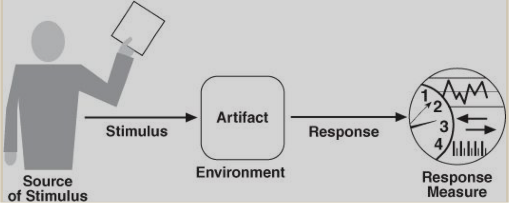
\includegraphics[scale=0.7]{images/QA-general.png}
\end{figure}

Each quality attribute has a \textbf{general scenario} that it \textbf{tries to capture with its components}. This acts like a guide for the architect.

\begin{figure}[H]
\centering 
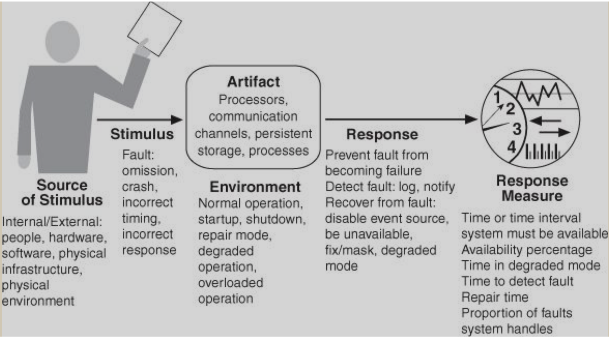
\includegraphics[scale=0.7]{images/availability-general.png}
\end{figure}

\subsection{Architectural Tactics}
\textbf{Architectural tactics} are a way of documenting routes to achieve a particular quality attribute (non-functional) requirement. They are a \textbf{design decision} that influence the achievement of a quality attributes \textbf{response}. \textit{(They are more \textbf{primitive} than design patterns!)}.

Tactics are based on a \textbf{single} quality attribute and do NOT take into account \textbf{trade-off's}. Usually they are more generic and need to be \textbf{specialised} to a specific context. It allows the architect to \textbf{enumerate possible design decisions}.

** If our architecture fails the scenario, because we can't detect the error arising from the fault in one of our tasks, we look at the tactics. **

\subsection{Categories of Architectural Design Decisions}
There are seven broad categories of \textbf{design decisions}:

\begin{enumerate}
\item Allocation of Responsibilities
\item Coordination Model
\item Data Model
\item Management of Resources
\item Mapping Among Architectural Elements
\item Binding Time Decisions
\item Choice of Technology
\end{enumerate}


\subsubsection{Allocation of responsibilities}
\textbf{Identify the most important responsibilities} and determine how to allocate these to runtime and static elements. These are often \textbf{specific} to a quality attribute. 

\textit{For example in the case of availability fault detection is an important responsibility that will be further decomposed and distributed in the architecture.}


\subsubsection{Coordination Model}
Components in the architecture \textbf{interact with one another via a collection of mechanisms}. This is called the coordination model. Things it takes into account are:
\begin{itemize}
\item What \textbf{elements in the system} need to coordinate with one another.
\item What \textbf{properties} \textit{(e.g timing, security)} does the coordination need to have
\item The \textbf{mechanisms and their properties} \textit{(e.g. state fullness, synchrony, delivery guaranties)}
\end{itemize}

\subsubsection{Data Model}

\textit{How data is created and destroyed?}

Data \textbf{access methods, operations} on the data and the \textbf{properties} of the data are all included in the Data Model. 

We also need to decide on how the data would be \textbf{organised, stored, backed up} and \textbf{recovered} in case of data loss. It also includes maintaining \textit{meta-data} that controls the interpretation of the data.


\subsubsection{Management of resources}
We can have both \textbf{hardware} \textit{(e.g. CPU, memory, battery)} and \textbf{software} \textit{(buffers, processes)} resources which need to be managed. Management includes:
\begin{itemize}
\item \textbf{Identification} of the resources need to be managed.
\item The \textbf{system element} should manage a resource.
\item Work out \textbf{sharing strategies} and how to arbitrate (resolve) in \textbf{contention situations}
\item Consider the \textbf{consequences of running out of a resource} (e.g. Memory).
\end{itemize}

\subsubsection{Mapping Among Architectural Elements}
We have 2 types of mapping:
\begin{itemize}
\item \textbf{Mapping between different types of elements in the architecture} 
\textit{e.g. between static development structures and threads or processes}
\item \textbf{Mapping between software elements and environment elements} 
\textit{e.g. from process to specific processors.}\\\\
\end{itemize}


Some important mappings: 
\begin{itemize}
\item Code $\rightarrow$ runtime structures
\item Runtime elements $\rightarrow$ environment
\item Data model elements $\rightarrow$ data stores
\end{itemize}

\subsubsection{Binding Time Decisions}
Binding time decisions \textbf{introduce allowable ranges of variation}. This variation can be bound at \textbf{different times in the software life cycle} by different entities from design time by a developer to runtime by an end user. 

\textit{A binding time decision establishes the scope, the point in the life cycle, and the mechanism for achieving the variation.}

The decisions in the other six categories have an associated binding time decision. \textbf{Examples of such binding time decisions include the following}:

\begin{itemize}
\item For \textbf{allocation of responsibilities}, you can have build-time selection of modules via a parameterized makefile.

\item For \textbf{choice of coordination model}, you can design runtime negotiation of protocols.

\item For \textbf{resource management}, you can design a system to accept new peripheral devices plugged in at runtime, after which the system recognizes them and downloads and installs the right drivers automatically.

\item For \textbf{choice of technology}, you can build an app store for a smartphone that automatically downloads the version of the app appropriate for the phone of the customer buying the app.\\
\end{itemize}


When making \textbf{binding time decisions}, you should consider the \textbf{costs to implement the decision} and the \textbf{costs to make a modification} after you have implemented the decision. 

\textit{For \textbf{example}, if you are considering changing platforms at some time after code time, you can insulate yourself from the effects caused by porting your system to another platform at some cost. Making this decision depends on the costs incurred by having to modify an early binding compared to the costs incurred by implementing the mechanisms involved in the late binding.}

\subsubsection{Choice of technology}

\textbf{Every architecture decision must eventually be realized using a specific technology.} This is completed by completing the following points below:

\underline{** Additional Information **}
\textit{Sometimes the technology selection is made by others, before the intentional architecture design process begins. In this case, the chosen technology becomes a constraint on decisions in each of our seven categories. In other cases, the architect must choose a suitable technology to realize a decision in every one of the categories.}\\\\

\begin{itemize}
\item Deciding which \textbf{technologies are available} to realize the decisions made in the other categories

\item Determining whether the \textbf{available tools to support this technology choice} are adequate for development to proceed.

\textit{(IDEs, simulators, testing tools, etc.)}

\item Determining the extent of \textbf{internal familiarity as well as the degree of external support available} for the technology and deciding whether this is adequate to proceed.

\textit{Such as courses, tutorials, examples, and availability of contractors who can provide expertise in a crunch}

\item Determining the side effects \textbf{(consequences)} of choosing a technology

\textit{Such as a required coordination model or constrained resource management opportunities.}

\item Determining whether a \textbf{new technology is compatible} with the existing technology stack. 

\textit{For example, can the new technology run on top of or alongside the existing technology stack? Can it communicate with the existing technology stack? Can the new technology be monitored and managed?}
\end{itemize}
\newpage
\section{QA: Availability}
Some systems we need to	be there whenever they need to be used.	These are usually called \textbf{high availability systems}.	
\textbf{(Examples)} There can be different reasons for high availability:	
\begin{itemize}
\item{999 telephone system}
\item{Interplanetary spacecraft systems}
\item{Electricity supply grid}
\item{Large Computer System Power Supply}\\\\
\end{itemize}

From Hardware, there are two key \textbf{measures} of availability:
\begin{itemize}
\item{MTBF: Mean Time Between Failures}
\item{MTTR: Mean Time To Repair}\\
\end{itemize}
Availability is the probability of the system working, when you ask it to work.\\

$$\textit{availability = }\frac{MTBF}{MTBF+MTTR}$$\\

To maximise the probability, either make the \textbf{time between failures larger}, or a \textbf{shorter repair time}.
\newline
\subsection{Fault, Error, and Failure}
A \textbf{fault} is something in the system.\\
\textit{(e.g. a broken wire, failed component, wrong bit of code ...)}\\
\textit{(Example) A fault in a sorting routine means that under some circumstances it fails to sort an array.}

The system moves into an \textbf{error} state when the fault is activated.\\
\textit{Under these conditions, the system might be assuming an array is sorted but it isn’t.  In this state there is an error in the system because things are not as they should be.}

\textbf{Failure} is the externally observable deviation from intended operation, this can be caused by an error.\\
\textit{If the system uses binary search to look for things in the array, sometimes an item will be in the array but will not be found – this might cause a visible failure  of the system.}


** Most \textbf{high availability systems} try to tolerate or mask faults by detecting erroneous conditions before they move into failure conditions. **


\subsection{General Scenario}

\begin{itemize}
\item{\textbf{Source}: Internal or external sources important to differentiate because different measures are possible.}
\item{\textbf{Stimulus}: Fault causes errors: omission (no result), crash (repeated omissions), timing (late, early), response (incorrect value).}
\item{\textbf{Artifact}: Specifies what has to be available: process, channel, store, …}
\item{\textbf{Environment}: what the mode of operation is: normal, degraded, startup, shutdown, …}
\item{\textbf{Response}:  how to respond to the stimulus }
\item{\textbf{Response measure}: this will be some measure related to the availability or the “liveness” of the artifact}
\end{itemize}

\subsection{Concrete Scenario}

In \textbf{mission critical systems} there is typically a schedule that activates a sequence of tasks in turn.  These take longer or shorter times to complete and the whole set is carried out cyclically. What happens if there is a bug in a task and it never completes?

\begin{itemize}
\item{Cycles through each of the tasks.}
\item{Passes control to one of the tasks}
\item{Waits for control to pass back.}
\item{If one of the task fails, the architecture fails the scenario.}
\end{itemize}


\subsection{Availability Tactics}
\begin{center}
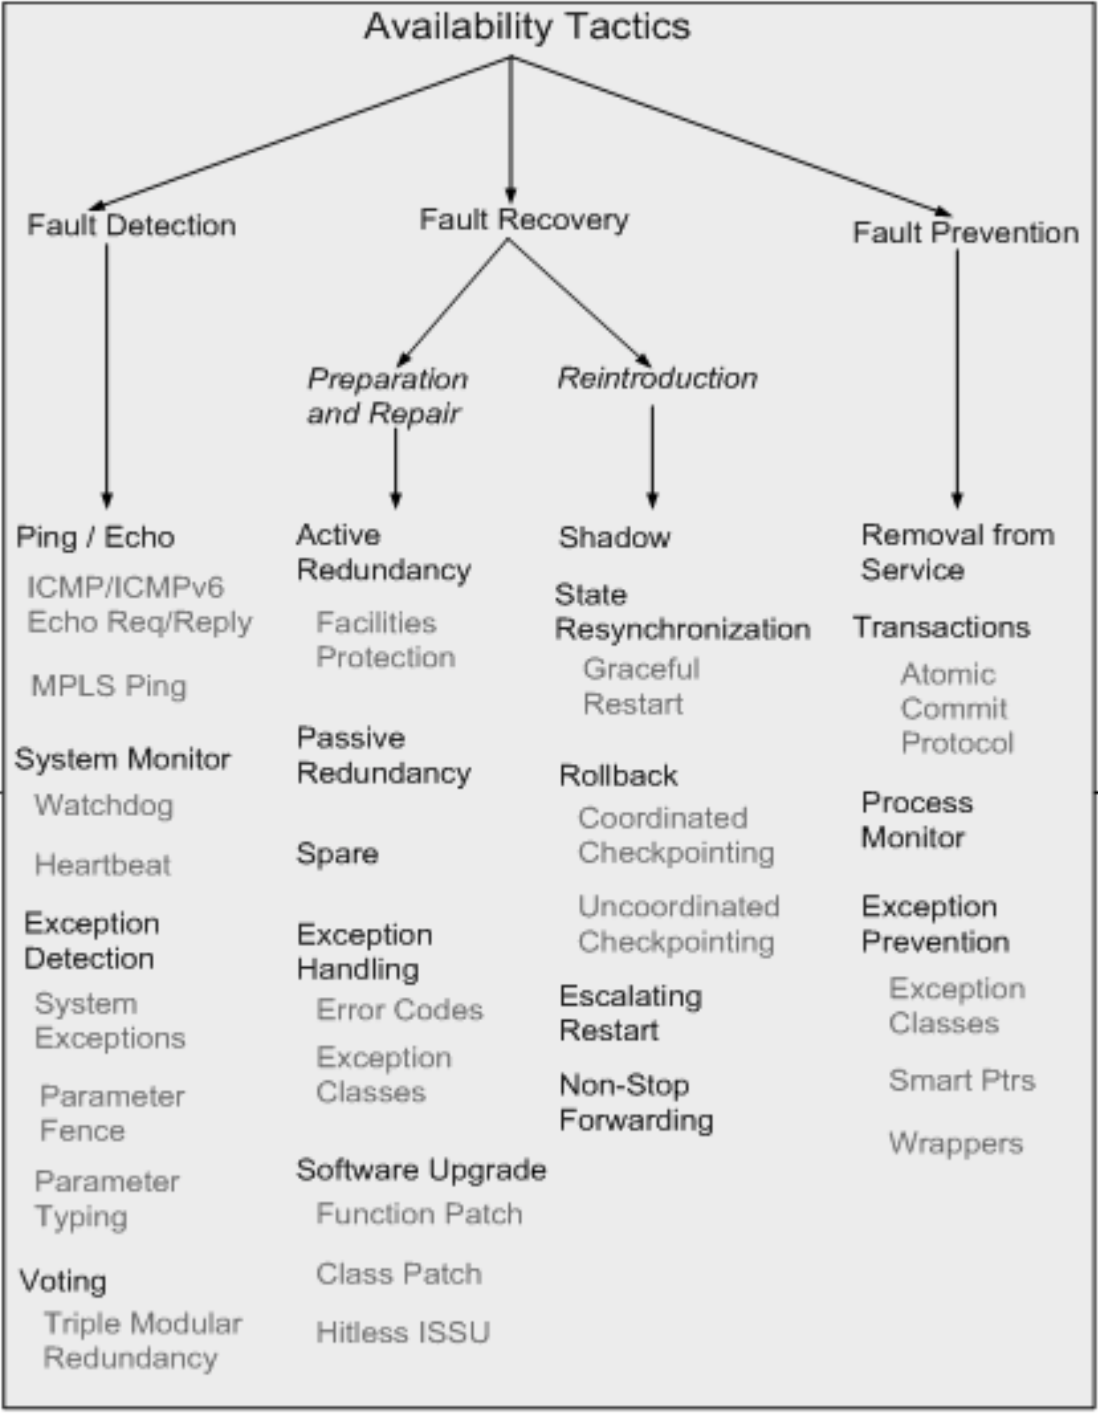
\includegraphics[scale=0.6]{images/abcdefg.png}
\end{center}



\subsubsection{Fault Detection}
\begin{itemize}
  \item
    \textbf{Ping/echo.}
    One component issues a ping and expects to receive back an echo, within a predefined time, from the component under scrutiny. This can be used within a group of components mutually responsible for one task. It can also used be used by clients to ensure that a server object and the communication path to the server are operating within the expected performance bounds. "Ping/echo" fault detectors can be organized in a hierarchy, in which a lowest-level detector pings the software processes with which it shares a processor, and the higher-level fault detectors ping lower-level ones. This uses less communications bandwidth than a remote fault detector that pings all processes.
  \item
    \textbf{Heartbeat (dead man timer).}
    In this case one component emits a heartbeat message periodically and another component listens for it. If the heartbeat fails, the originating component is assumed to have failed and a fault correction component is notified. The heartbeat can also carry data. For example, an automated teller machine can periodically send the log of the last transaction to a server. This message not only acts as a heartbeat but also carries data to be processed.
  \item
    \textbf{Exceptions.}
    One method for recognizing faults is to encounter an exception, which is raised when one of the fault classes we discussed in Chapter 4 is recognized. The exception handler typically executes in the same process that introduced the exception.
\end{itemize}
  
\subsubsection{Fault Recovery}
  \begin{itemize}
  \item
    \textbf{Voting.}
    Processes running on redundant processors each take equivalent input and compute a simple output value that is sent to a voter. If the voter detects deviant behavior from a single processor, it fails it. The voting algorithm can be "majority rules" or "preferred component" or some other algorithm. This method is used to correct faulty operation of algorithms or failure of a processor and is often used in control systems. If all of the processors utilize the same algorithms, the redundancy detects only a processor fault and not an algorithm fault. Thus, if the consequence of a failure is extreme, such as potential loss of life, the redundant components can be diverse.
  \item
    \textbf{Active redundancy (hot restart).}
    All redundant components respond to events in parallel. Consequently, they are all in the same state. The response from only one component is used (usually the first to respond), and the rest are discarded. When a fault occurs, the downtime of systems using this tactic is usually milliseconds since the backup is current and the only time to recover is the switching time. Active redundancy is often used in a client/server configuration, such as database management systems, where quick responses are necessary even when a fault occurs. In a highly available distributed system, the redundancy may be in the communication paths. For example, it may be desirable to use a LAN with a number of parallel paths and place each redundant component in a separate path. In this case, a single bridge or path failure will not make all of the system's components unavailable.
  \item
    \textbf{Passive redundancy (warm restart/dual redundancy/triple redundancy).}
    One component (the primary) responds to events and informs the other components (the standbys) of state updates they must make. When a fault occurs, the system must first ensure that the backup state is sufficiently fresh before resuming services. This approach is also used in control systems, often when the inputs come over communication channels or from sensors and have to be switched from the primary to the backup on failure. Chapter 6, describing an air traffic control example, shows a system using it. In the air traffic control system, the secondary decides when to take over from the primary, but in other systems this decision can be done in other components. This tactic depends on the standby components taking over reliably. Forcing switchovers periodically-for example, once a day or once a week-increases the availability of the system. Some database systems force a switch with storage of every new data item. The new data item is stored in a shadow page and the old page becomes a backup for recovery. In this case, the downtime can usually be limited to seconds.
  \item
    \textbf{Spare.}
    A standby spare computing platform is configured to replace many different failed components. It must be rebooted to the appropriate software configuration and have its state initialized when a failure occurs. Making a checkpoint of the system state to a persistent device periodically and logging all state changes to a persistent device allows for the spare to be set to the appropriate state. This is often used as the standby client workstation, where the user can move when a failure occurs. The downtime for this tactic is usually minutes.
  \item
    \textbf{Shadow operation.}
    A previously failed component may be run in "shadow mode" for a short time to make sure that it mimics the behaviour of the working components before restoring it to service.
  \item
    \textbf{State resynchronization.}
    The passive and active redundancy tactics require the component being restored to have its state upgraded before its return to service. The updating approach will depend on the downtime that can be sustained, the size of the update, and the number of messages required for the update. A single message containing the state is preferable, if possible. Incremental state upgrades, with periods of service between increments, lead to complicated software.
  \item
    \textbf{Checkpoint/roll-back.}
    A checkpoint is a recording of a consistent state created either periodically or in response to specific events. Sometimes a system fails in an unusual manner, with a detectably inconsistent state. In this case, the system should be restored using a previous checkpoint of a consistent state and a log of the transactions that occurred since the snapshot was taken.
\end{itemize}

\subsubsection{Fault Prevention}
\begin{itemize}
  \item
    \textbf{Removal from service.}
    This tactic removes a component of the system from operation to undergo some activities to prevent anticipated failures. One example is rebooting a component to prevent memory leaks from causing a failure. If this removal from service is automatic, an architectural strategy can be designed to support it. If it is manual, the system must be designed to support it.
  \item
    \textbf{Transactions.}
    A transaction is the bundling of several sequential steps such that the entire bundle can be undone at once. Transactions are used to prevent any data from being affected if one step in a process fails and also to prevent collisions among several simultaneous threads accessing the same data.
  \item
    \textbf{Process monitor.}
    Once a fault in a process has been detected, a monitoring process can delete the nonperforming process and create a new instance of it, initialized to some appropriate state as in the spare tactic.
  \end{itemize}


\subsection{WatchDog (Tactic Example)}
A \textbf{watchdog timer} \textit{(sometimes called a computer operating properly or COP timer, or simply a watchdog)} is an electronic timer that is used to detect and \textbf{recover from computer malfunctions}. During normal operation, the computer regularly resets the watchdog timer to prevent it from elapsing, or "timing out". If, due to a hardware fault or program error, the computer fails to reset the watchdog, the timer will elapse and generate a timeout signal. The timeout signal is used to initiate corrective action or actions. The corrective actions typically include placing the computer system in a safe state and restoring normal system operation.\\

\textbf{Use-Cases: } Embedded Systems, Space Probes, or any system where humans cannot easily access the equipment or would be unable to react to faults in a timely manner.

\subsection{Architectural Design Decisions (for availability)}
\begin{itemize}
\item{Allocation of responsibilities}
\item{Coordination model}
\item{Data Model}
\item{Management of resources}
\item{Mapping among architectural elements}
\item{Binding time decisions}
\item{Choice of technology}
\end{itemize}

\subsubsection{Allocation of Responsibilities}

\begin{itemize}
\item{Determine what needs to be high availability (maybe not all functions).}
\item{Responsibility for detecting error (and possible cause).}
\item{Responsibility to log errors}
\item{Responsible respond to a detected error}
\item{Manage sources of events}
\item{Decide on mode of operation}
\item{Decide on how to repair faults}
\item \textbf{In the previous case, assign a watchdog and allocate its responsibility of responding to error}
\end{itemize}

\subsubsection{Coordination Model}
\begin{itemize}
\item{Are the error detection capabilities of the coordination model adequate to detect errors?}
\item{Is the coordination model sufficient to ensure communication and coordination between error detection, log and response.?}
\item{Will coordination work in the presence of error, degraded modes?}
\item{If repair involve replacement of elements will the coordination model allow this?}
\item \textbf{In our example the wakeup between watchdog and controller might be an addition to the coordination mechanism.}
\end{itemize}

\subsubsection{Data Model}
\begin{itemize}
\item{How do error conditions affect the data model?}
\item{Does this mean we have to deal with some forms of corrupt data or incomplete operations?}
\item{Perhaps the data model needs to be extended to include new operations to recover from failed earlier operations.}
\item \textbf{For example, extending the model with checkpoint and rollback operations may be enough in some situations.}
\end{itemize}

\subsubsection{Management of Resources}
\begin{itemize}
\item{See what resources are essential to maintain operation in the presence of errors.}
\item{Identify what resources are necessary for meaningful degraded modes.}
\item{Work out if different scheduling changes the demand on critical resources.}
\item \textbf{In our example if task 1 is in error because of a bad processor and task 4 is OK but not necessary for some degraded mode it may be best to switch task 1 and 4 and never schedule task 4 again to provide a degraded mode of operation.}
\end{itemize}

\subsubsection{Mapping among architectural elements}
\begin{itemize}
\item{Determining what resources might be in error or might be affected by errors.}
\item{Checking that remapping of elements is possible dynamically.}
\item{How fast can elements be restarted or reinitialised, can a process be moved to a new processor ...}
\item \textbf{In our example it may be necessary to identify the watchdog as a new element and that a failing task may need to be mapped to a different processor.}
\end{itemize}
\subsubsection{Binding Time Decisions}
\begin{itemize}
\item{Look at binding time and see where this will allow flexibility.}
\item{For example, if we can tolerate a 0.5s delay on a response but are currently using 0.1s as the time to signal an error then we might want to rebind and operate in a degraded mode.}
\item \textbf{In our example, if the the taks code is burned into PROMS on the processors there is no chance to rebind task/processor.}
\end{itemize}
\subsubsection{Choice of Technology}
\begin{itemize}
\item{Explore technologies that package useful functionality for availability.}
\item{Use an established element if it is available.}
\item{Use already established data on the availability characteristics of components.}
\end{itemize}

\newpage
\section{QA: Performance}

\subsection{General Scenario}
\begin{tabular}{||c | c||} 
 \hline
 Portion Of Scenario & Possible Values \\ [0.5ex] 
 \hline\hline
 No Dropout, Baseline &  \\ 
 \hline
 Source & Internal or External to the System \\
 \hline
 Stimulus & Arrival of a periodic, sporadic or a stochastic event \\
 \hline
 Artifact & System or one or more components in the system \\
 \hline
 Environment & Operational Mode: Normal, Emergency, Peak, Overload  \\
 \hline
 Response & Process Events, Changed level of service \\ 
 \hline
 Response Measure & Latency, deadline, throughput, jitter, miss rate \\
 \hline
\end{tabular}
\newline
\newline

\subsection{Concrete Scenario}
\begin{center}
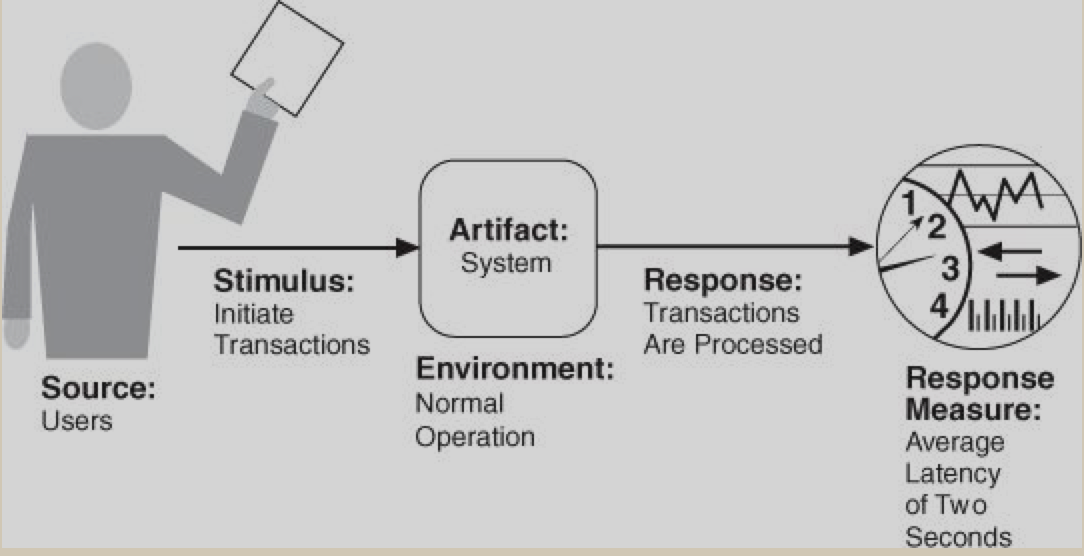
\includegraphics[scale=0.6]{images/sad.png}
\end{center}

We need to say something about the distribution of the arrival of the stimuli.
\begin{itemize}
\item{E.g. The inter-arrival time is always greater than 1.0 secs}
\item{How is this different from the arrival rate is less than 1 per second?}

Any stimulus needs to be processed within 2 seconds of arriving.
The responses should appear in the same order as the stimuli.
\end{itemize}

\subsection{A Possible Architecture}

Queue $\rightarrow$ Process $\rightarrow$ Output

We need to say something about the capacity of the processor:
\begin{itemize}
\item{The worst case processing time for a stimulus is 1.5 seconds best case time is 1.0 secs}
\item{The processor can only process one stimulus at a time.}
We need to say that the queue capacity is 7 stimuli (or some other).
This architecture fails the scenario 

\textbf{Because the arrival rate is greater than the processing rate therefore a queue > 7 is inevitable}
\end{itemize}

\subsection{Performance Tactics}
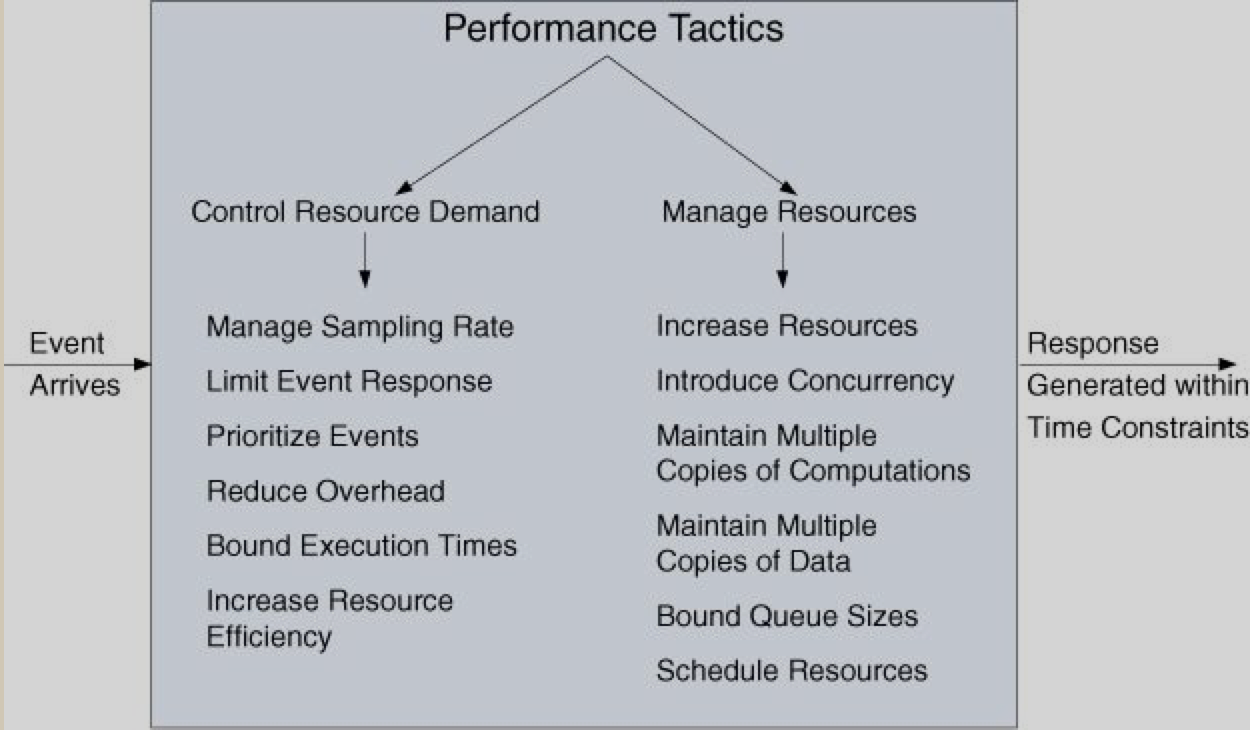
\includegraphics[scale=0.6]{images/zxc.png}

\subsubsection{Control Resource Demand}
\begin{itemize}
  \item
    \textbf{Increase computational efficiency.}
    One step in the processing of an event or a message is applying some
    algorithm.
    Improving the algorithms used in critical areas will decrease latency.
    Sometimes one resource can be traded for another.
    For example, intermediate data may be kept in a
    repository or it may be regenerated depending on time and space resource
    availability.
    This tactic is usually applied to the processor but
    is also effective when applied to other resources such as a disk.
  \item
    \textbf{Reduce computational overhead.}
    If there is no request for a resource, processing needs are reduced.
    In Chapter 17, we will see an example of using Java classes rather than
    Remote Method Invocation (RMI) because the former reduces communication
    requirements.
    The use of intermediaries (so important for modifiability)
    increases the resources consumed in processing an event stream,
    and so removing them improves latency.
    This is a classic modifiability/performance tradeoff.
  \item
    \textbf{Manage event rate.}
    If it is possible to reduce the sampling
    frequency at which environmental variables are monitored,
    demand can be reduced. Sometimes this is possible if the system was
    over engineered.
    Other times an unnecessarily high sampling rate is used
    to establish harmonic periods between multiple streams.\
    That is, some stream or streams of events are oversampled so
    that they can be synchronized.
  \item
    \textbf{Control frequency of sampling.}
    If there is no control over the arrival of externally generated events,
    queued requests can be sampled at a lower frequency,
    possibly resulting in the loss of requests.
  \item
    \textbf{Bound execution times.}
    Place a limit on how much execution time is used to respond to an event.
    Sometimes this makes sense and sometimes it does not.
    For iterative, data-dependent algorithms,
    limiting the number of iterations is a method for bounding execution times.
  \item
    \textbf{Bound queue sizes.}
    This controls the maximum number of queued arrivals and
    consequently the resources used to process the arrivals.
\end{itemize}

\subsubsection{Manage Resources}
\begin{itemize}
  \item
    \textbf{Introduce concurrency.}
    If requests can be processed in parallel, the blocked time can be reduced.
    Concurrency can be introduced by processing different streams of
    events on different threads or by creating additional threads
    to process different sets of activities.
    Once concurrency has been introduced, appropriately allocating
    the threads to resources (load balancing) is important in
    order to maximally exploit the concurrency.
  \item
    \textbf{Maintain multiple copies of either data or computations.}
    Clients in a client-server pattern are replicas of the computation.
    The purpose of replicas is to reduce the contention that would occur
    if all computations took place on a central server.
    Caching is a tactic in which data is replicated,
    either on different speed repositories or on separate repositories,
    to reduce contention.
    Since the data being cached is usually a copy of existing data,
    keeping the copies consistent and synchronized becomes a
    responsibility that the system must assume.
  \item
    \textbf{Increase available resources.}
    Faster processors, additional processors, additional memory,
    and faster networks all have the potential for reducing latency.
    Cost is usually a consideration in the choice of resources,
    but increasing the resources is definitely a tactic to reduce latency.
    This kind of cost/performance trade-off is analysed in Chapter 12.
\end{itemize}

\underline{\textbf{Resource Arbitration}}
\textbf{Scheduling policy.} $\rightarrow$ (FIFO, Fixed-priority, Dynamic priority, Static)

\subsubsection{Control Resource Demand (old version)}
\begin{itemize}
\item{\textbf{Manage the sampling rate} (not always applicable) – ensure you do not have too much to handle.}
\item{\textbf{Limit the event response} – if you are receiving too many events, throw some away.}
\item{\textbf{Prioritize events} – some need a respons in a certain time – some don’t}
\item{\textbf{Reduce overhead} – can you take resource out of handling an event?}
\item{\textbf{Improve the efficiency of processing} – so you can handle more with the same processing}
\end{itemize}

\subsection{Architectural Design Decisions (for performance)}
\begin{itemize}
\item{Allocation of responsibilities}
\item{Coordination model}
\item{Data Model}
\item{Management of resources}
\item{Mapping among architectural elements}
\item{Binding time decisions}
\item{Choice of technology}
\end{itemize}

\subsubsection{Manage Resources}

\begin{itemize}
\item{Increase resources}
\item{Introduce concurrency}
\item{Maintain multiple copies of compute and/or data}
\item{Bound queue sizes}
\item{Schedule resource when there is contention (hard scheduling for highest priority events)}
\end{itemize}

\subsubsection{Allocation of Responsibilities}
\begin{itemize}
\item{Work out areas responsibility of that require heavy resource use to ensure time-critical events take place.}
\item{Work out processing requirements.}
\item{Take account of:
	\begin{itemize}
	\item{Responsibilities arising from threads crossing boundaries of responsibility}
	\item{Responsibilities for thread management}
	\item{Responsibilities for scheduling shared resources}
	\end{itemize}
}
\end{itemize}

\subsubsection{Coordination Model }
\begin{itemize}
\item{What needs to coordinate.}
\item{Is there concurrency?  Ensure it is safe.}
\item{Ensure coordination is appropriate for the style of stimulus.}
\item{Ensure the properties of the coordination model are good for the stimuli and concurrency control?}
\end{itemize}

\subsubsection{Data Model}
\begin{itemize}
\item Determine what parts of the data model will be heavily loaded or have tight time constraints.
\begin{itemize}
\item{Would keeping multiple copies help?}
\item{Would partitioning the data help?}
\item{Is it possible to reduce processing requirements for the data?}
\item{Does adding resource help deal with data bottlenecks?}
\end{itemize}
\end{itemize}

\subsubsection{Mapping Among Architecture Elements }
\begin{itemize}
\item{Does collocation of some components reduce latencies?}
\item{Ensure components with high processing needs are allocated to big processors}
\item{Consider introducing concurrency when you map.}
\item{Consider whether some mappings introduce bottlenecks (e.g. allocating non-interfering tasks to the same thread)}
\end{itemize}

\subsubsection{Resource Management}
\begin{itemize}
\item{Work out what needs high levels of resource}
\item{Ensure these are monitored and managed under all operating modes.}
\item{For example:
\begin{itemize}
\item{Time critical components}
\item{Thread management}
\item{Prioritization}
\item{Locking and scheduling strategies}
\item{Deploying additional resource to meet elevated load.}
\end{itemize}
}
\end{itemize}


\subsubsection{Binding Time}
\begin{itemize}
\item{Look at when you bind.}
\item{Consider the cost of binding at different times.}
\item{Try to avoid performance penalties caused by late binding.}
\end{itemize}

\subsubsection{Choice of Technology}
\begin{itemize}
\item{Is the technology right to let you meet hard deadlines and resource use (e.g. use a real-time OS with proper scheduling).}
\item{You need:
\begin{itemize}
\item{Good scheduling}
\item{Priorities}
\item{Policies for demand reduction}
\item{Allocating processing to tasks}
\item{Other performance-related measurement and management.}
\end{itemize}}
\end{itemize}

\newpage
\section{QA: Security}
We need to consider attacks on \textbf{confidentiality}, \textbf{integrity} and \textbf{availability}. 
Attacks need to be \textbf{monitored} and \textbf{detected} to allow them to be \textbf{resisted where possible}, otherwise we may need some other form of reaction. In the ideal situation we will eventually be able to \textbf{fully recover}.

\subsection{Important Quality Attributes (for security)}
\begin{enumerate}
\item \textbf{Confidentiality} - Only those who should have access are given access
\item \textbf{Integrity} -  Data or services are not subject to unauthorised manipulation.
\item \textbf{Availability} -  The system is available for legitimate use.
\item \textbf{Security Mechanisms} Authentication, Authorisation, non-repudiation
\end{enumerate}

\subsection{General Scenario}
\begin{figure}[h]
\centering 
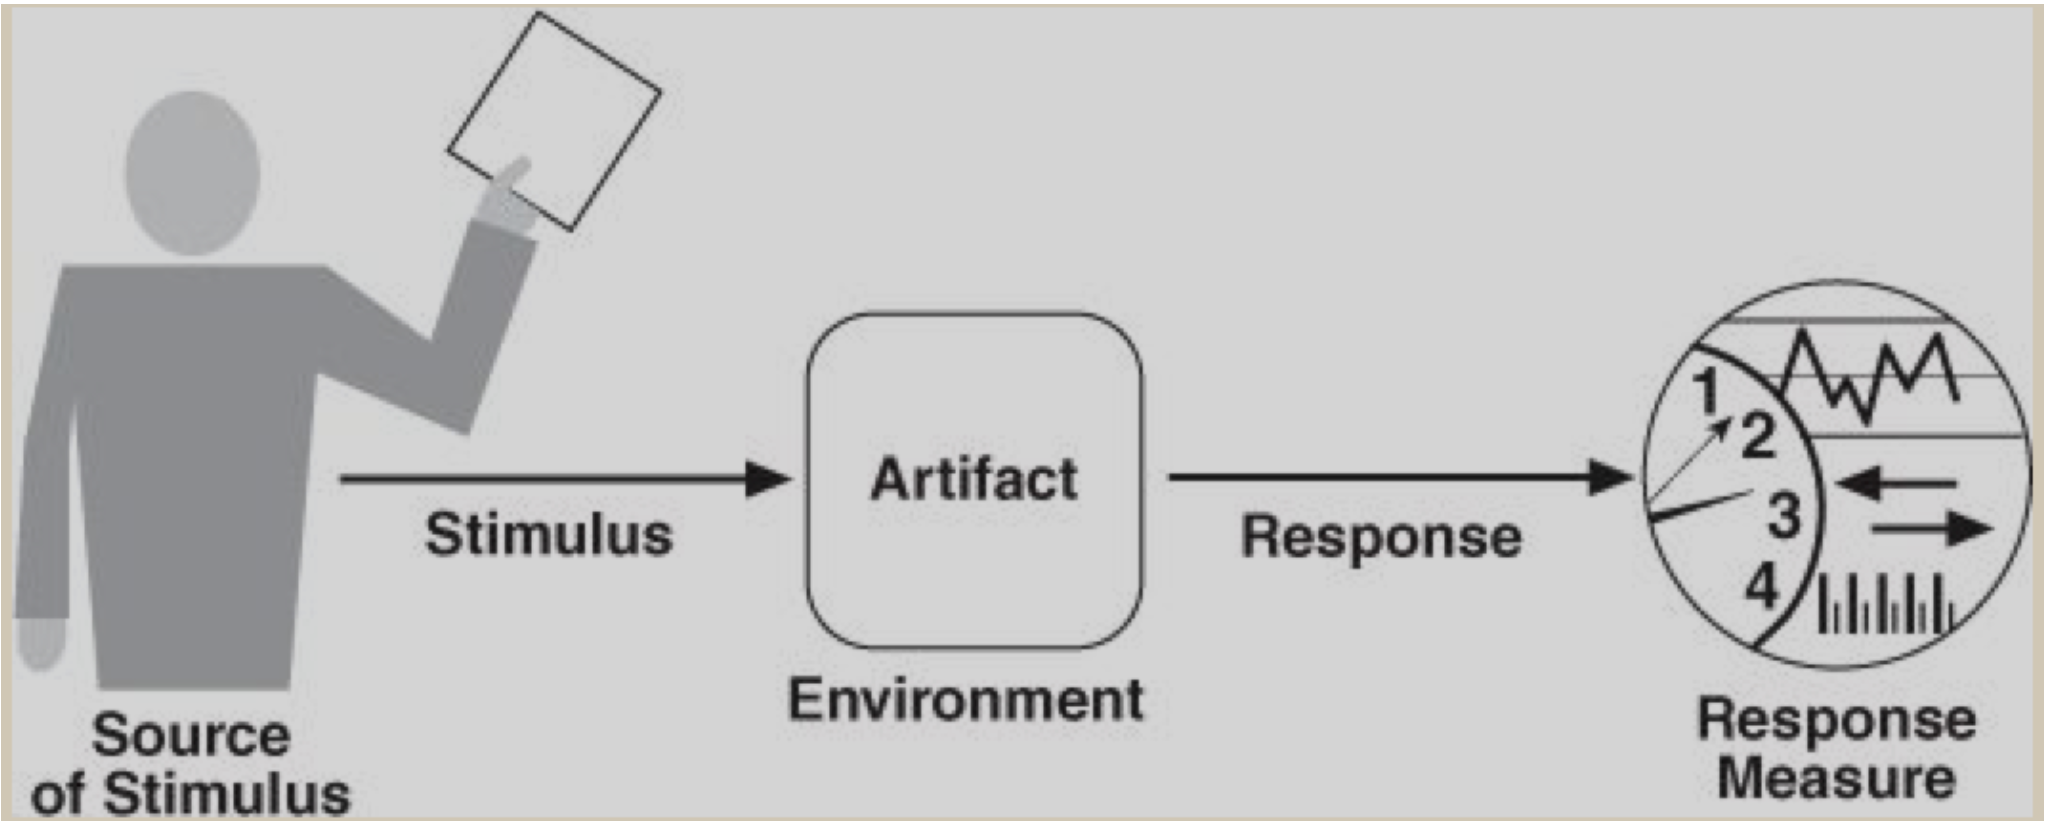
\includegraphics[scale=0.3]{images/genreralqascenario.png}
\end{figure}

\begin{itemize}
\item \textbf{Source} - Humans or systems that may or may not have been identified and can be either inside or outside the organisation
\item \textbf{Stimulus} - Unauthorized attempt to access, manipulate or disable the artifact.
\item \textbf{Artifact} - System services, data, components, data produced or consumed by the system.
\item \textbf{Environment} - online, offline, connected to network, disconnected to network, behind firewall, fully/partially operating, not operational
\item \textbf{Response} - Transaction carried out such that: 
\begin{itemize}
\item Data or services protected from unauthorised access
\item No data manipulation without authorization
\item Parties in a transaction are identified with assurance
\item Parties cannot repudiate their participation
\item Data resources etc ... are available for legitimate use
\item Appropriate people are notified when threat is identified
\end{itemize}
\item \textbf{Response Measure} - assessment of the degree of compromise, temporal and spatial data on the compromise, how many attacks were resisted, how much data is vulnerable
\end{itemize}

\subsection{Concrete Scenario}
Assume a more concrete example of \textbf{Distributed Denial of Service} (DDOS). The components could be:
\begin{itemize}
\item \textbf{Source}- A wide range of systems with different IP.
\item \textbf{Stimulus}- Access to the service provided
\item \textbf{Artifact}- The service we are concerned with
\item \textbf{Environment}- Normal operation
\item \textbf{Response}- Detect Normal Load
\item \textbf{Response Measure}- Mode of operation is changed to ensure normal service to trusted IP addresses (block those doing DDOS)
\end{itemize}

\subsection{Security tactics}
\begin{figure}[H]
\centering 
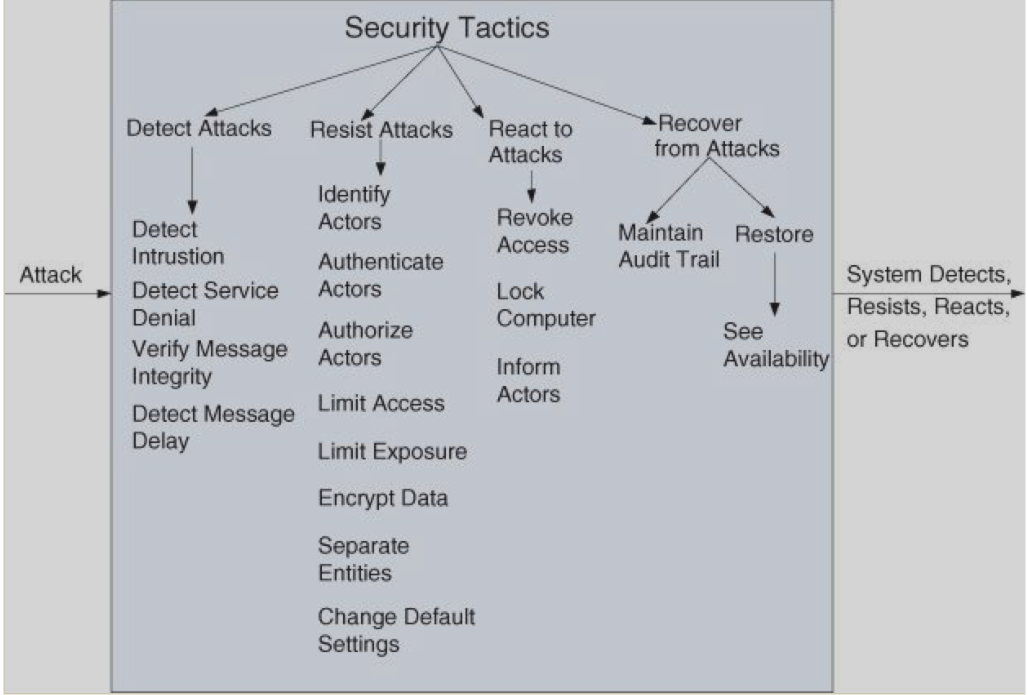
\includegraphics[scale=0.3]{images/security-tactics.png}
\end{figure}

\subsection{Architectural Design Decisions (for security)}
\begin{itemize}
\item{Allocation of responsibilities}
\item{Coordination model}
\item{Data Model}
\item{Management of resources}
\item{Mapping among architectural elements}
\item{Binding time decisions}
\item{Choice of technology}
\end{itemize}
\subsubsection{Manage Resource}
\begin{itemize}
\item Explore the overheads resulting from responsibilities (logging, encryption, recovery etc).
\item Analyse how a user can make demands on a critical resource.
\item Make sure malicious use of resources is detected and managed.
\item Identify and manage the potential for corruption/contamination.
\item Explore the potential for resource use to be used as a covert channel to transmit data.
\item Limit resources used to manage attempts at unauthorised use.
\end{itemize}

\subsubsection{Allocation of Responsibilities}
For security-system responsibilities do the following:
\begin{itemize}
\item Ensure all actors have identities (like roles)
\item Authenticate identities to appropriate actors.
\item Check and Ensure Authorization
\item Ensure Data Encryption
\item Log attempts, successes, failures and other sensitive operations.
\end{itemize}

\subsubsection{Coordination Model}
The following things in the coordination model need to be accounted for:
\begin{itemize}
\item Ensure coordination mechanisms use authentication and 
\item Ensure the coordination model is not vulnerable to tampering, interception, impersonation.
\item The model data involved is encrypted
\item Monitor level of demand for communication to identify excessive demands
\end{itemize}

\subsubsection{Data Model}
\begin{itemize}
\item Ensure there is a valid data model that disallows invalid data flows
\item Ensure logging of access, modification and attempted access or modification
\item Data is protected in flight at rest using appropriate encryption
\item Ensure appropriate backup/recovery mechanisms are in place
\end{itemize}

\subsubsection{Mapping Among Architectural Elements}
\begin{itemize}
\item Explore and be wary how different mappings change the way users can access resources
\item Ensure for all the mappings, the responsibilities (authorization, logging,encryption etc ...) are preserved
\item Ensure recovery from attack is possible
\end{itemize}

\subsubsection{Binding Time}
\begin{itemize}
\item Explore the consequences of varying binding times on the ability to trust actor or components.
\item place mechanisms to ensure trust given in binding time.
\item Explore impact on resource use, capacity/throughput, response time.
\item Ensure the time bindings are ensured with all responsibilities (authorization, logging,encryption etc... )
\item Explore the potential of variation in binding time as a covert channel
\end{itemize}

\subsubsection{Choices of Technologies}
\begin{itemize}
\item  Ensure limitations of technologies are understood and the potential for future compromise is well identified
\item Ensure your chosen technologies support the tactics you want to deploy to protect the system
\end{itemize}

\newpage
\section{QA: Testability}
Testability is concerned with \textbf{ensuring the software architecture eases the work of testers}. The way in which the software is designed should make it easy for \textbf{precise tests} to be developed to measure how successful the software was made.
\begin{itemize}
\item \textbf{Not the same as testing itself}
\item Software architecture is structured in a way so that desired testing can take place
\item Testability is often \textbf{determined by the code structure itself} rather than the connector/component or deployment view
\item Consider the code modules and the dependencies between them that are used to build up the components
\end{itemize}

\subsection{General Scenario}
\begin{itemize}
\item   
   \textbf{Source:}
   Can think of it as who is doing the testing:
   \begin{itemize}
   \item unit testers
   \item integration testers
   \item system testers
   \item acceptance testers
   \item end users
   \end{itemize}
   These tests can be run manually or using automated testing tools
   
\item 
   \textbf{Stimulus:} 
   Why is the set of tests being executed? 
   Could be due to:
   \begin{itemize}
   \item completion of a certain part of the code, or of an entire system
   \item complete integration of subsystem into larger system
   \item completion of entire system
   \item time to deliver the system to the customers
   \end{itemize}
   
    
\item 
   \textbf{Environment:}
   Which environment we are dealing with:
   \begin{itemize}
   \item Design time
   \item Development time
   \item Compile time
   \item Integration time
   \item Deployment time
   \item Run time
   \end{itemize}  

\item
   \textbf{Artifacts:}
   The portion of the system that is being tested

\item 
   \textbf{Response:}
   What is the outcome of running the tests:
   \begin{itemize}
   \item Execute test suite and capture results
   \item Capture activity that resulted in the fault
   \item Control and monitor the state of the system
   \end{itemize} 

\item 
   \textbf{Response Measure:}
   How exactly we will measure the results and if we were successful in the testing
   Could be:
   \begin{itemize}
   \item Find a fault or type of faults
   \item Achieve a certain percentage of code coverage
   \item Time limit for running the tests
   \end{itemize} 
\end{itemize}

\subsection{Concrete Scenario}

\begin{figure}[H]
\begin{center} 
    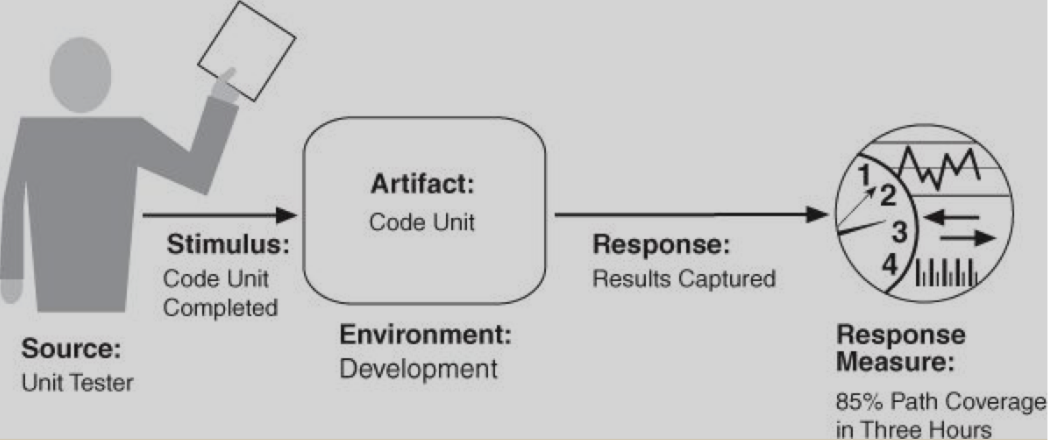
\includegraphics[scale=0.3]{images/testability-concrete.png}
\end{center}
\end{figure}

\begin{itemize}
\item \textbf{Source} - Regression tester
\item \textbf{Stimulus} - Completion of maintenance development to repair a critical bug
\item \textbf{Artifact} - Modules for the full system
\item \textbf{Environment} - Maintenance development
\item \textbf{Response} - Results from path coverage tool
\item \textbf{Response Measure} - Path coverage is better than 95\% of non-looping paths inside modules
\end{itemize}

\subsection{Testability Tactics}
\begin{figure}[H]
\centering 
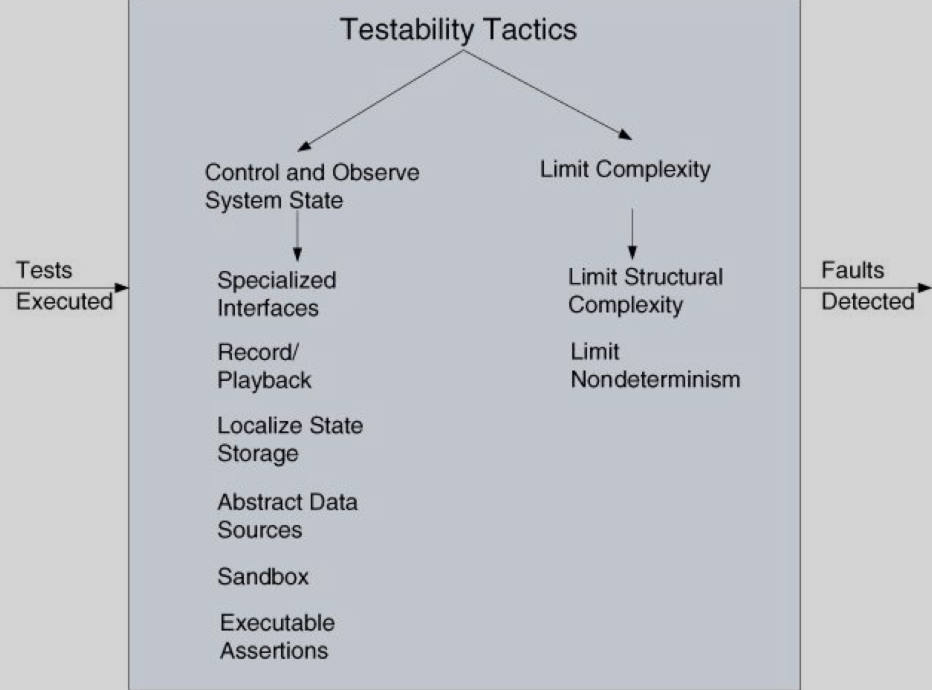
\includegraphics[scale=0.3]{images/testability-tactics.png}
\end{figure}

The goal of tactics for testability is to allow for
easier testing when an increment of software
development has completed. Anything the architect can do to reduce the high
cost of testing will yield a significant benefit. There are two categories of tactics for testability:
\begin{itemize}
\item Adding controllability and observability to the system.
\item Limiting complexity in the system’s design
\end{itemize}

\subsubsection{Category 1 - Control and Observe System State}
\begin{itemize}
\item \textbf{Specialized Interfaces:} to control or capture
variable values for a component either through a
test harness or through normal execution.
\item \textbf{Record/Playback:} capturing information crossing
an interface and using it as input for further
testing.
\item \textbf{Abstract Data Sources:} Abstracting the interfaces
lets you substitute test data more easily. 
\item \textbf{Sandbox:} isolate the system from the real world
to enable experimentation that is unconstrained
by the worry about having to undo the
consequences of the experiment
\item \textbf{Executable Assertions:} assertions are (usually)
hand coded and placed at desired locations to
indicate when and where a program is in a faulty
state - basically when you want to check 

\end{itemize}


\subsubsection{Category 2 - Limit Complexity}
\begin{itemize}
  \item \textbf{Limit Structural Complexity:}  Avoiding or
resolving cyclic dependencies between
components, isolating and encapsulating
dependencies on the external environment,
and reducing dependencies between
components in general.
\item \textbf{Limit Non-determinism:} finding all the sources
of non-determinism, such as unconstrained
parallelism, and weeding them out as far as
possible.
\end{itemize}

\subsection{Architectural Design Descisions (for testability)}
\textit{During testing, tester has to control and observe the state of the system.}
\begin{itemize}
\item{Allocation of responsibilities}
\item{Coordination model}
\item{Data Model}
\item{Management of resources}
\item{Mapping among architectural elements}
\item{Binding time decisions}
\item{Choice of technology}
\end{itemize}

\subsubsection{Allocation of responsibilities}
This means determining which system responsibilities are most critical and thus need the most testing.
Make sure that system responsibilities have been created to actually perform the testing and capture the results, capture (log) activity that resulted in fault or unexpected behaviour, control and observe relevant system state for testing.

\subsubsection{Coordination Model}
Ensure system's coordination and communication mechanisms support the execution of the test suite, support capturing activity that resulted in a fault, support injection and monitoring of state, and do not introduce necessary non-determinism

\subsubsection{Data Model}
Determine the major data abstractions that must be tested to ensure the correct operation of the system.

\subsubsection{Mapping Among Architectural Elements}
Determine how to test possible mappings of architectural elements so that the desired test response is achieved.

\subsubsection{Resource Management}
Ensure that there are sufficient resources available to execute the test suite and capture the results. 
Ensure test environment is representative of the environment in which the system will run in.

\subsubsection{Binding Time}
Ensure that components that are bound later than compile time can be tested in the late-bound context.

\subsubsection{Choice of Technology}
Determine what technologies are available to help achieve the testability scenarios that apply to your architecture.

\subsection{Summary}
Testability becomes increasingly important in an environment where development is test driven. The main ways we can improve testability is via changing the observability of phenomena or by limiting complexity.

\newpage
\section{QA: Modifiability}
Modifiability is concerned with \textbf{how easy it is to make changes to the system} if this is required. 
\textit{So, for example, having a lot of hard coded values would not make a system very modifiable.}

It's not about the actual modifying but with how easy it would be to do the modifying.
\textbf{It is very important for a system to be modifiable because changes can be very costly to make.}

\subsection{Four key questions that are asked when making a system:}
1)   What can change?\newline
2)   How likely is something to change?\newline
3)   When, where, how, and by whom will the change be made?\newline
4)   What is the cost of making these changes? \newline

\subsection{General Scenario}
\hskip-3.0cm\begin{figure}[H] 
    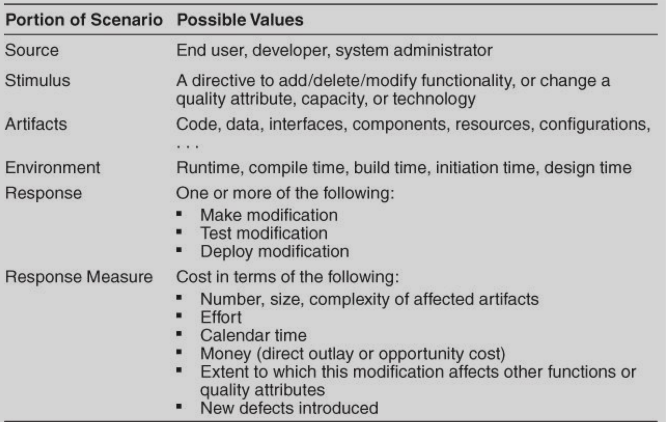
\includegraphics[scale=0.7]{images/modifiability-general.png}
\end{figure}

\subsection{Concrete Scenario}
\begin{figure}[H]
\begin{center} 
    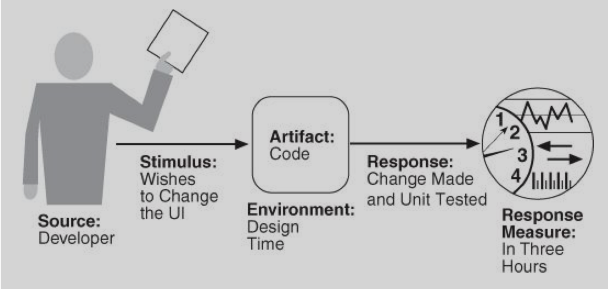
\includegraphics[scale=0.5]{images/modifiability-concrete.png}
\end{center}
\end{figure}

\begin{itemize}
\item Source: Developer
\item Stimulus: Wishes to change the UI
\item Artifact: The code itself
\item Environment: Design time
\item Response: Change made and unit tested
\item Response Measure: This should all be done in 3 hours
\end{itemize}

\subsection{Modifiability Tactics}
\begin{figure}[H]
\centering 
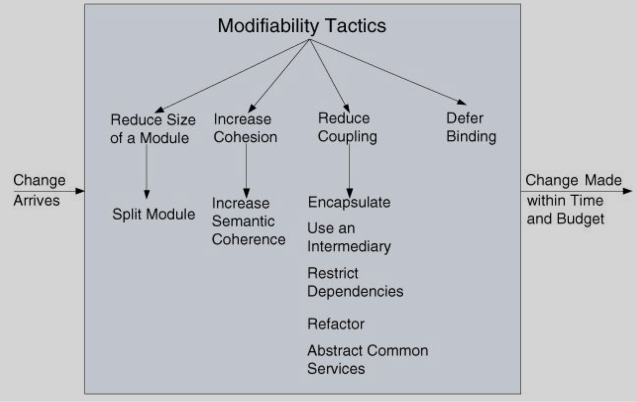
\includegraphics[scale=0.6]{images/modifiability-tactics.png}
\end{figure}

\subsubsection{Important Terms}
\begin{itemize}
\item \textbf{Cohesion -} refers to the degree to which the elements inside a module belong together.
\item \textbf{Semantic coherence –} all the responsibilities in a layer work together without too much reliance on other layers
\item \textbf{Coupling –} degree of interdependence between software modules
\item \textbf{Intermediary -} a program or set of programs that in some way evaluates, filters, modifies, or otherwise interjects some function between two end users or end-use programs
\item \textbf{Binding -} generally refers to a mapping of one thing to another. In the context of software libraries, bindings are wrapper libraries that bridge two programming languages, so that a library written for one language can be used in another language.
\item \textbf{Deferred Binding -} When a modification is made by the developer, there is usually a testing and distribution process that determines the time lag between the making of the change and the availability of that change to the end user. Binding at runtime means that the system has been prepared for that binding and all of the testing and distribution steps have been completed. Deferring binding time also supports allowing the end user or system administrator to make settings or provide input that affects behaviour.
\end{itemize}

\subsubsection{Tactics of Modifiability}
\begin{itemize}
  \item \textbf{Reduce size of a module} – split it up
  \item \textbf{Increase cohesion within a module} – increase semantic coherence
  \item \textbf{Decrease the coupling in the module} – this can be done in the following ways:
   \begin{itemize}
   \item Encapsulate
   \item Use an intermediary
   \item Restrict dependencies
   \item Refactor
   \item Abstract common servies – think of OOP
   \end{itemize}
   \item \textbf{Defer binding} – we can use the “reduce coupling” tactics later in the process so that they   are more likely to be done by a computer rather than a human
\end{itemize}

\subsection{Architectural Design Decisions (for modifiability)}
\begin{itemize}
\item{Allocation of responsibilities}
\item{Coordination model}
\item{Data Model}
\item{Management of resources}
\item{Mapping among architectural elements}
\item{Binding time decisions}
\item{Choice of technology}
\end{itemize}

\subsubsection{Allocation of Responsibilities}
Try to work out how things are likely to change, work out what responsibilities change.
Try to modularize so that change does not affect responsibilities that span many modules.

\subsubsection{Coordination Model}
See how changes are likely to affect coordination and make it so that most probable changes impact coordination across a small number of modules.  

\subsubsection{Data Model}
Data model changes impact as few modules as possible.

\subsubsection{Mapping Among Architectural Elements}
Look at potential changes and see if some may best be responded to by changing the mapping to elements.

\subsubsection{Resource Management}
Determine how a change in responsibility will change resource.

\subsubsection{Binding Time}
Control choice of binding times so there are not too many combinations to consider. Defer binding to later.

\subsubsection{Choice of Technology} 
Choose technologies that make the most likely changes easier – of course, balance with costs.


\subsection{Summary}
Summary:
For better modifiability:
1) Improve cohesion, reduce coupling
2) Use mechanisms that allow you to introduce change late in development cycle
3) Of course, take the cost of all these mechanisms into account

\newpage
\section{Connectors}

\textbf{Software connectors} are key elements of the software's architecture. They define the rules of \textbf{interaction} between \textbf{components}. There are various levels of software connectors that range from \textit{simple} to \textit{complex} connections.
\begin{itemize}
\item Simple: shared variable access, method calls ...
\item Complex: database access, client-server, scheduler, load balancer ...\\
\end{itemize}

In a projects \textbf{code base} the connections between components are often implicit and can be noticed easily. In the architecture design we \textbf{explicitly identify} them, to allow us to capture \textbf{system interactions} (at the level of the components). The specification for interactions are often \textit{complex.} An example for \textbf{LinkedIn} is provided below:\\

% IMAGE: LinkedIn Data
\begin{figure}[H]
\centering
\hskip-2.5cm\begin{subfigure}{1\textwidth}
  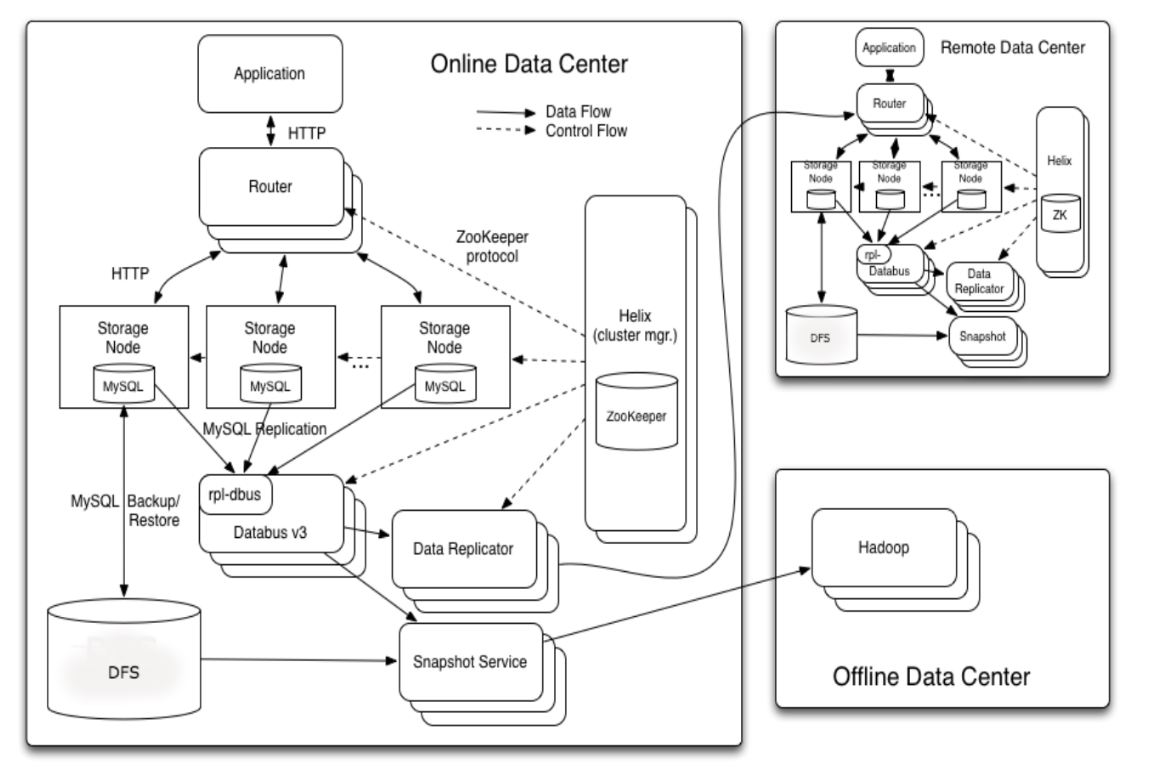
\includegraphics[width=1\linewidth]
  {images/10-linked.png}
\end{subfigure}
%\caption{-}
\end{figure}

% IMAGE: LinkedIn Redliner
\begin{figure}[H]
\centering
\hskip-2.5cm\begin{subfigure}{1\textwidth}
  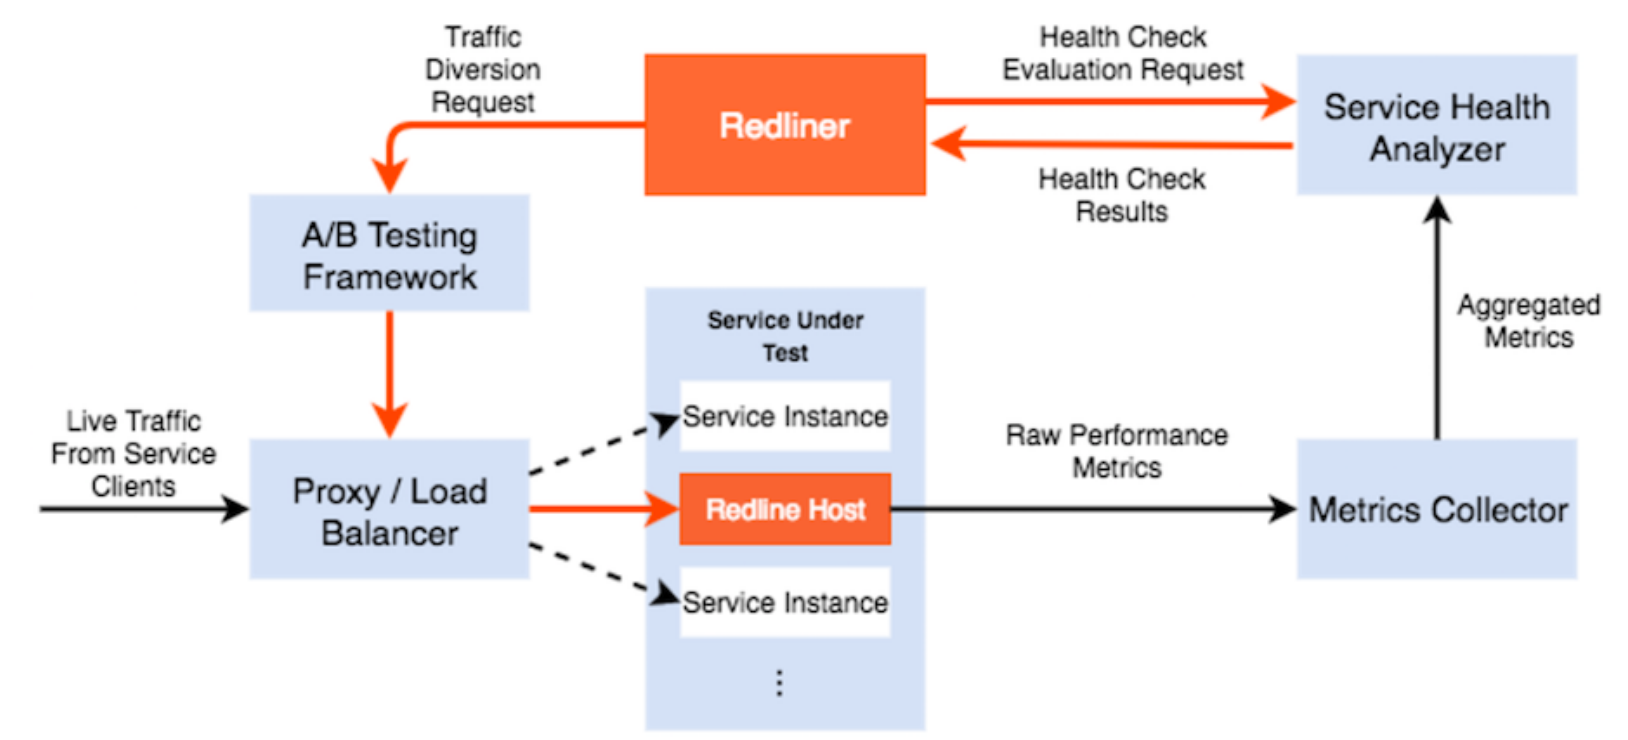
\includegraphics[width=1\linewidth]
  {images/10-linked-redliner.png}
\end{subfigure}
%\caption{-}
\end{figure}

\subsection{What is Different About Connectors?}
Depending on the software project, \textbf{components} will have \textbf{application-specific} functionality. \textbf{Connectors} provide \textit{interaction mechanisms} that are \textit{generic} across different application. \textbf{Interaction} may involve \textbf{multiple components}, and may have a protocol associated to it.\\

\subsection{Benefits of Explicit Connectors}
\begin{itemize}
\item \textbf{Interaction} is defined by the arrangement of the connectors (as far as possible)
\item \textbf{Component interaction} is defined by the pattern of connectors in the architecture
\item \textbf{Interaction} is \textit{"independent"} of the components
\end{itemize}

\subsection{Roles Played By Software Connectors}
The specification of the connector protocols determine:
\begin{itemize}
\item The types of interfaces
\item Properties of interaction
\item Riles about ordering interaction
\item Measurable features of interactions\\
\end{itemize}

Connectors often have multiple roles, the main roles are:
\begin{itemize}
\item Communication
\item Coordination
\item Conversion
\item Facilitation
\end{itemize}

\subsection{Communication}
Information is transmitted between \textbf{components} (e.g. message passing; method calls). \textbf{Connectors} constrain:
\begin{itemize}
\item \textbf{Direction of flow }(The pipes in the image below)
\item \textbf{Capacity / rate of flow}\\
\end{itemize}

** Additional Information **
\begin{itemize}
\item Connector providing communication services support \textbf{transmission} of data among components
\item Data transfer services are a primary building block of component interaction
\item Components routinely pass messages, exchange data to be processed and communication results of computations
\end{itemize}

% IMAGE: Pipes
\begin{figure}[H]
\centering
\hskip-2.5cm\begin{subfigure}{1\textwidth}
  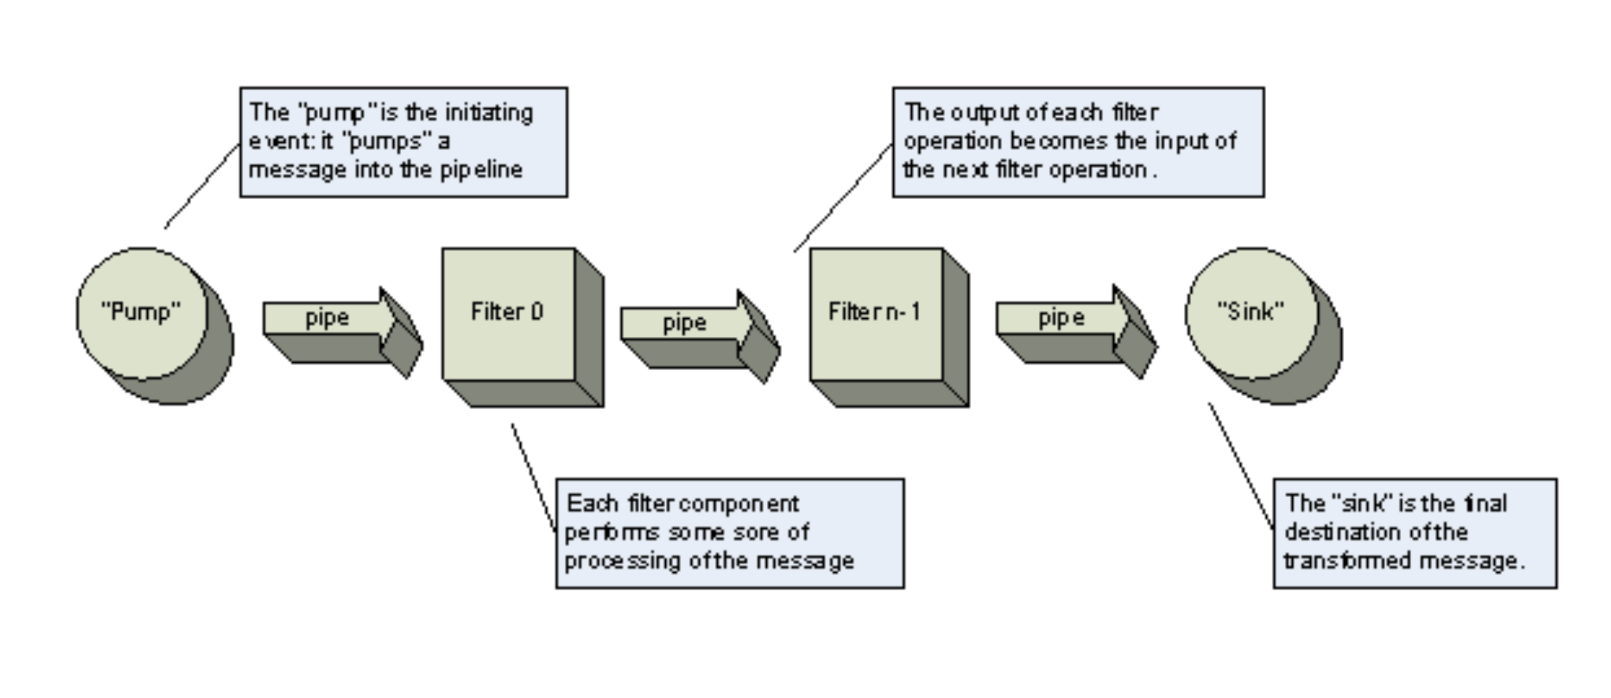
\includegraphics[width=1\linewidth]
  {images/10-pipes.png}
\end{subfigure}
%\caption{-}
\end{figure}

Connectors influence measurable quality attributes of the system. It separates \textbf{communication} from functional aspects.
\subsection{Coordination}
\textbf{Coordination} controls the timing \textbf{relationship} of the functional aspects of the system. \\

** Additional Information ** 
\begin{itemize}
\item Connectors providing coordination services support transfer of \textbf{control} among components
\item Components interact by passing the thread of execution to each other
\item \textbf{Function calls and method invocations are examples of coordination connectors}
\item Higher-order connectors, such as signals and load balancing connectors provide richer, more complex interaction built and coordination services
\end{itemize}

\subsection{Conversion}
\textbf{Conversion} is how to get components to interact that \textbf{do not} have the right means of interaction. \textbf{Incompatibilities} might be related to: datatypes, ordering, frequency, structure of parameters etc ...\\

Examples of types of converters:
\begin{itemize}
\item Wrappers: deal with structural issues
\item Adaptors: deal with datatype incompatibilities\\
\end{itemize}

** Additional Information **
\begin{itemize}
\item Connectors providing conversion services \textbf{transform the interaction} required by one component to that provided by another
\item Enabling heterogeneous components to interact with each other is \textbf{not} a trivial task
\item Conversion services allow components that have not been specifically tailored for each other to establish and conduct interaction
\end{itemize}

\subsection{Facilitation}
\textbf{Facilitation} enables interaction among a group of components that are intended to interact with one and other.

** Additional Information ** 
\begin{itemize}
\item Improve interaction of components that were intended to interoperate (usually \textbf{optimise} or streamlines interactions)
\item Ensure proper performance profiles (load balancing or scheduling)
\item Synchronization mechanisms (monitors $\rightarrow$ enforce mutex access to resources)
\end{itemize}

\subsection{Types of Connectors (Talyor, Medvidovic \& Dashofy)}
\begin{table}[H]
\begin{tabular}{|l|p{10cm}|}
\hline
Connector & Description\\
\hline
Method/Procedure Call & Producre call connectors model the flow of control among components through various invocation techniques. They are thus \textbf{coordination connector}. [Examples: fork and exec]\\
\hline
Data Access & Data access connectors allow components to access maintained by a data store component. Therefore they provide \textbf{communication services}. [Example: JDBC $\rightarrow$ java SQL driver]\\
\hline
Event & An even as the instantaneous effect of the termination of the invocation of an operation on an object, which occurs at that object's location. [Example: windows with GUI inputs] \\
\hline
Stream & Streams are used to preform transfer of large amounts of data between autonomous processes. Thus they provide \textbf{communication services} in a system. [Examples: UNIX pipes, TCP/UDP sockets, client-server protocols]\\
\hline
Distributor & Distributor connectors perform the identification of interaction paths and subsequent routing of communication and coordination information among components along these paths. They provide \textbf{facilitation} services. \textit{[Distributor connectos never exist by themselves, but provide assistance to other connectors, such as steams or procedure calls)}\\
\hline
Arbitrator & When components are aware of the presence of other components but cannot make assumptions about their needs and state, arbitrators streamline system operation and resolve any conflicts (providing \textbf{facilitation}). They also redirect the flow of control (providing \textbf{coordination}) \\
\hline
Adaptor & Adaptor connectors provide facilities to support interaction between components that have not been designed to interoperate. \textit{(adopters involve matching communication polices and interaction protocols among components, thus providing \textbf{conversion} services.}\\
\hline
\end{tabular}
\end{table}
\newpage
\section{Architectural Patterns}
An architectural pattern is a general, reusable solution to a
commonly occurring problem in software architecture within a
given context.

It comprises of:
\begin{itemize}
\item
  \textbf{Context} that provides a frame for a problem.
\item
  \textbf{Problem} that is a generalized description of a class of problems with
  QA requirements that need to be met.
\item
  \textbf{Solution} that is suitably generalized in the same way as the problem.
\end{itemize}


We consider:
\begin{itemize}
\item
  \textbf{Static Patterns} designed to solve issues around development and maintenance of
  the code bae.
\item
  \textbf{Connector and component models} that consider patterns of interaction,
  monitoring at runtime and responses to stimuli.
\item
  \textbf{Deployment patterns} that consider the allocation of elements to hardware
  resources and the availability of resources in the system.
\end{itemize}

\subsection{Static Patterns}
\subsubsection{Layer Pattern}

Description:
% IMAGE: Pipes
\begin{figure}[H]
\centering
  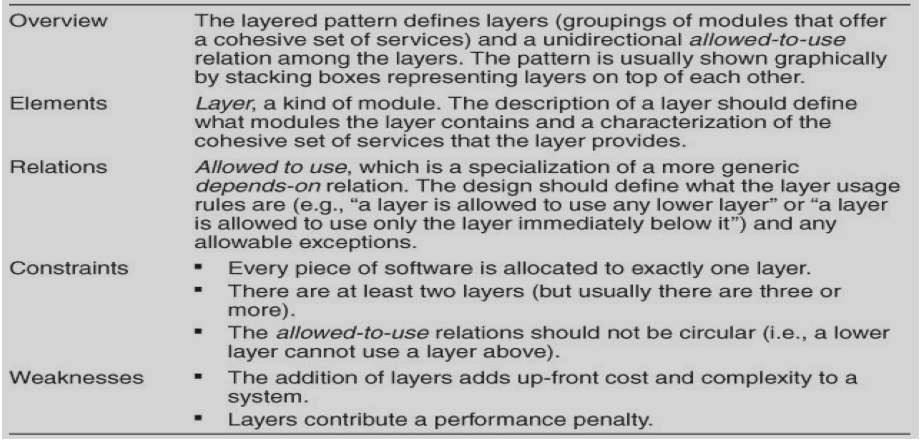
\includegraphics[width=1\linewidth]{images/layered.png}
%\caption{-}
\end{figure}


In a logical multilayered architecture for an
information system with an object-oriented design,
the following four are the most common:

\begin{itemize}
\item
  Presentation layer (a.k.a UI layer, view layer ...)
\item
  Application layer (a.k.a service layer)
\item
  Business layer (a.k.a business logical layer (BLL), domain layer)
\item
  Data access layer (a.k.a persistence layer, logging, networking, database)
\end{itemize}

% IMAGE: Pipes
\begin{figure}[H]
\centering
  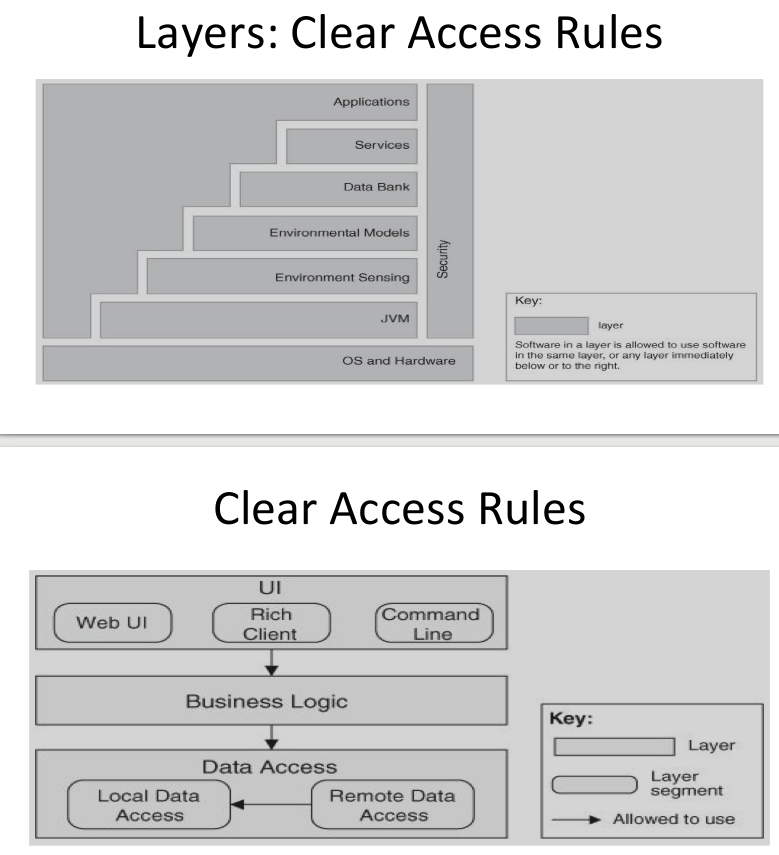
\includegraphics[width=1\linewidth]
  {images/access_rules.png}
%\caption{-}
\end{figure}

\subsection{Connector and component models}

\subsubsection{Model-View-Controller}

\textbf{Context}: The user interface is subject to continuing change to either
meet the needs of the application or diversity in the user group.

\textbf{Problem}:
\begin{itemize}
\item
  Isolating the UI functionality from the Application functionality.
\item
  Maintaining multiple views in the presence of change in the underlying data.
\end{itemize}


% IMAGE: Pipes
\begin{figure}[H]
\centering
  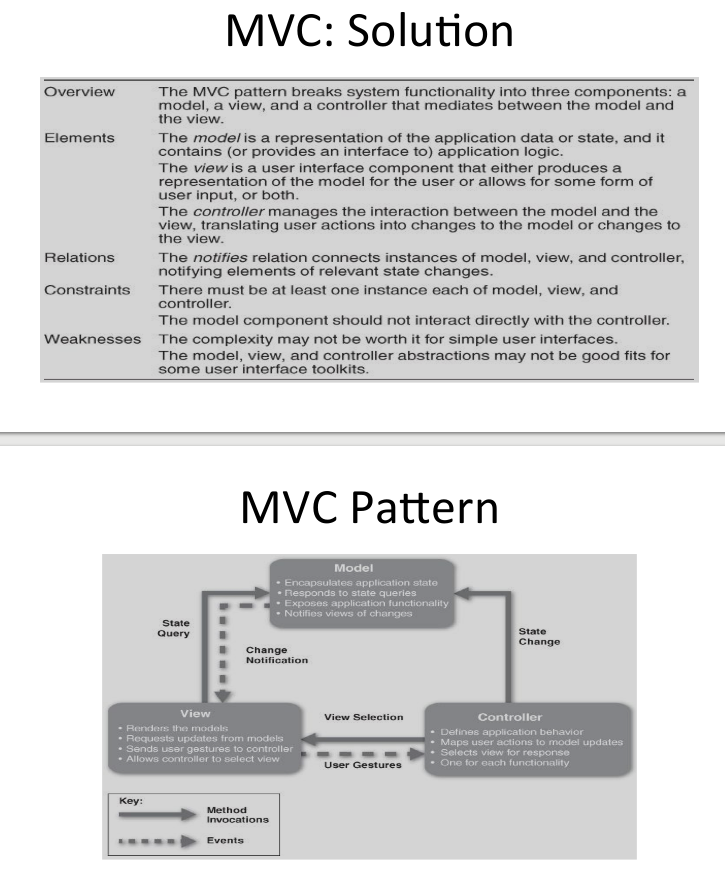
\includegraphics[width=1\linewidth]
  {images/mvc.png}
%\caption{-}
\end{figure}

\subsection{Deployment/Allocation patterns}

% Context:
% \begin{itemize}
% \item
%   We are concerned with resource use.
% \item
%   We consider flexible deployment of resource.
% \item
%   the QAs we care about are sensitive to the pattern of deployment and the use
%   of resources.
% \end{itemize}

\subsubsection{Map-reduce pattern}

Context:
\begin{itemize}
\item
  We have large quantities of data that we want to process in parallel.
\item
  This encourages an approach that involves significant amounts of independent processing.
\end{itemize}

% IMAGE: Pipes
\begin{figure}[H]
\centering
  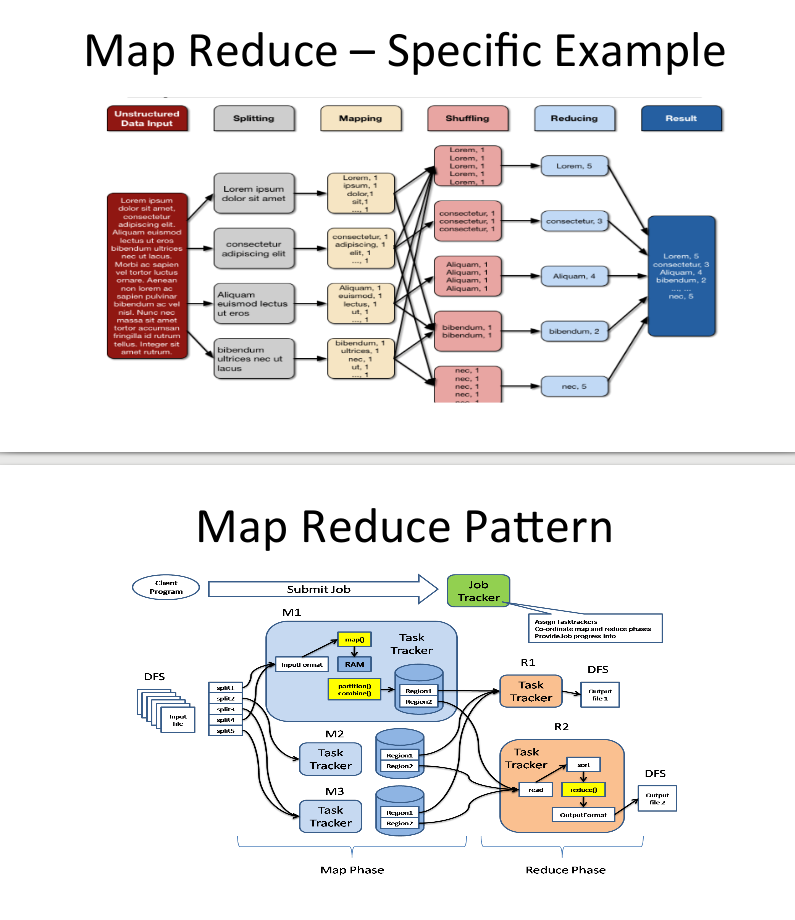
\includegraphics[width=1\linewidth]
  {images/mapreduce.png}
%\caption{-}
\end{figure}

\subsubsection{Other Allocation Patterns}

\begin{itemize}
\item
  Multi-tier architecture pattern
\item
  Cloud architectures
\end{itemize}

\subsection{Other patterns}
\begin{itemize}
\item
  Pipe and Filter Pattern
\item
  Broker Pattern
\item
  Client-Server Pattern
\item
  Peer-to-Peer Pattern
\item
  Service-Oriented Architecture Pattern
\item
  Publish-Subscribe Pattern
\item
  Shared Data Pattern
\end{itemize}
\subsubsection{Pipe and Filter Pattern}
\begin{itemize}
\item  It consists of any number of components (filters) that transform or filter data, before passing it on via connectors (pipes) to other components.
\item The filter transforms or filters the data it receives via the pipes with which it is connected. A filter can have any number of input pipes and any number of output pipes.
\item The pipe is the connector that passes data from one filter to the next. It is a directional stream of data, that is usually implemented by a data buffer to store all data, until the next filter has time to process it.
\item This architecture is great if you have a lot of transformations to perform and you need to be very flexible in using them, yet you want them to be robust.
\item amazing for parallelisation 
\end{itemize}
\begin{figure}[h]
\centering 
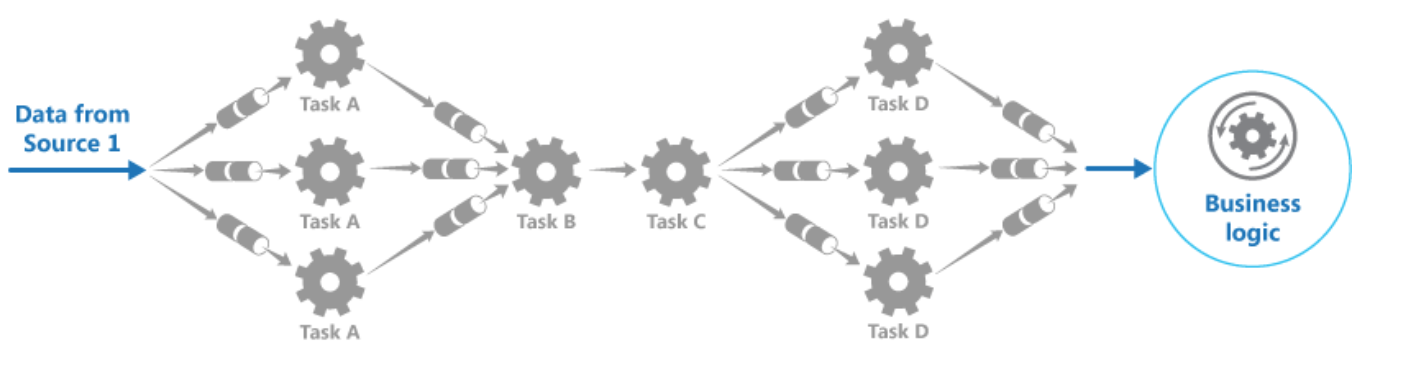
\includegraphics[scale=0.6]{images/pnf.png}
\end{figure}

\subsubsection{Broker Pattern}
\begin{itemize}
\item The Broker architectural pattern can be used to structure distributed software systems with decoupled components that interact by remote service invocations. A broker component is responsible for coordinating communication, such as forwarding requests, as well as for transmitting results and exceptions.
\item Makes communication among remote and heterogeneous classes easy.
\item Keep in mind this is not very scalable, so it loses effectiveness for larger systems.
\end{itemize}

\subsubsection{Client-Server Pattern}
\begin{itemize}
\item The client–server model is a distributed application structure that partitions tasks or workloads between the providers of a resource or service, called servers, and service requesters, called clients. Often clients and servers communicate over a computer network on separate hardware, but both client and server may reside in the same system. A server host runs one or more server programs which share their resources with clients.

\begin{figure}[h]
\centering 
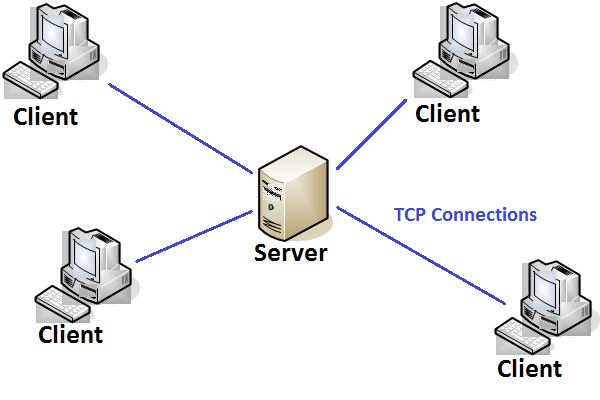
\includegraphics[scale=0.5]{images/client_server.png}
\end{figure}

\item The computing power, memory and storage requirements of a server must be scaled appropriately to the expected work load.

\end{itemize}
\subsubsection{Peer-to-peer pattern}
\begin{itemize}
\item Peer-to-peer (P2P) computing or networking is a distributed application architecture that partitions tasks or workloads between peers. Peers are equally privileged, equipotent participants in the application. They are said to form a peer-to-peer network of nodes.
\end{itemize}

\begin{figure}[h]
\centering 
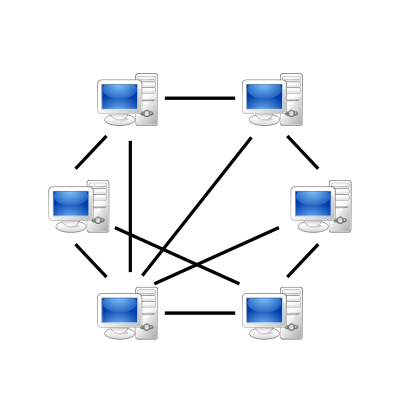
\includegraphics[scale=0.5]{images/p2p.png}
\end{figure}

\begin{figure}[h]
\centering 
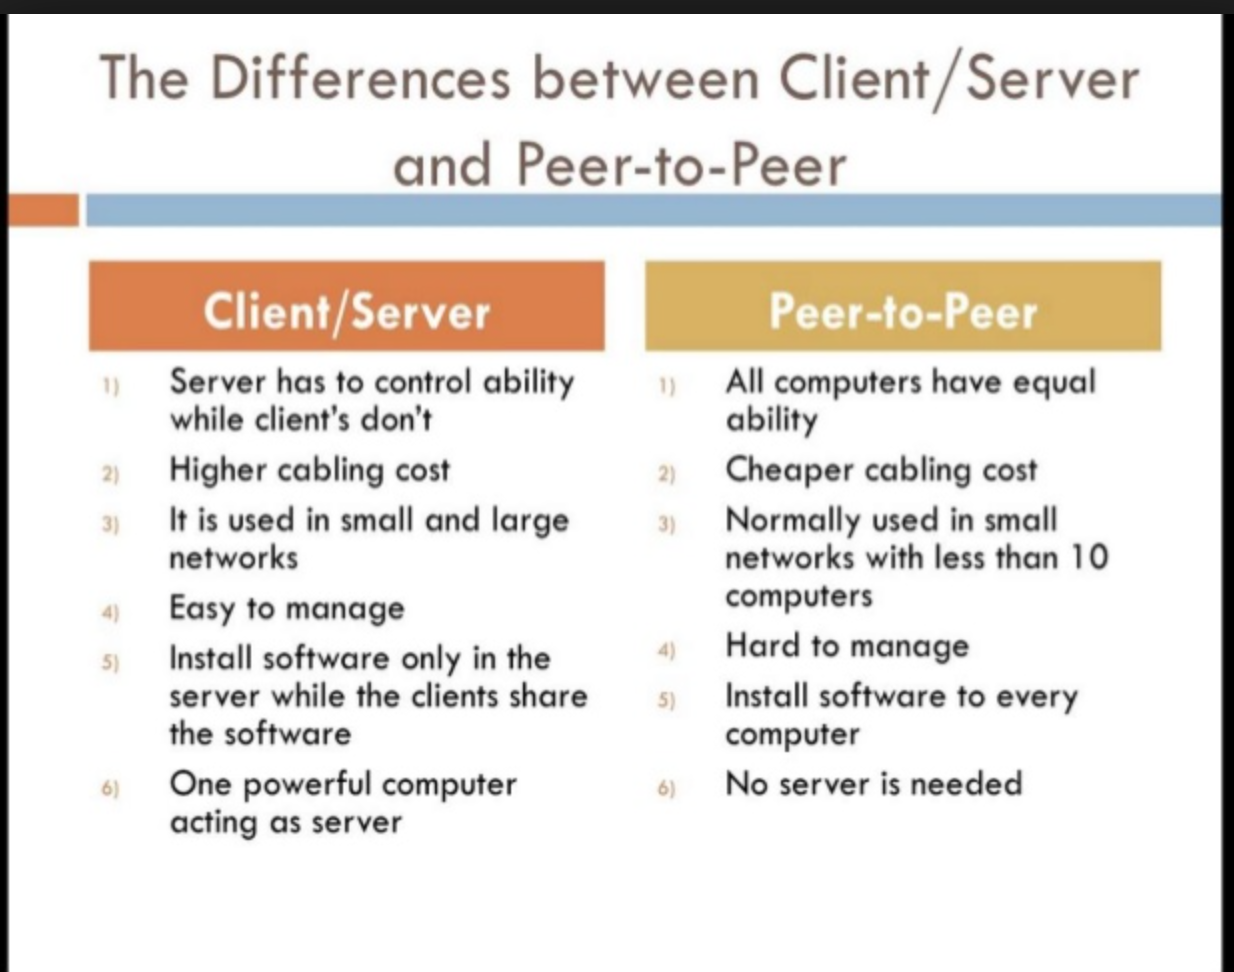
\includegraphics[scale=0.5]{images/csvsp2p.png}
\end{figure}


\subsubsection{Service Oriented Architecture Pattern}
A service-oriented architecture (SOA) is a style of software design where services are provided to the other components by application components, through a communication protocol over a network. The basic principles of service oriented architecture are independent of vendors, products and technologies. A service is a discrete unit of functionality that can be accessed remotely and acted upon and updated independently, such as retrieving a credit card statement online.

\textbf{Properties}:
\begin{enumerate}
\item It logically represents a business activity with a specified outcome.
\item It is self-contained.
\item It is a black box for its consumers.
\item it may consist of other underlying services.
\item loose coupling between services
\end{enumerate}

\textbf{Defining concepts}
\begin{enumerate}
\item Business value is given more importance than technical strategy.
\item Strategic goals are given more importance than project-specific benefits.
\item Intrinsic inter-operability is given more importance than custom integration.
\item Shared services are given more importance than specific-purpose implementations.
\item Flexibility is given more importance than optimization.
\item Evolutionary refinement is given more importance than pursuit of initial perfection.
\end{enumerate}

\subsubsection{Publish Subscribe Pattern}
publish–subscribe is a messaging pattern where senders of messages, called publishers, do not program the messages to be sent directly to specific receivers, called subscribers, but instead characterize published messages into classes without knowledge of which subscribers, if any, there may be. Similarly, subscribers express interest in one or more classes and only receive messages that are of interest, without knowledge of which publishers, if any, there are.

\textbf{Properties}
\begin{enumerate}
\item Loose coupling between publishers and subscribers- can be both an advantage and disadvantage
\item better scalability that client server as parallel operation possible.
\end{enumerate}

\subsubsection{Shared Data Pattern}
\begin{enumerate}
\item intent is to Decouple the production of data from their consumption.
\item Consider the case of an application built as a collection of components. These components interact by exchanging data. In a data exchange, the component that generates the data is called the data producer and the component that receives the data is called the data consumer.Data pools are introduced to act as shared memory areas through which data are exchanged among application components. The data pools physically contain the data items. The producers of data deposit the data into the data pool and the consumers of data retrieve the data they need from the data poo

\end{enumerate}


\begin{figure}[h]
\centering 
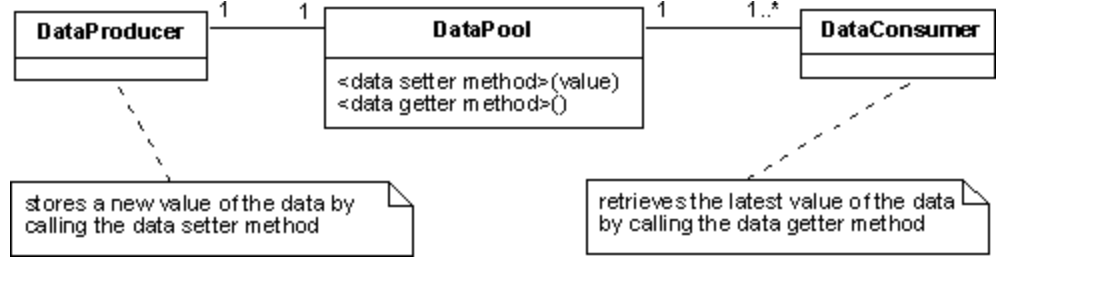
\includegraphics[scale=0.8]{images/shareddata.png}
\end{figure}

\subsection{Relationship between Patterns and Tactics}

% IMAGE: Pipes
\begin{figure}[H]
\centering
  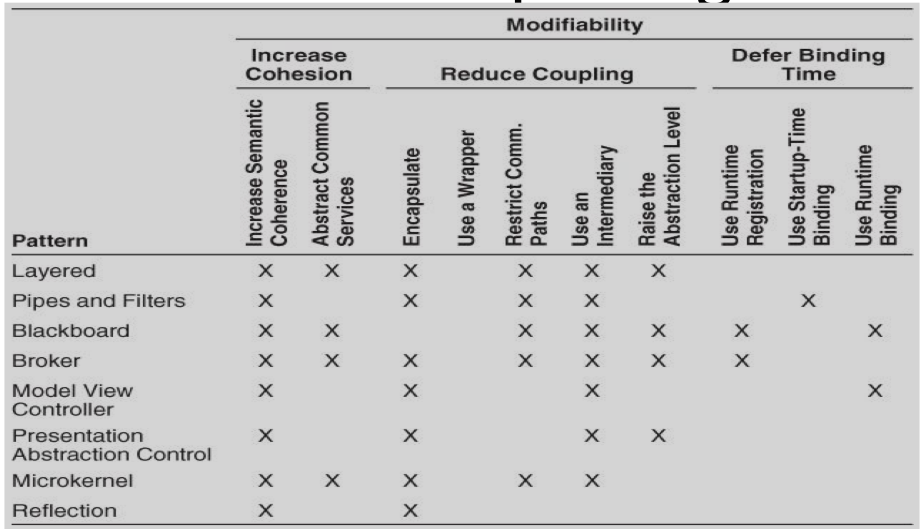
\includegraphics[width=1\linewidth]
  {images/relationship.png}
%\caption{-}
\end{figure}

\newpage
\section{Architectural Modelling}
When building a software architecture, we want to ideally have control over the quality attributes (example – testability, modifiability, etc) and even to be able to predict how well our system will be able to do in each one in advance. 

So – we want to be able to build a predictive model of the software architecture and then use this model to predict the quality attributes – how well our software will perform on each of them.

\subsection{How the model looks like:}
1)  The beginning specifies the distribution of arrivals of service requests. \newline
2)  The queuing discipline \newline
3)  The scheduling algorithm  \newline
4)  Routing of messages coming from the algorithm  \newline
5)  The results – could be the quality attributes the model is predicting \newline

\subsection{MVC Model – model to test the “performance” quality attribute}
1) The view component will service the service requests at some rate.  \newline
2) The view translates these into service requests for the controller.  \newline
3) The there are service requests from the controller to the view, from the controller to the model, and from the model to the view component – all are interleaved.  \newline

If we have good estimates for all the different components of the model (distribution of external service demands, queuing disciplines, network latencies, transfer characteristics), then it can be a very good predictor of quality attributes.

\subsection{Main Quality Attributes and their Analysis Techniques}
The main quality attributes and their analysis techniques are:
\begin{itemize}

\item \textbf{Availability} – Markov models, statistical models \newline
Availability is a measure of software quality defined as MTBF / (MTBF + MTTR)
MTBF is Mean Time Between Failures
MTTR is Mean Time To Repair 

\item \textbf{Interoperability} – Conceptual framework 

\item \textbf{Modifiability} – Coupling and cohesion metrics, cost models

\item \textbf{Performance} – Queuing theory, real-time scheduling theory

\item \textbf{Security} – No architectural models

\item \textbf{Testability} – Component interaction metrics

\item \textbf{Usability} – No architectural models
\end{itemize}

Some QAs have good, well established analysis techniques, others do not,

\subsection{Types of Analysis}
\begin{itemize}
\item
\textbf{Thought experiment:} just a sort of discussion using informed people. 

\item
\textbf{Back of the envelope:} using very approximate techniques with unreliable assumptions

\item
\textbf{Checklist:} collated experience.

\item
\textbf{Analytic Model:} based on sound abstractions –heavily dependent on estimates being correct

\item
\textbf{Simulation:} higher level of detail – less analytic, more concrete 

\item
\textbf{Prototype:} approximate system in an experimental setup

\item
\textbf{Experiment:} fielded system, simulated load 

\item
\textbf{Instrumentation:} measuring the variable of interest
\end{itemize}

\subsection{Summary}
Architecture is the correct level to deal with quality attributes.
Analysis can be costly, depending on how accurate you want it to be.
Analysis throughout the lifecycle helps with decision taking.

\newpage
\section{The Life-cycle}
They impose some discipline on the development process – order stages and activities of the development process. Usually it's an ongoing process improvement cycle that focuses on making this process better.

\subsection{Typical Examples}
There are some typical stages of the software lifecycle.
\begin{figure}[H]
\begin{center} 
    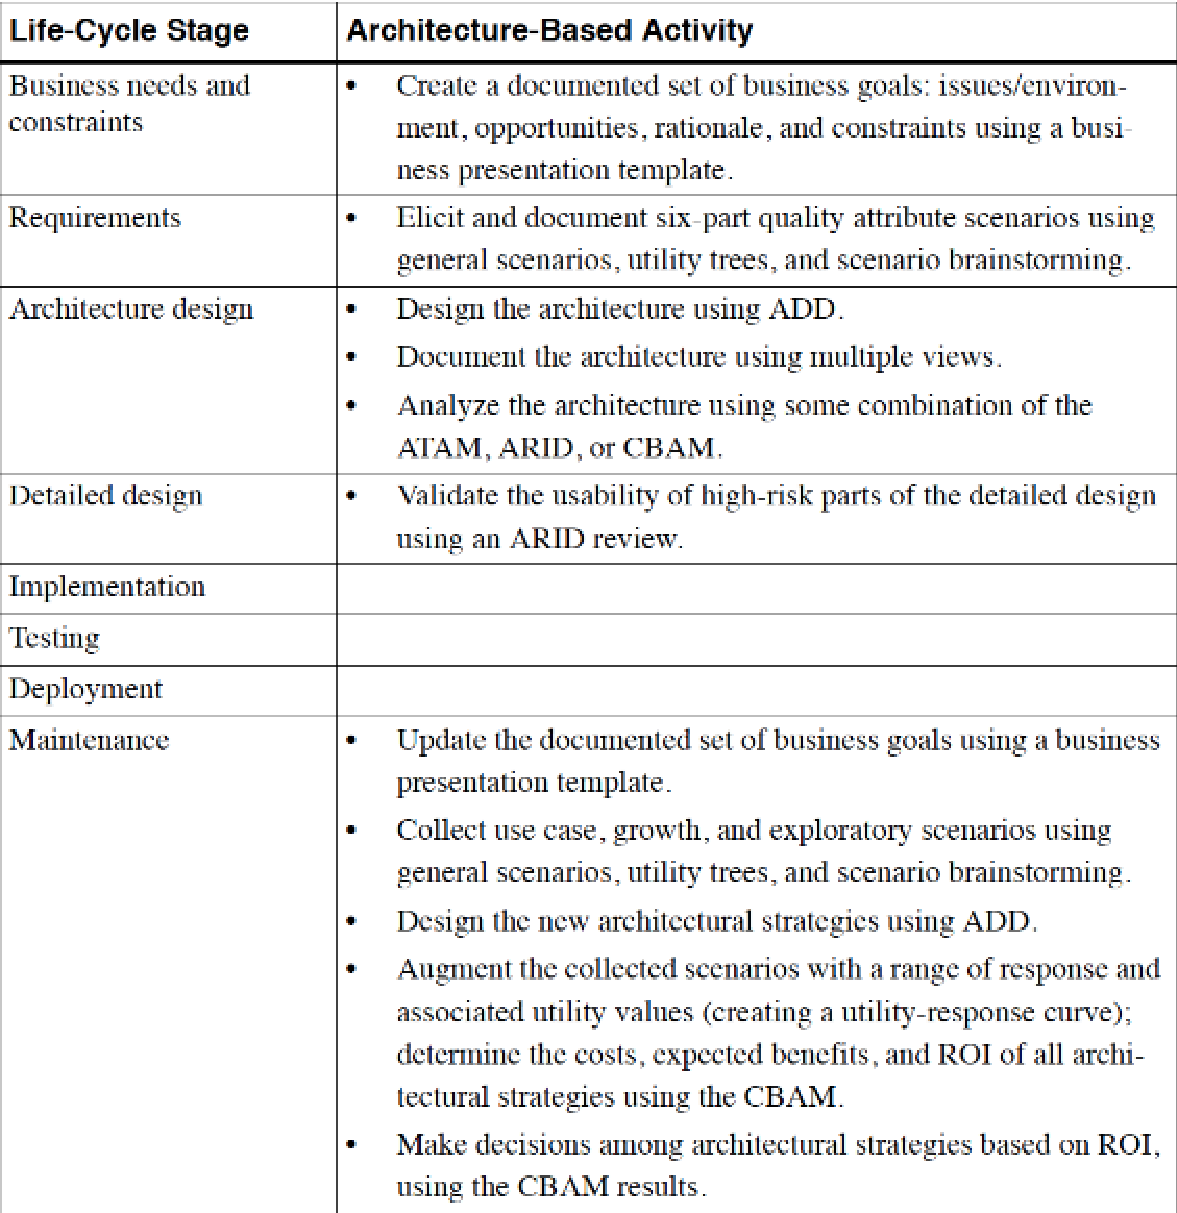
\includegraphics[scale=0.5]{images/LifecycleStages.pdf}
\end{center}
\end{figure}

The images on the next few pages show the typical stages of the software lifecycle and then typical examples of different software lifecycles.

\begin{figure}[H]
\begin{center} 
    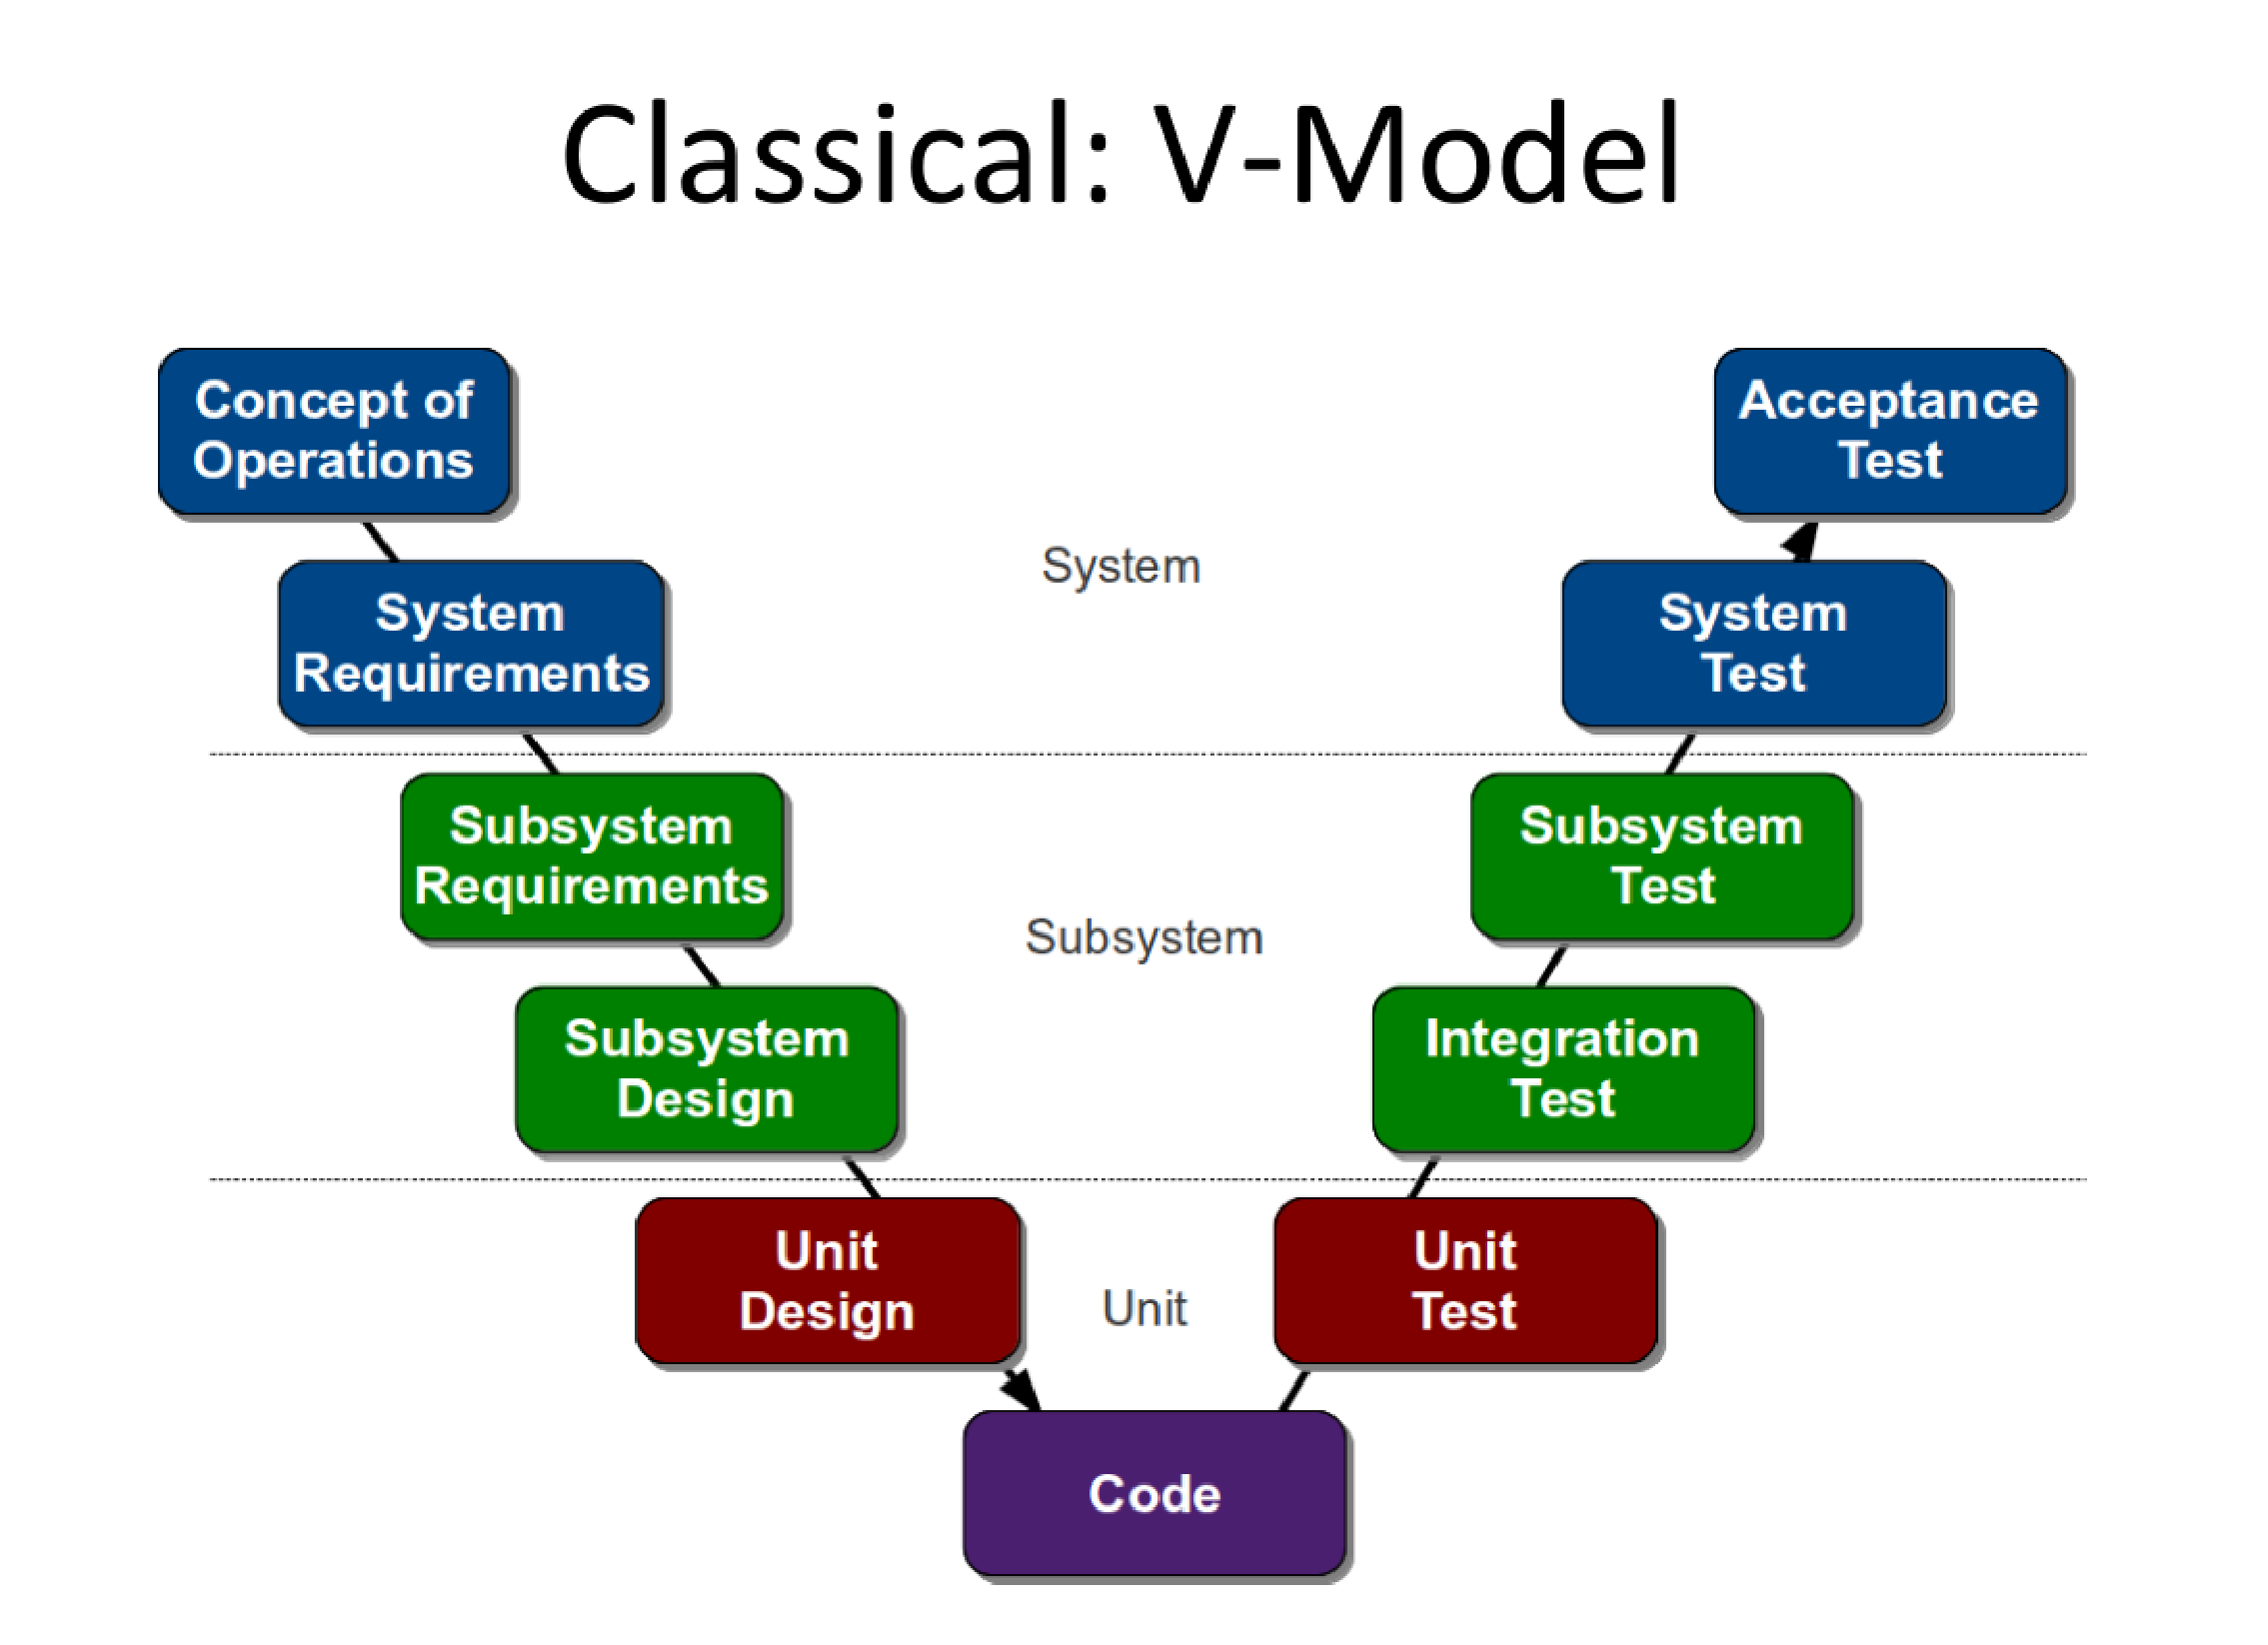
\includegraphics[scale=0.3]{images/VModel.pdf}
    \caption{A diagram showing the V model}
\end{center}
\end{figure}

\begin{figure}[H]
\begin{center} 
    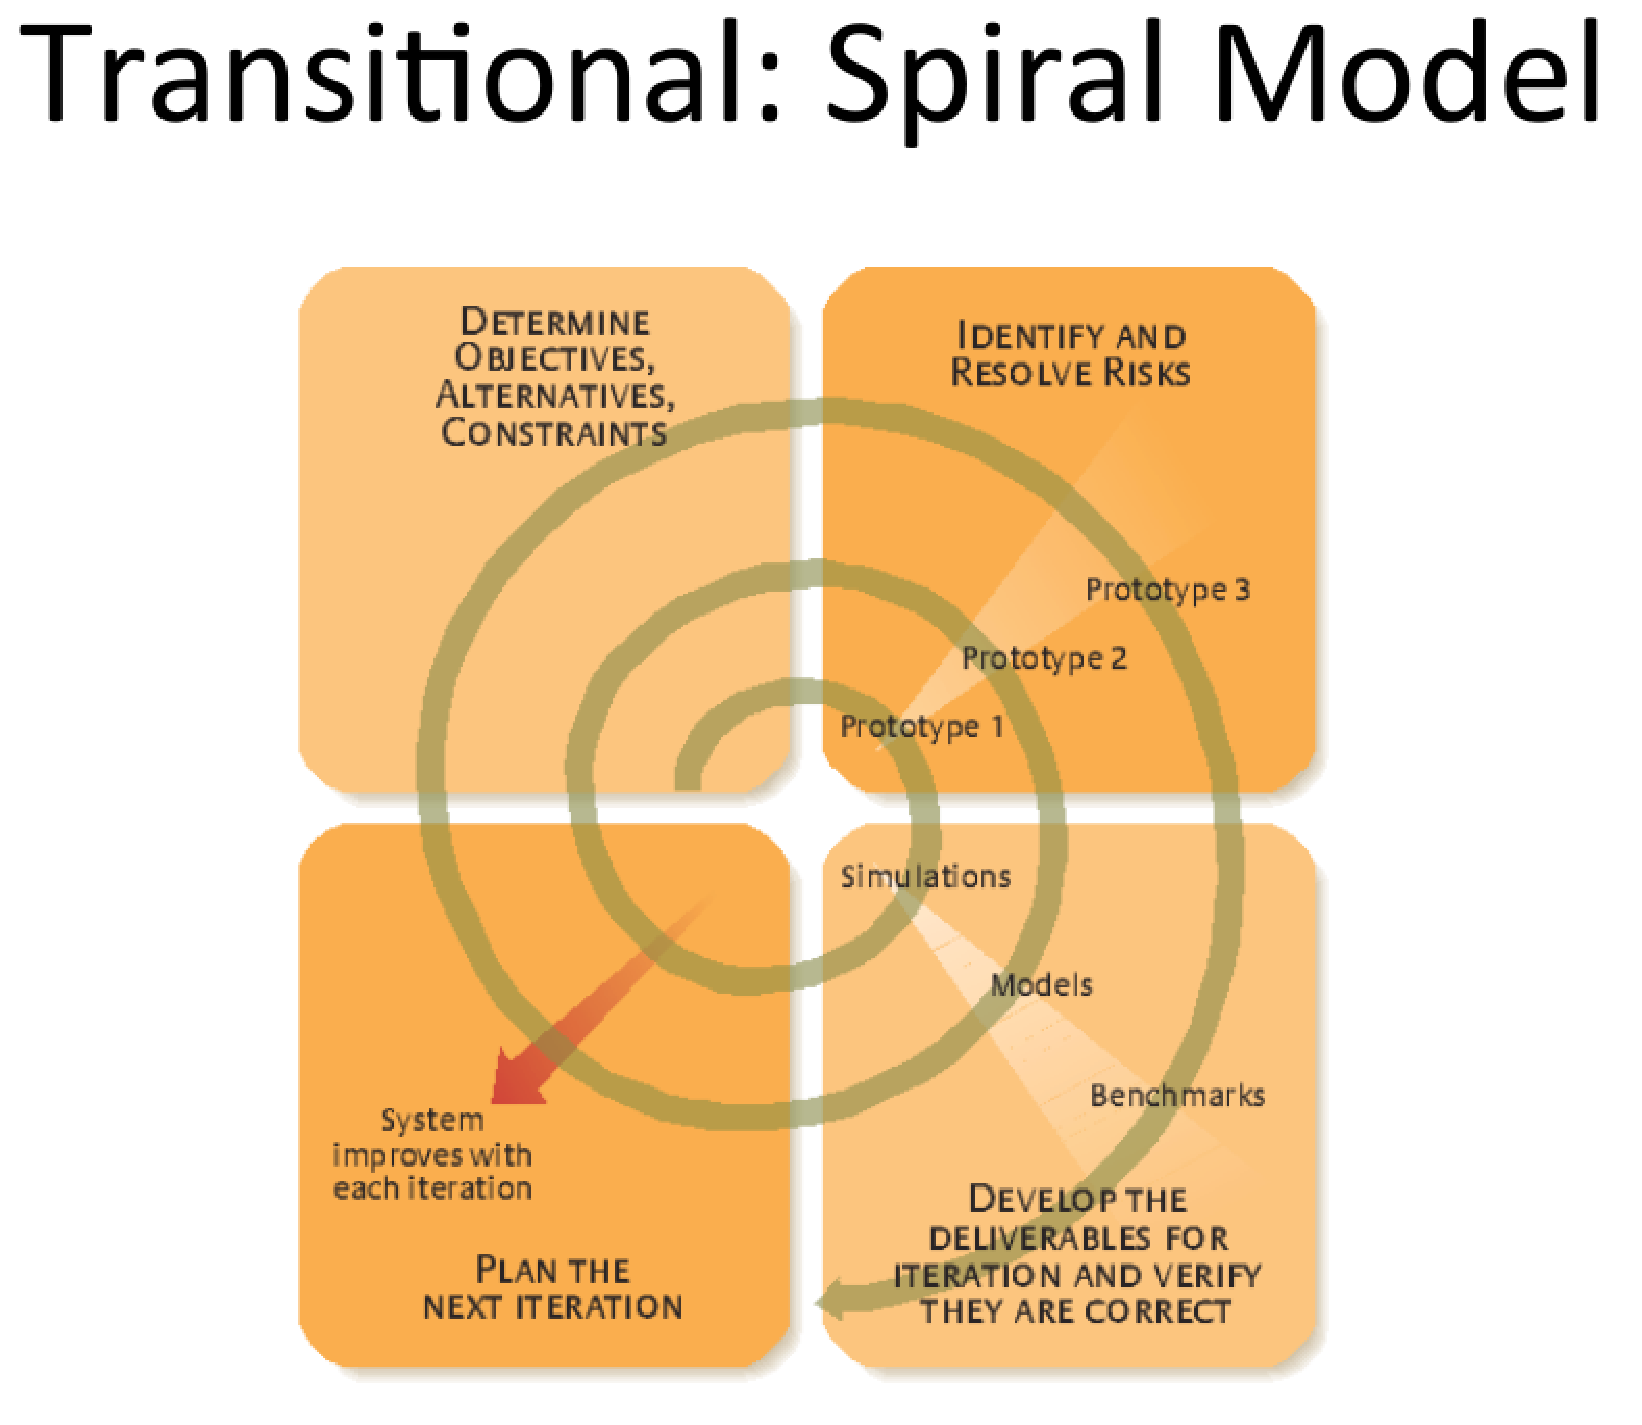
\includegraphics[scale=0.3]{images/Spiral.pdf}
    \caption{A diagram showing the spiral model}
\end{center}
\end{figure}

\begin{figure}[H]
\begin{center} 
    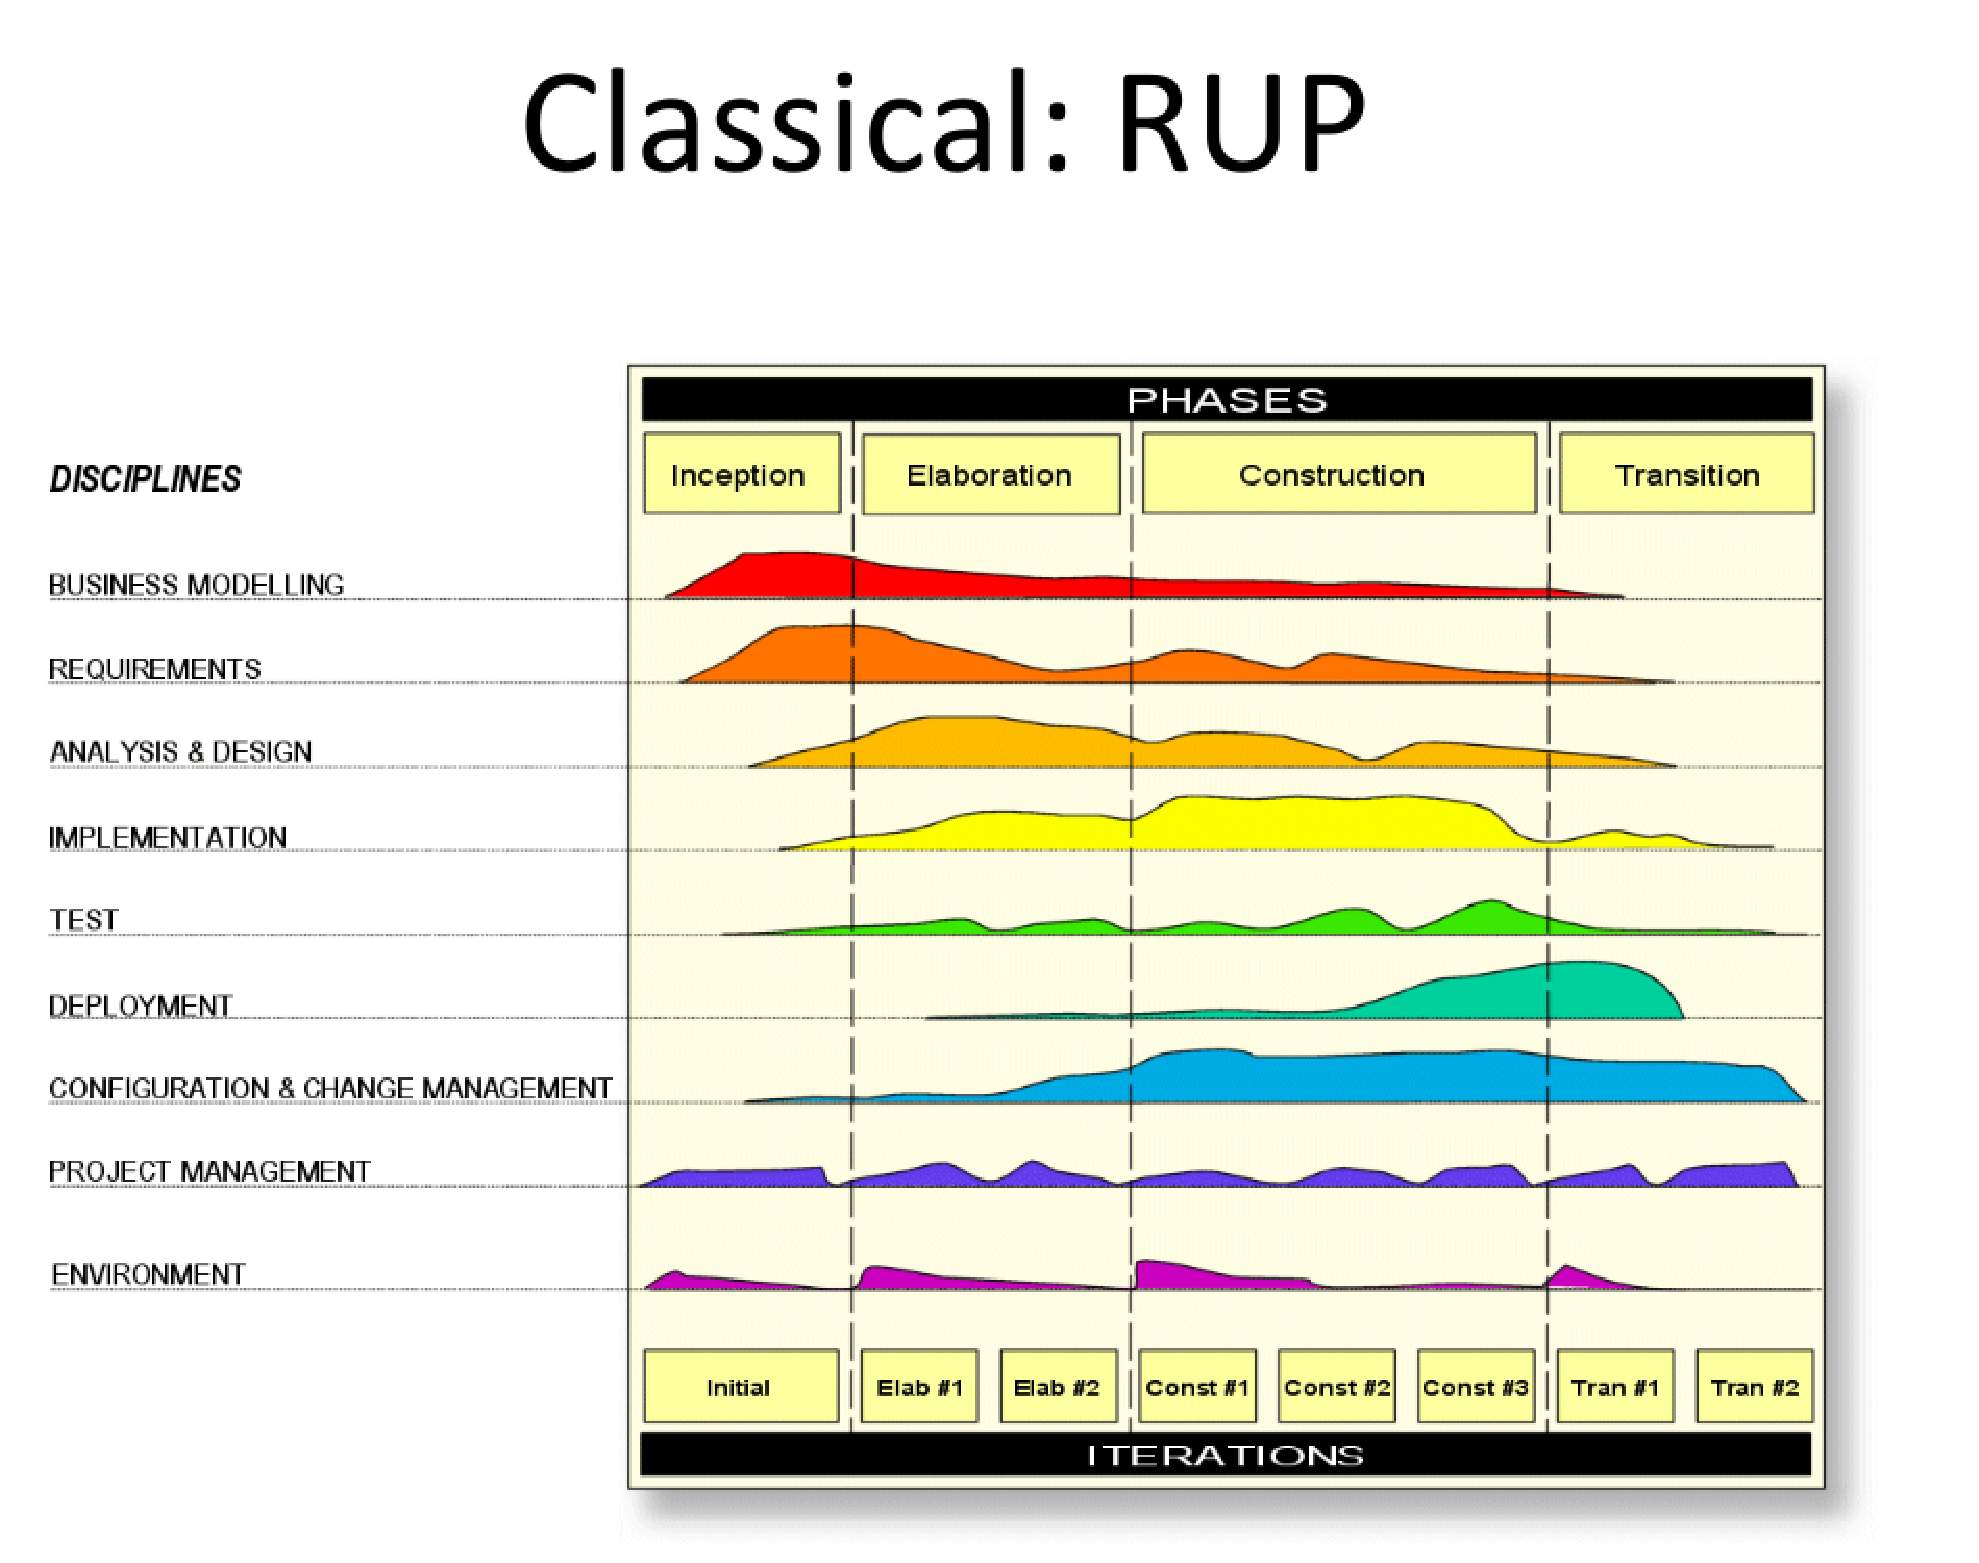
\includegraphics[scale=0.3]{images/RUP.pdf}
    \caption{A diagram of the RUP model}
\end{center}
\end{figure}

\textbf{Rational Unified Process(RUP) explained \newline} 
Rational Unified Process (RUP) establishes four phases of development, each of which is organized into a number of separate iterations that must satisfy defined criteria before the next phase is undertaken: in the inception phase, developers define the scope of the project and its business case; in the elaboration phase, developers analyze the project's needs in greater detail and define its architectural foundation; in the construction phase, developers create the application design and source code; and in the transition phase, developers deliver the system to users. 


\subsection{Agile Programming}
Agile Programming Practice:
\begin{itemize}
\item Test first programming
\item Refactoring
\item Continuous integration
\item Simple design
\item Pair programming
\item Common codebase
\item Coding standards
\item Open work area
\end{itemize}

Manifesto for Agile Software Development:
\begin{itemize}
\item Individuals and interactions over processes and tools.
\item Working software over comprehensive documentation.
\item Customer collaboration over contract negotiation.
\item Responding to change over following a plan.
\end{itemize}

The terms on the right are valued, but those on the left are valued more.

Scrum is an Agile framework for completing complex projects. Scrum originally was formalized for software development projects, but it works well for any complex, innovative scope of work. The possibilities are endless. The Scrum framework is deceptively simple:

\begin{itemize}
\item A product owner creates a prioritized wish list called a product backlog.
\item During sprint planning, the team pulls a small chunk from the top of that wish list, a sprint backlog, and decides how to implement those pieces.
\item The team has a certain amount of time — a sprint (usually two to four weeks) — to complete its work, but it meets each day to assess its progress (daily Scrum).
\item Along the way, the ScrumMaster keeps the team focused on its goal.
\item At the end of the sprint, the work should be potentially shippable: ready to hand to a customer, put on a store shelf, or show to a stakeholder.
\item The sprint ends with a sprint review and retrospective.
\item As the next sprint begins, the team chooses another chunk of the product backlog and begins working again
\end{itemize}

\subsection{Comparison of Agile versus Plan-Driven Approach}
The tables in the following images compare the agile to a plan-driven approach. 
\begin{figure}[H]
\begin{center} 
    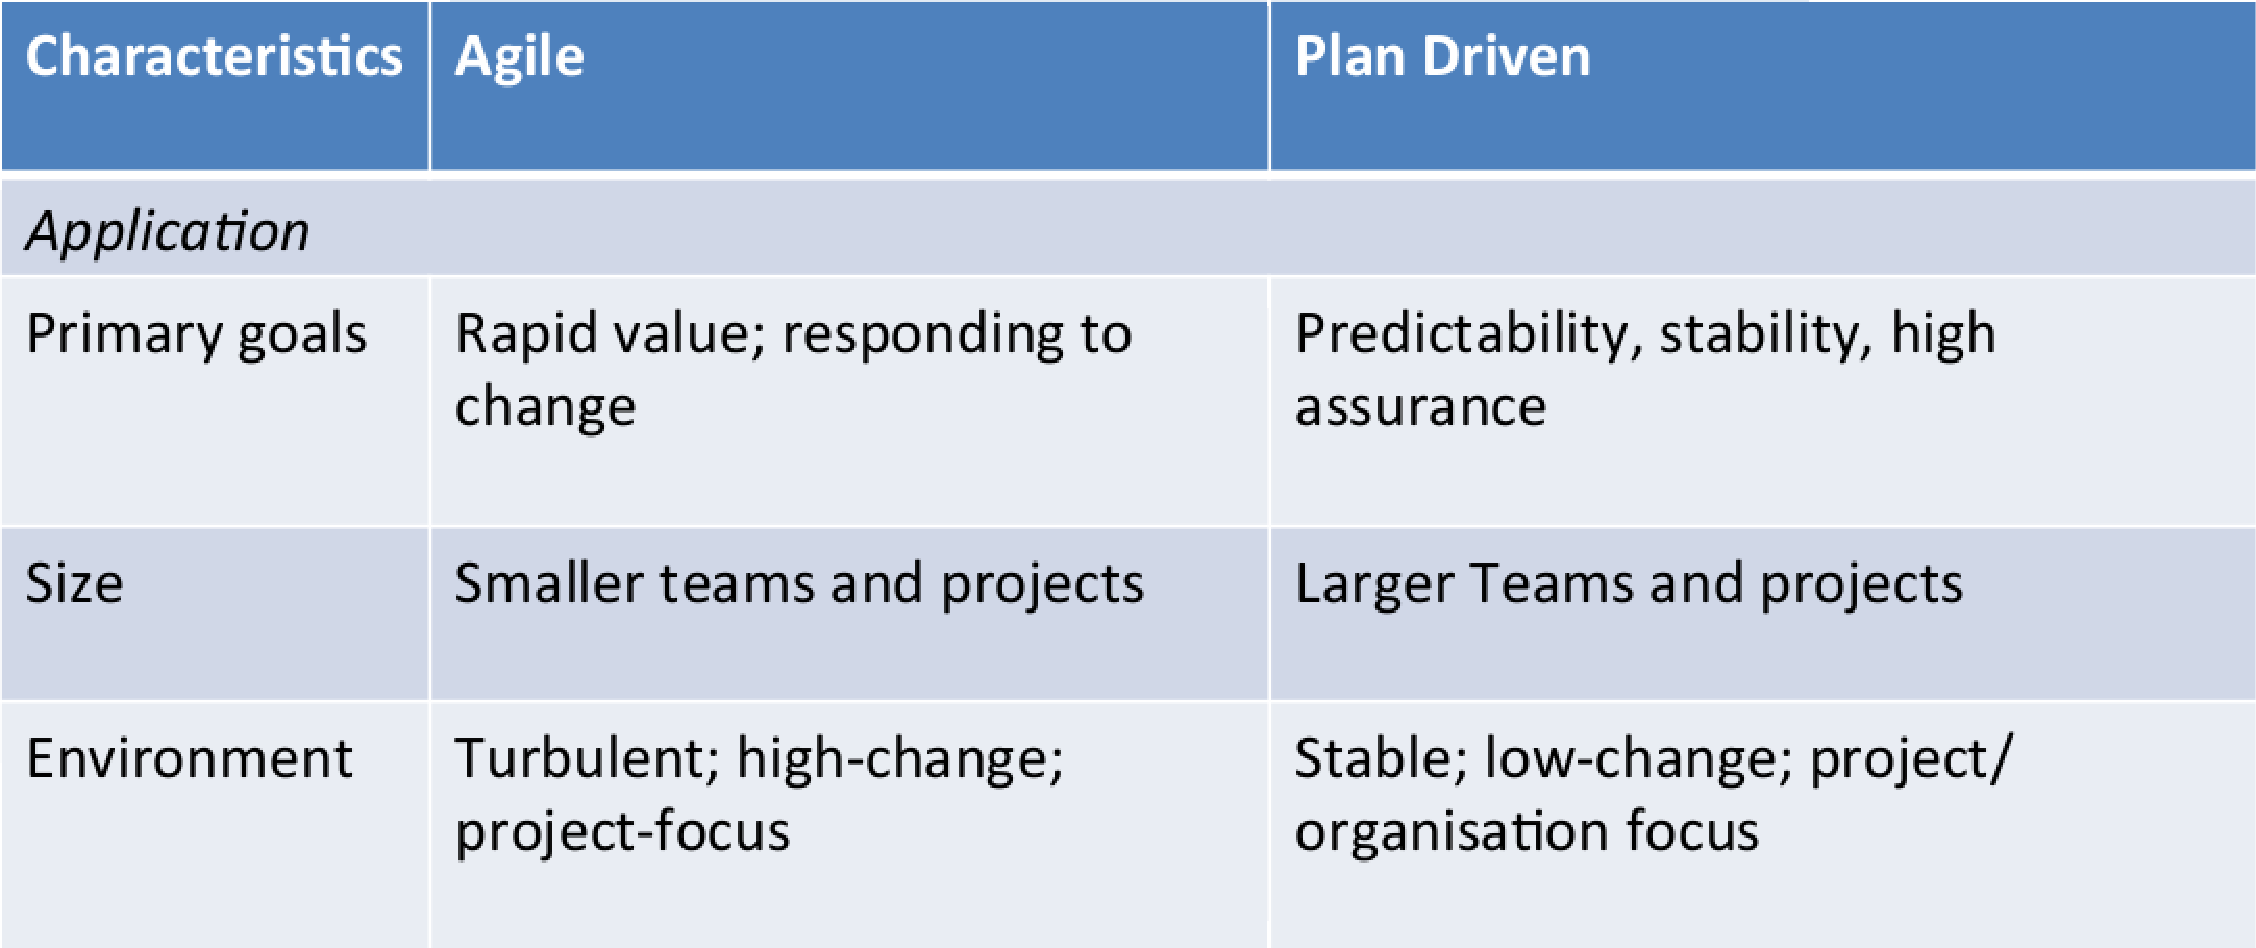
\includegraphics[scale=0.3]{images/AgileTable1.pdf}
\end{center}
\end{figure}

\begin{figure}[H]
\begin{center} 
    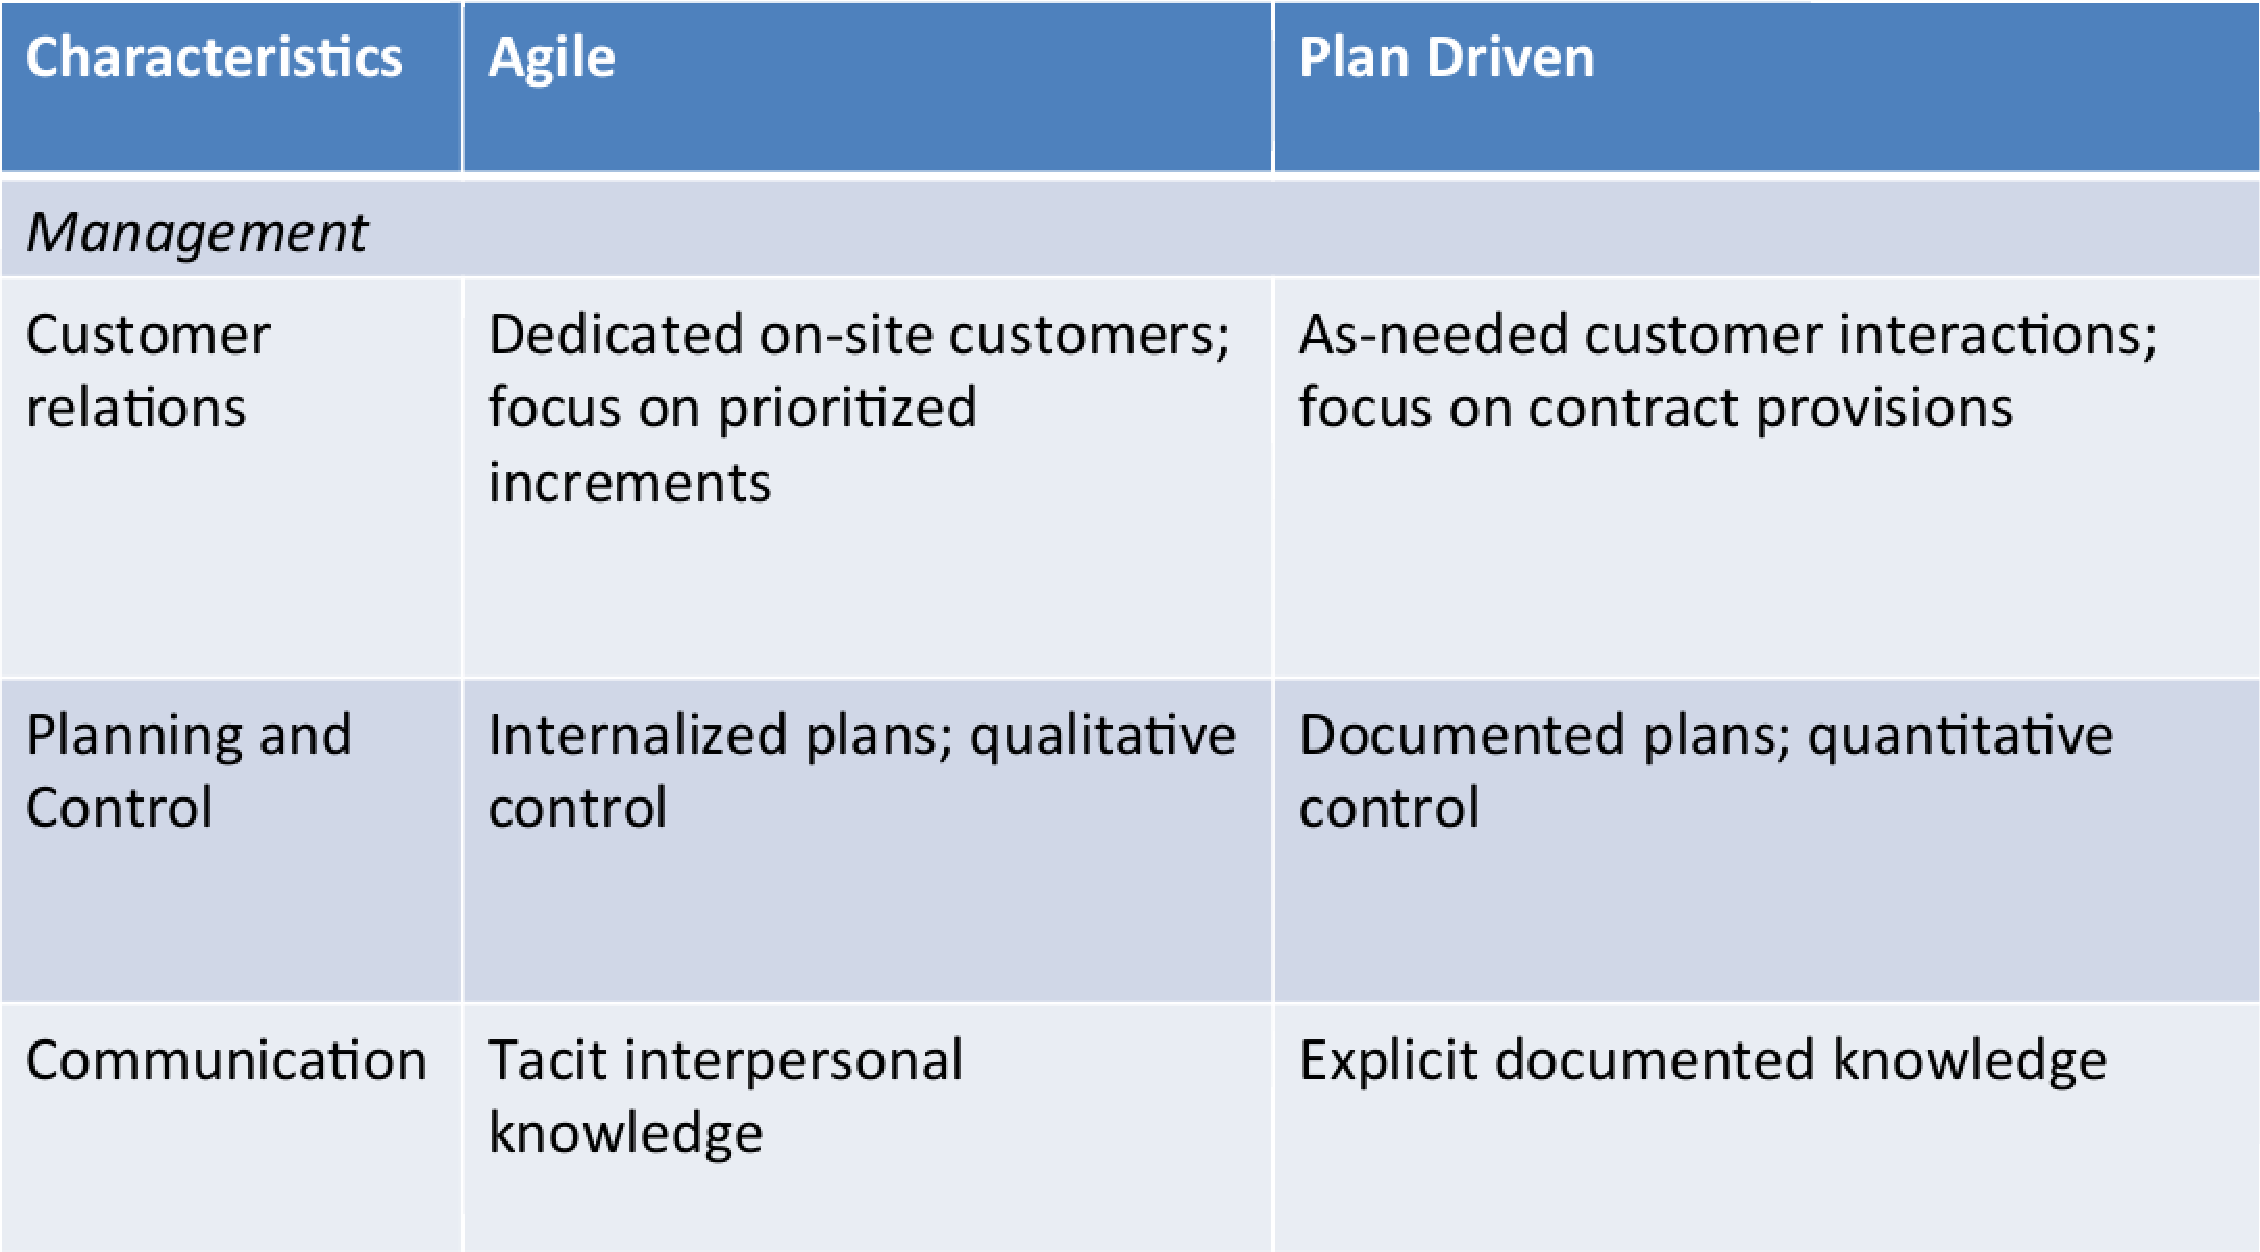
\includegraphics[scale=0.3]{images/AgileTable2.pdf}
\end{center}
\end{figure}

\begin{figure}[H]
\begin{center} 
    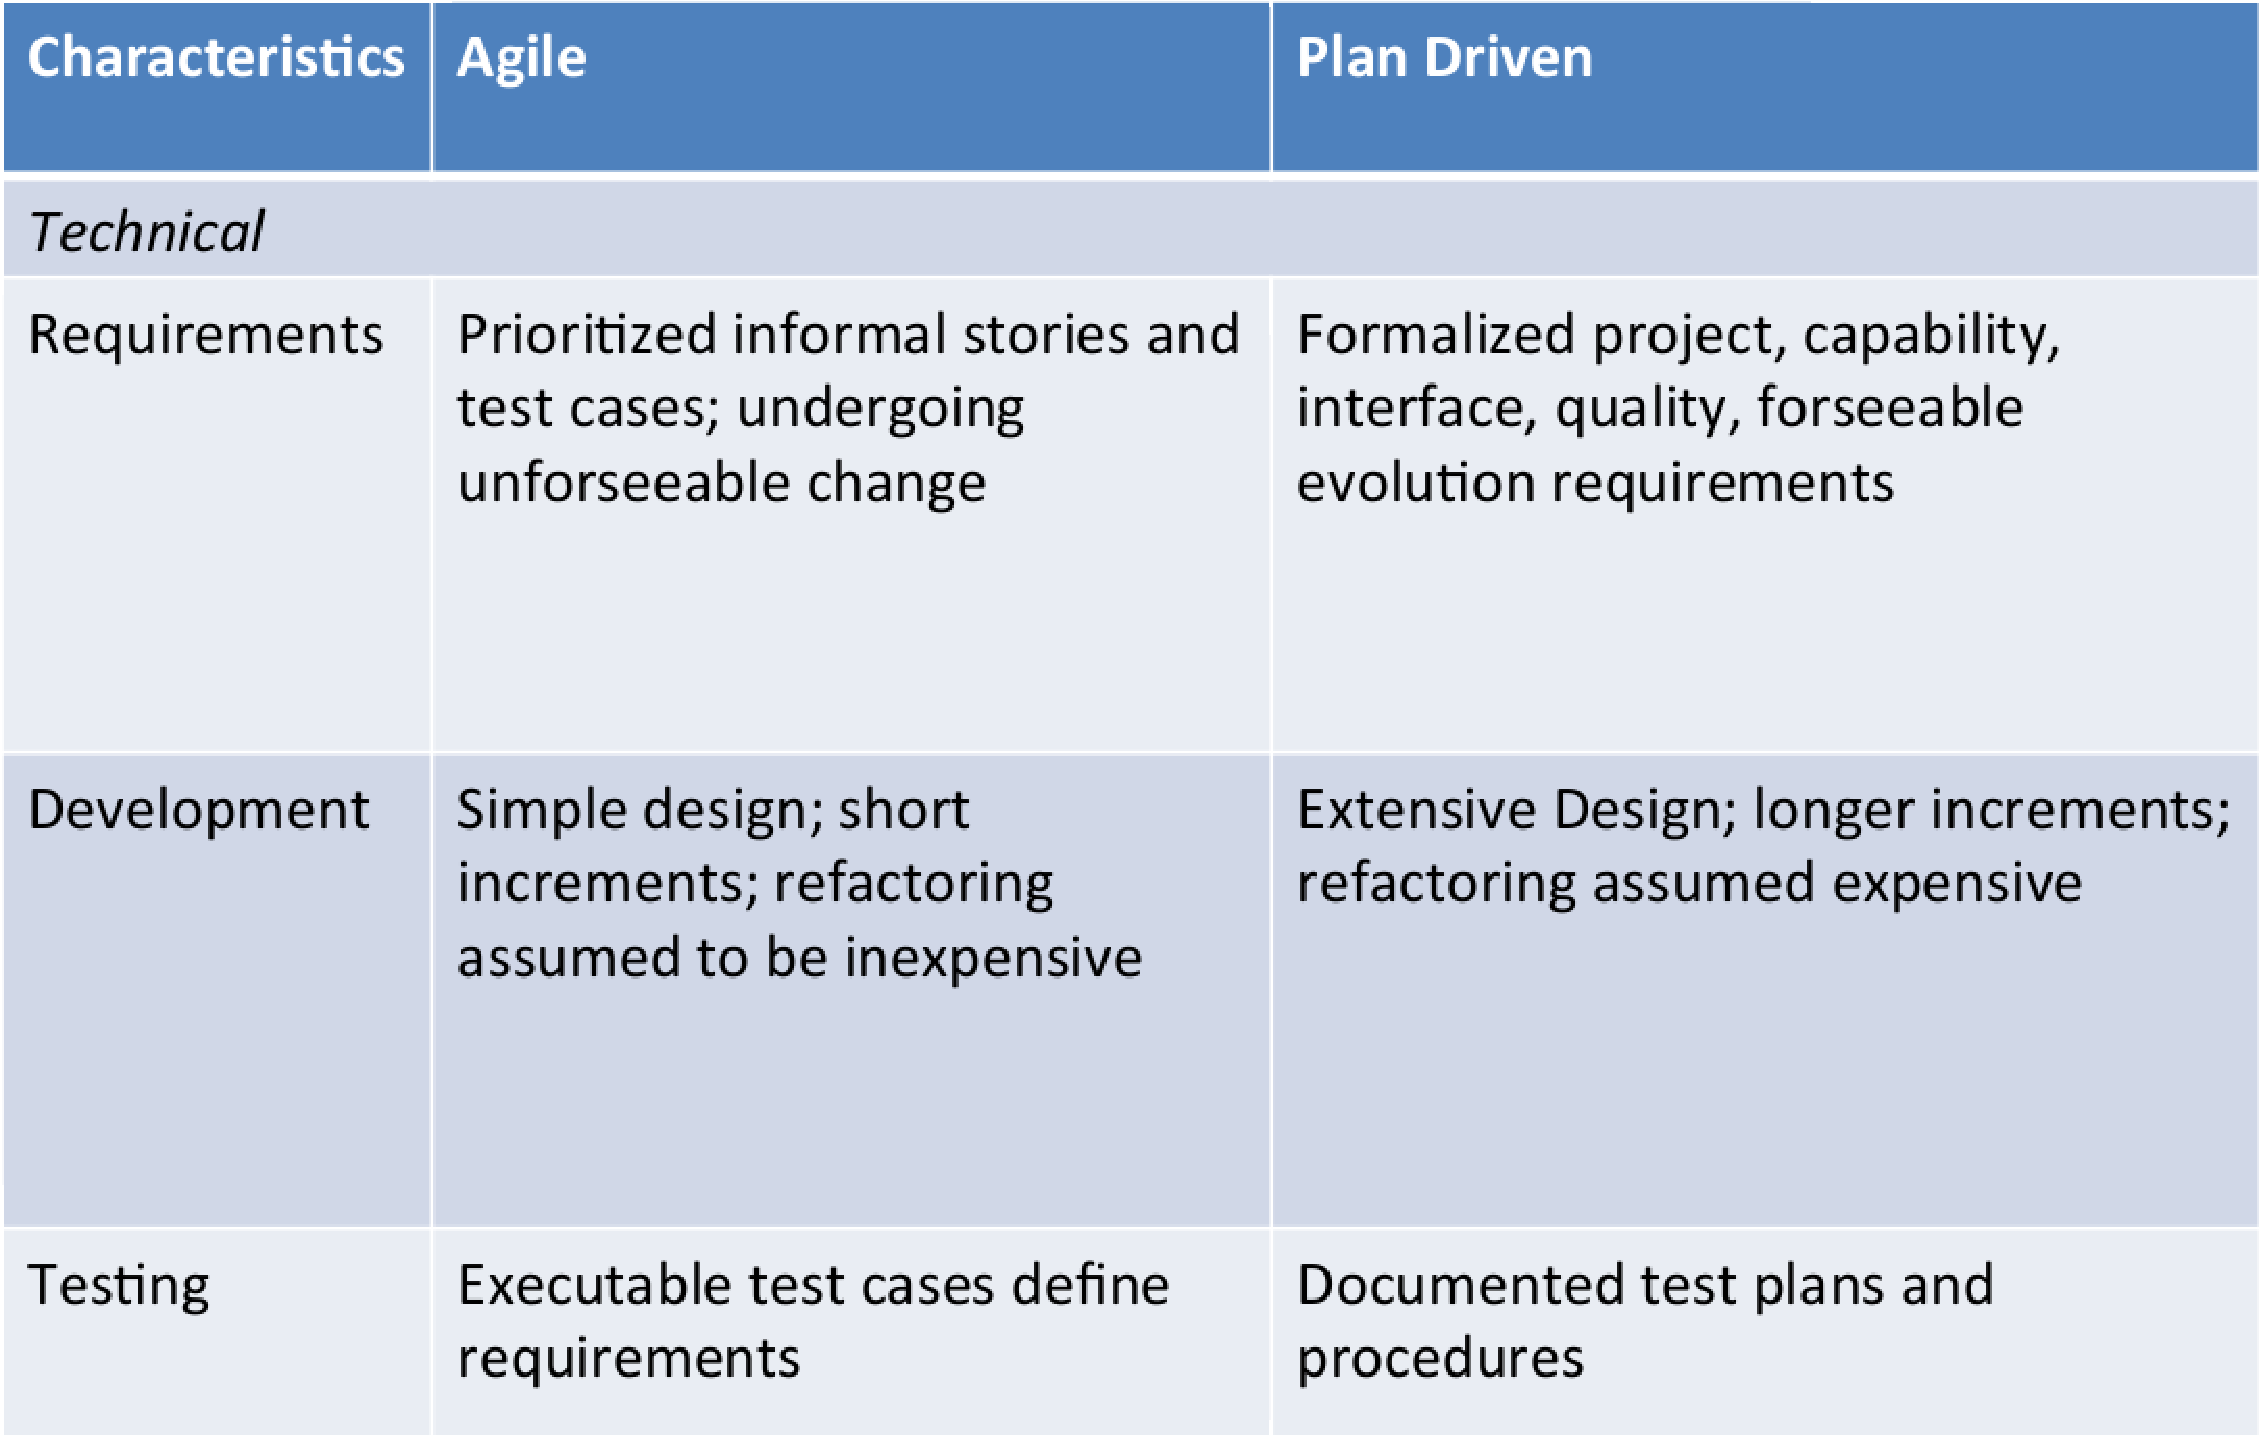
\includegraphics[scale=0.3]{images/AgileTable3.pdf}
\end{center}
\end{figure}

\begin{figure}[H]
\begin{center} 
    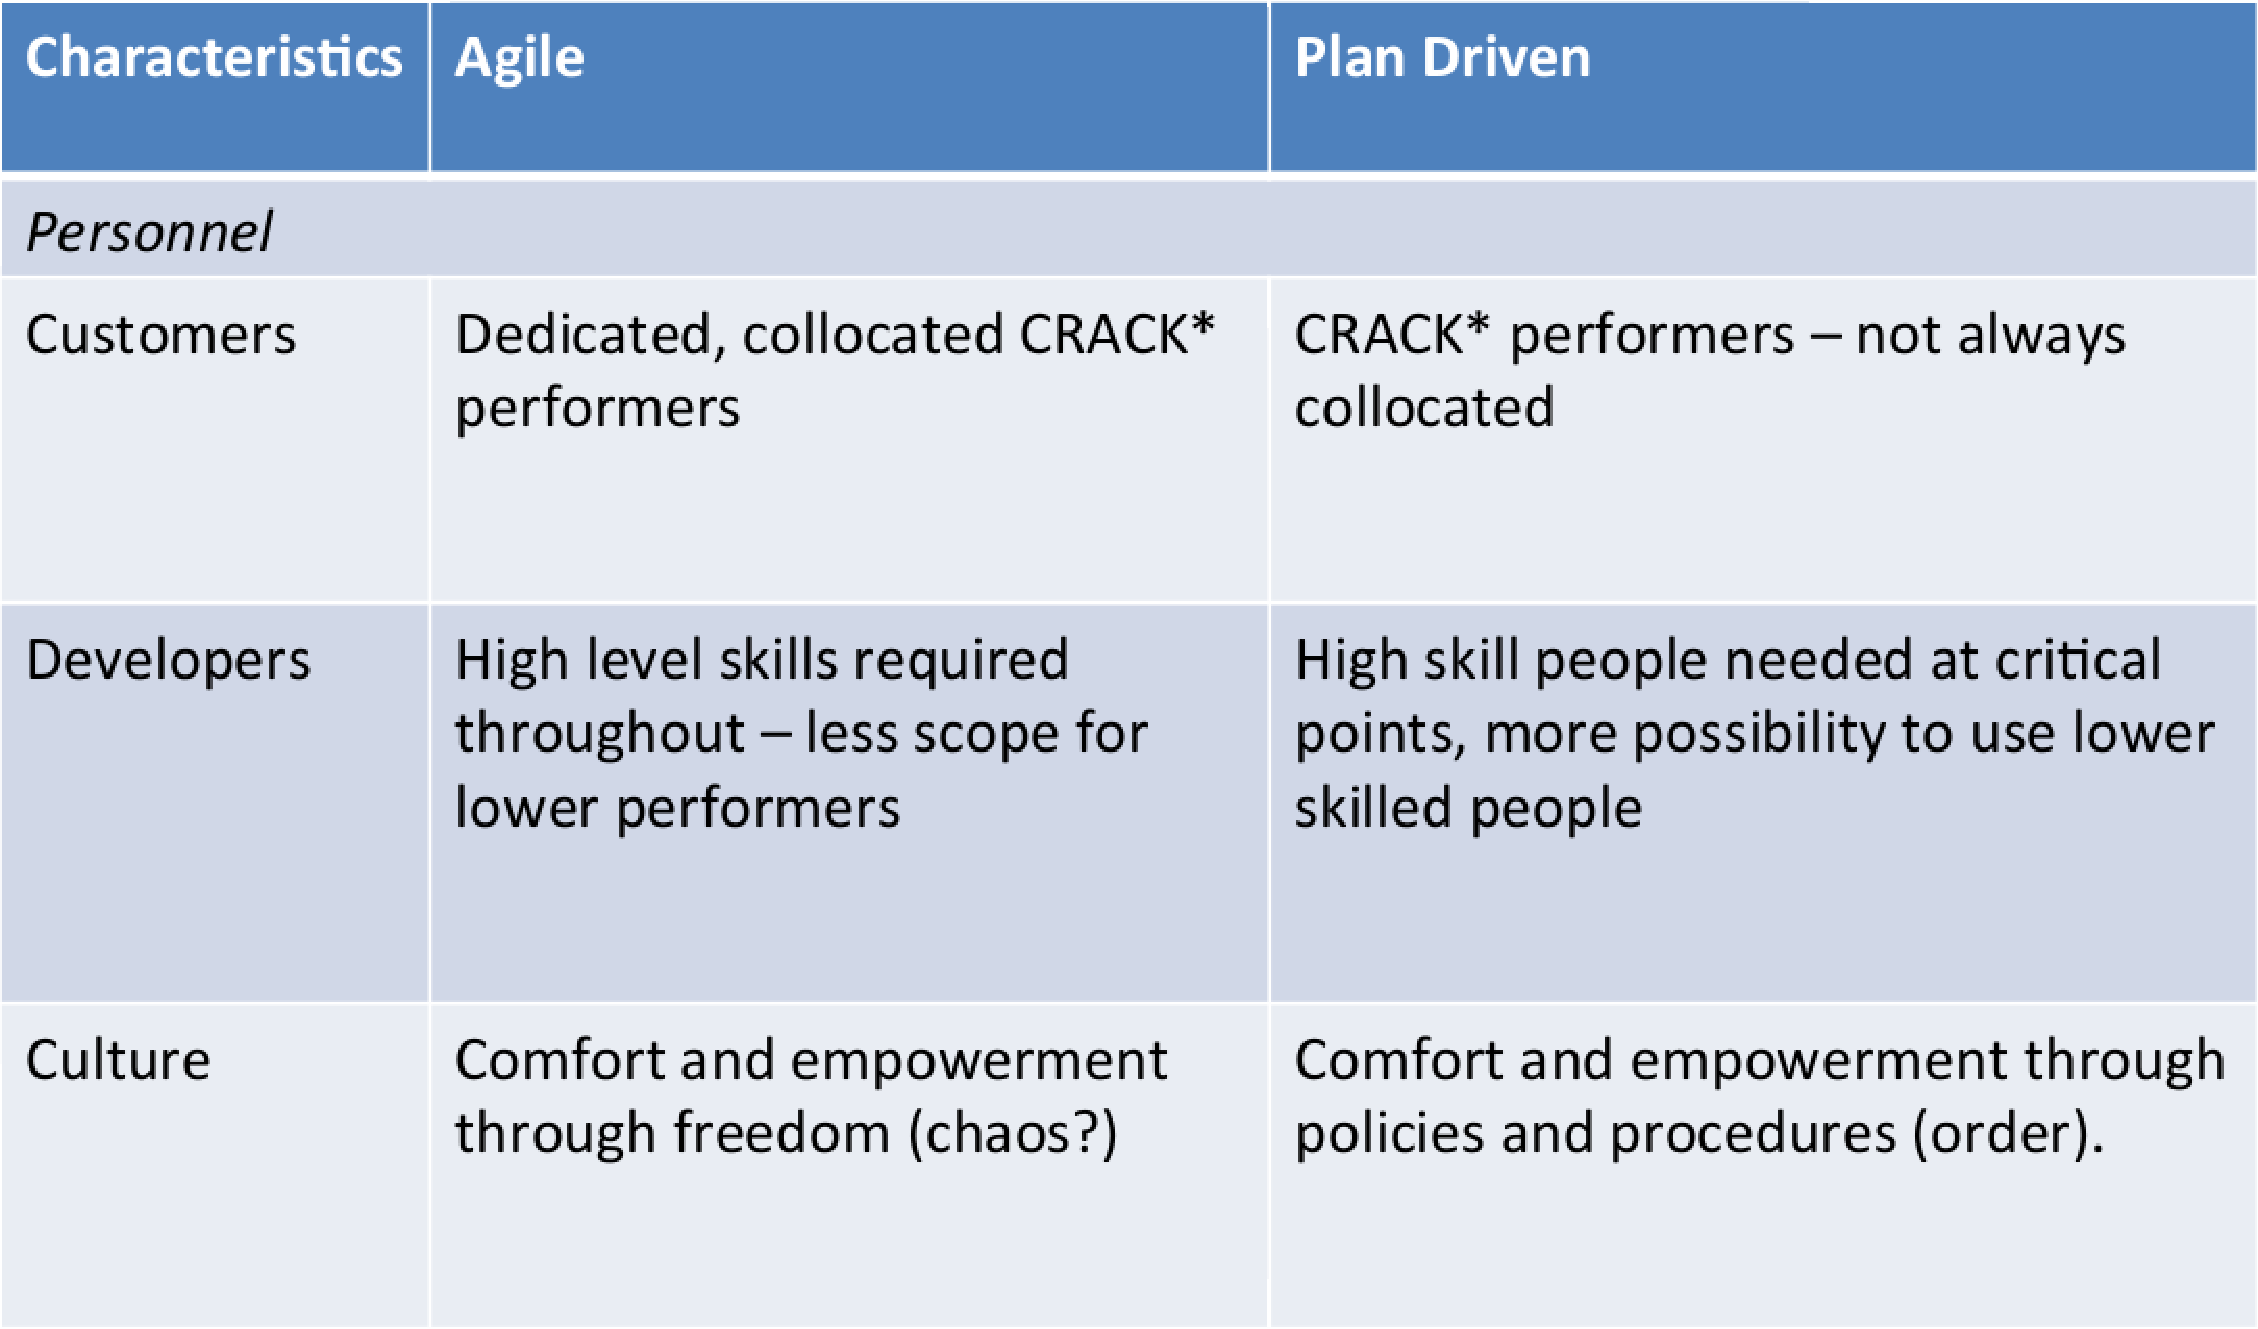
\includegraphics[scale=0.3]{images/AgileTable4.pdf}
\end{center}
\end{figure}

Key Points:
When developing software, work top-down and bottom-up at the same time – the balance of this depends on the size and complexity of the project.

General Rule:
As the size of the error/loss increases, the probability of the loss decreases. When the loss is small, the probability of it occurring is high. The relationship varies slightly depending on the project, but the general trend is as described above.

\begin{figure}[H]
\begin{center} 
    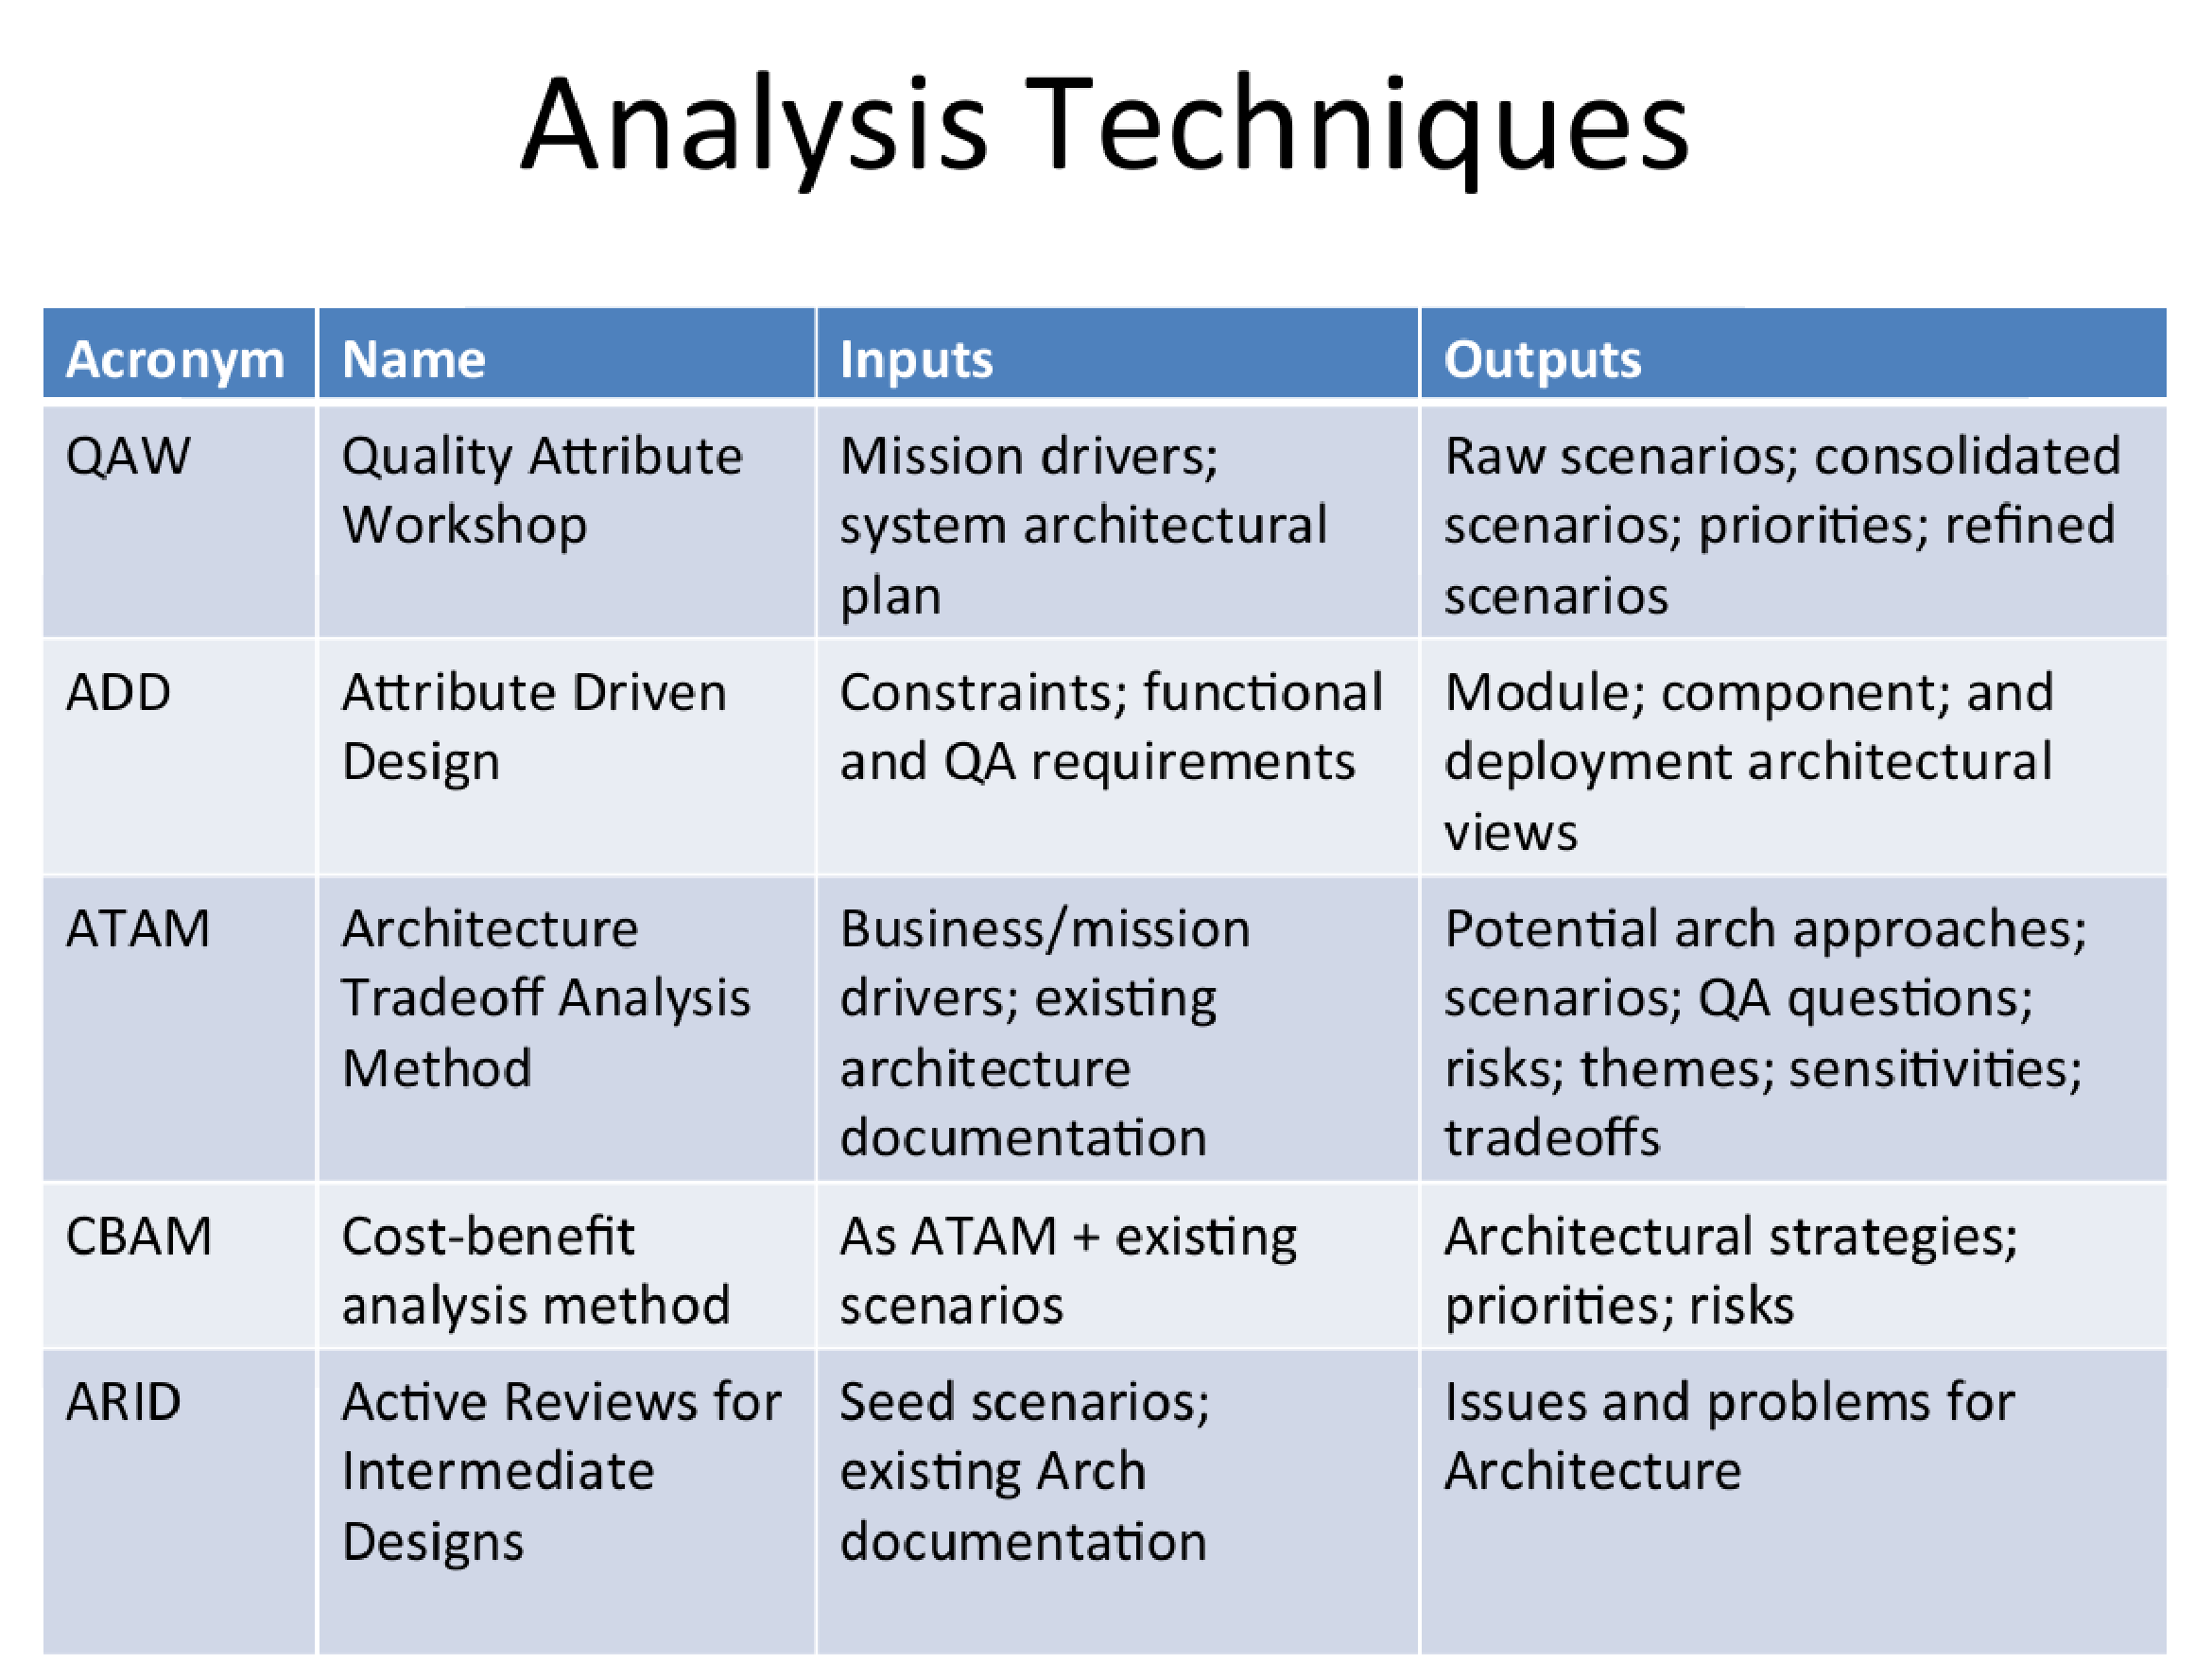
\includegraphics[scale=0.3]{images/Analysis1.pdf}
    \caption{Analysis Techniques}
\end{center}
\end{figure}

\begin{figure}[H]
\begin{center} 
    \includegraphics[scale=0.3]{images/Analysis2.pdf}
    \caption{Analysis Technique and Stage}
\end{center}
\end{figure}

\subsection{Summary}
\begin{itemize}
\item There are	many possible lifecycles and variants on	
these lifecycles.	
\item For any partcular	area of	actvity	we need to find the	
balance	between	agility	and	discipline.	
\item  Risk	links	discipline	and	agility	
\item QAs, scenarios and tactics help link architecture to	
more agile practice.	
\item Architectural	analysis techniques	provide	useful	
information for lifecycle activities, however they are	
arranged in	a process.	
\item Processes	like the Spiral	Model or ICM provide	
processes that are	sensitive to project risk.
\end{itemize}

\newpage
\section{Dev-Ops}
This is the process of seeing development and operations as a unified entity. It oversees the whole process and all stages of developing software. It is the set of practices intended to reduce the time between communicating a change to a system and the change being placed into normal operation while ensuring necessary quality. 

The Whole Application Lifecycle:
1)  Define - ideation
2)  Develop - idea to working software
3)  Operate - working software in production, value realization
4)  Measure - actionable learning

\subsection{OSLC}
OSLC standards simplify lifecycle integration, which leads to cost savings and increased flexibility.
It is the foundational technology for all integration, and is the natural choice for standardizing loosely-coupled integrations in new domains. 

\begin{figure}[h]
\begin{center} 
    \includegraphics[scale=0.8,width = 15cm, height = 12cm]{images/OSLC.pdf}
    \caption{Summary of OSLC}
\end{center}
\end{figure}

\subsection{Critical Points in the Lifecycle of Software}
\begin{itemize}
\item  Make the decision to commit the code to be introduced into the system.
\item  Transition from something being just under consideration to actually being a key part of the system.
\item  Do we have enough confidence to be able to make such a transition?
\item  We want to ensure each of these transitions are as reliable as possible. 
\end{itemize}

\subsection{Microservices Architectural Pattern}
Puts each element of functionality (small, single purpose) into a separate service and scales by distributing these services across servers, replicating as needed. They are loosely coupled and asynchronous.

\subsection{How to make development easier, faster, and better}
\begin{itemize}
\item One step environment creation – need a common environment build process
\item Code, environment, and configuration all in one place
\item Automation is essential
\item Feedback loops – understanding and responding to the needs of all customers (both internal and external) – automate these feedback loops
\end{itemize}
Having such a consistent process and effective feedback results in agility – then can experiment, fail, but learn and recover quickly.

It is important to see your mistakes before you actually start producing the software on a wide scale: 
\begin{itemize}
\item Be consistent in the code, environments, and configuration
\item Try to catch misconfiguration and inconsistencies early
\item Testing every feature as you are building the system
\item Try to limit technical debt 
\end{itemize}
Technical Debt - concept in programming that reflects the extra development work that arises when code that is easy to implement in the short run is used instead of applying the best overall solution

\newpage
\section{Product Line Architecture}
Software often comes in families. Thus, it makes sense to try to share components. Many real-world products are produced in a product line – such as cras, for example.

A software product line is a collection of software-intensive systems that share a common, managed set of features that are developed from a set of core assets in a prescribed way. 

Think of different, successive versions of the same product released by a company – they are all based on the same baseline architecture. When the number of products in it increase beyond a certain number, it starts to become profitable for the company using this technique.

\subsection{Key Properties}
Key properties of this product line architecture:
\begin{itemize}
\item usually are directed by the business goals in the application domain
\item all products share a software product line architecture
\item new products are all structured by this product line architecture and are built from services and components
\item product lines spread costs over several products
\item Architecture must be flexible enough to support variation in the products
\item Software components – general enough to support variability
\item All other components of the software must be general enough to deal with variation
\item People need to be skilled in architecture and product lines
\end{itemize}

\subsection{Benefits to organization}
There are several benefits to the organization:
\begin{itemize}
\item much better productivity
\item quicker delivery time to the market – so maintain market presence and sustain growth
\item enable mass customization
\item improve product quality
\item better predictability of cost, schedule, and quality
\end{itemize}

\subsection{Main Terms}
\textbf{Core Asset Development:} improving the base components in terms of qualities, products they support, and architecture

\textbf{Product Development:} identifying and building products to meet market need inside the product line

\textbf{Management:} monitoring and improving the processes, tools, and practices

\subsection{Different Techniques in Introducing Product Lines}
\begin{itemize}
\item Proactive – up front investment to develop the core assets
\item Reactive – start with one or two products and use them to generate core assets – so see how well they do and then “react”
\item Incremental – develop core assets as the business need evolves
\end{itemize}
The general process involves considering the business strategy, consequences for products, consequences for processes and methods, and consequences for tools and the organization.

\subsection{Pros of Using a Product Line:}
\begin{itemize}
\item Increased competitiveness on the market because of reduced hardware resource consumption and reduced time to market for new features
\item Development efficiency – reuse, easy configuration of software products, increased planning accuracy
\item Quality  - interface integrity, reuse of core assets
\item Customer needs – differentiation by individual software solutions, clear feature-cost mapping
\end{itemize}

\subsection{Architectural Features of Product Lines:}
\begin{itemize}
\item Control of resource consumption, such as memory
\item Good interface management
\item Layers provide the opportunity to share applications without knowing the details of some components
\item Software is reusable so that component redesign is easy and quick
\item Standardization is important
\item Important to standardize and develop tools that ease interchange between the company and it clients (toolchains)
\end{itemize}

\subsection{Phased Introduction}
This is how a company would start applying a software product line (called phased introduction) :
\begin{itemize}
\item Investigate and customize product line engineering
\item Design and apply adequate processes and methods
\item Roll out and institutionalize the standard development process
\end{itemize}

\newpage
\section{Analysis}
Why we Evaluate:
\begin{itemize}
\item To inform decision making
\item To allow progression to later stages in to process (think sprial/ incremental development methodologies)
\end{itemize}

There are three types of Evaluation:
\begin{itemize}
\item Evaluation By Designer
\item Peer Evaluation
\item External Evaluation
\end{itemize}

\subsection{Evaluation By Designer}
The consequences of the decision regulate how much effort to put into the process $\rightarrow$ more importance means more effort in evaluation. Try to use iterative approaches that get deeper in order to eliminate unpromising alternatives early. \textit{(Don't strive for perfection, good enough for the context is usually good enough)}

\subsection{Peer Evaluation}
Fix the \textit{Quality Attributes} to consider as part of the review $\rightarrow$  maybe determined by the process or the business case. The \textbf{architect} presents the architecture to the reviewers (the questions are for information). The review is driven by the relevant scenarios the architect talks the review team through a scenario demonstrating the architecture meets the requirements captured in a scenarios.

\subsection{External Evaluation}
Means to bring in additional expertise. Maybe represent some stakeholder interests. It is a more \textbf{expensive} evaluation method and difficult to organise so this will often correspond to some major hurdle in the process.


These may include, but are not limited to \textbf{(contextual factors)}:
\begin{itemize}
\item What artefacts are available?
\item Who sees the results of the review?
\item Who preforms the evaluation?
\item Which stakeholders will participate?
\item How does the evaluation relate to business goals of the system?
\end{itemize}


\subsection{Additional Info}

When we evaluate shit we must consider \textbf{Contextual Factors} as well.

In summary, the	larger and	more complex the system the more likely you are to have done explicit architectural design and any design should be evaluated.
 







\end{document}
